\documentclass[11pt,a4paper,twoside,openright]{report}

\usepackage[nottoc,notlot,notlof]{tocbibind}
\usepackage[pdftex]{graphicx}
\usepackage{tabularx}
\usepackage{multirow}
\usepackage{subcaption}
\usepackage{afterpage}
\usepackage{amsmath,amssymb,amsthm}
\usepackage{rotating}
\usepackage{fancyhdr}
\usepackage{tikz}
\usepackage{rotating}
\usepackage{float}
\usepackage[pdfusetitle, colorlinks, linkcolor=black, citecolor=black, urlcolor=black]{hyperref}
\usepackage{algorithm}
\usepackage{algpseudocode}
\usepackage{pgf,pgfplots}
\pgfplotsset{compat=1.15}
\usepackage{mathrsfs}
\usepackage{colortbl}
\usepackage{hhline}


\usetikzlibrary{arrows}
\usepackage{mathtools}
\usepackage{rotating}
%per fare elenchi puntati poco distanziati
\usepackage{enumitem} 
\usepackage[round]{natbib}
\usepackage[T1]{fontenc}
\usepackage{bm}
\usepackage{dsfont}



\usepackage{amssymb}% http://ctan.org/pkg/amssymb
\usepackage{pifont}% http://ctan.org/pkg/pifont
\newcommand{\cmark}{\ding{51}}%
\newcommand{\xmark}{\ding{55}}%








\setlength{\oddsidemargin} {2. cm}
\setlength{\evensidemargin} {2. cm}
\addtolength{\oddsidemargin} {-0.4 cm}
\addtolength{\evensidemargin} {-0.4 cm}
\linespread{1.1}

\usepackage[utf8]{inputenc}
\renewcommand{\captionfont}{\normalfont \itshape \small}


\pagestyle{empty}

\floatname{algorithm}{Algorithm}
\newcommand{\algorithmname}{Algorithm}

\newtheorem{theorem}{Theorem}
\newtheorem{corollary}{Corollary}[theorem]
\newtheorem{lemma}[theorem]{Lemma}
\newtheorem{definition}{Definition}
\newtheorem{example}{Example}
\newtheorem{problem}{Problem}
\newtheorem{prop}{Proposition}
\newtheorem{property}{Property}
\newtheorem{obs}{Observation}

\DeclareMathOperator*{\argmin}{arg\,min}
\DeclareMathOperator*{\argmax}{arg\,max}
\DeclareMathOperator*{\I}{\mathcal{I}}
\DeclareMathOperator*{\pl}{\mathcal{P}}
\DeclareMathOperator*{\T}{\mathcal{T}}
\DeclareMathOperator*{\F}{\mathcal{F}}
\DeclareMathOperator*{\B}{\mathcal{B}}
\DeclareMathOperator*{\A}{\mathcal{A}}
\DeclareMathOperator*{\ag}{\textbf{a}}
\DeclareMathOperator*{\pg}{\textbf{p}}


\newcommand{\Tmax}{T_{\textnormal{max}}} 
\newcommand{\Tmin}{T_{\textnormal{min}}} 
\newcommand{\Rmax}{R_{\textnormal{max}}} 
\newcommand{\Rmin}{R_{\textnormal{min}}} 

\DeclarePairedDelimiter{\ceil}{\lceil}{\rceil}
%\DeclareMathOperator*{\A}{\mathcal{A}}
%\DeclareMathOperator*{\argmax}{argmax}
\definecolor{cerise}{rgb}{0.87, 0.19, 0.39}



\renewcommand\Pr{\mathbf{P}\PrObject} % \Pr è già definito e lo vogliamo modificare
\DeclarePairedDelimiter{\PrObject}{(}{)}



\begin{document}

\thispagestyle{empty}
%\begin{titlepage}
\vspace*{-1.5cm} \bfseries{
\begin{center}
  \large
  POLITECNICO DI MILANO\\
  \normalsize
  Corso di Laurea Magistrale in Ingegneria 
  Informatica\\
  Dipartimento di Elettronica, Informazione e Bioingegneria\\
  \begin{figure}[htbp]
    \begin{center}
      
\includegraphics[width=3.5cm]{./images/logopm}
%	
\psfig{file=./pictures/logopm.png,width=3.5cm}
    \end{center}
  \end{figure}
  \vspace*{0.3cm} \LARGE



  \textbf{Multi-Armed Bandit with Persistent Reward}


  \vspace*{.75truecm} \large

\end{center}
\vspace*{3.0cm} \large
\begin{flushleft}


  Relatore: Prof. Francesco Trovò  \\
  Correlatore: Giulia Romano\\

\end{flushleft}
\vspace*{1.0cm}
\begin{flushright}


  Tesi di Laurea di:\\ Andrea Agostini\\ Matricola 900404 \\


\end{flushright}
\vspace*{0.5cm}
\begin{center}



  Anno Accademico 2019-2020
\end{center} \clearpage
}

\pagestyle{empty} \normalfont \cleardoublepage
%\include{contents/primapagina}
\cleardoublepage \pagenumbering{Roman} \pagestyle{plain}
%\include{contents/ringraziamenti}
%\vspace*{.75truecm} \cleardoublepage
\chapter*{\textbf{Sommario}}\vspace{-0.5cm}
In questa tesi studiamo
\addcontentsline{toc}{chapter}{Sommario}
\vspace*{.75truecm} \normalfont \cleardoublepage
\chapter*{\textbf{Abstract}}
This thesis focuses 
\addcontentsline{toc}{chapter}{Abstract}
\vspace*{.75truecm} \normalfont \cleardoublepage

\tableofcontents
\listoffigures
\listoftables

\thispagestyle{plain} \cleardoublepage

\pagestyle{fancy}
\pagenumbering{arabic}
\renewcommand{\chaptermark}[1]{\markboth{\chaptername\ \thechapter.\ #1}{}}
\renewcommand{\sectionmark}[1]{\markright{\thesection.\ #1}}
\fancyhf{} % delete current header and footer
\fancyhead[LE,RO]{\bfseries\thepage}
\fancyhead[RE]{\bfseries\leftmark}
\fancyhead[LO]{\bfseries\rightmark}
\renewcommand{\headrulewidth}{0.3pt}
\renewcommand{\footrulewidth}{0pt}
\addtolength{\headheight}{0.3pt} % space for the rule

\chapter{Introduction}


\section{Research Area and Main Problem}

%-problema:processo in cui ci sono da prendere delle decisioni sequenziali 

Sequential decision making under uncertainty is one of the most important challenges within the research field of artificial intelligence, as it describes a wide variety of real-world scenarios. In many everyday situations, an \emph{agent}, or a decision maker, has to choose between alternatives to achieve his/her goals. These situations vary from simple daily routines, such as go to work or watch a movie, to complex problems, such as financial investment or web content optimization. In particular, in the former, a person has to decide how to reach the workplace, and therefore, everyday he/she will choose whether to take the car or go by public transport. On the other hand, the latter consists in selecting the best items to display for a given user visit (i.e., page view) from a set of available options. In any case, what makes decision making such a difficult task is the \emph{uncertainty} of the outcome of a decision. Furthermore, the outcome of a decision is usually affected by external factors unknown by the agent.
For example, in some circumstances, driving to work is generally quicker than taking the train, but the state of traffic could easily invert the situation. In the same way, a particular web content could drastically change its attractiveness due to an abrupt change in social trends. The outcome of a decision, which is typically a \emph{reward}, is revealed to the agent only after the decision has been taken. This will lead the agent to take better choices thanks to the acquired knowledge.
-il goal dell'agente è massimizzare il reward
-In studying the sequential problems described above it is usually assumed that the reward acquired after an action taken by the agent is a real number provided to the agent immediately after the action has taken place. Nei casi visti il reward potrebbe esprimere il tempo trascorso per completare il viaggio casa lavoro o il numero di CTK che un determinato contenuto web ha ottenuto. In many application this is a limitation, infact if we consider......
-subscription prezzi alti/bassi
-clinical trial criticità dei casi attuali
-recsys
- Un natuale adattamento farebbe cadere il problema sotto l'area decision making under delayed feedback, we want to exploit also the partial information visibile by the agent during the reward process. With persistent we refer

This thesis studies sequential decision making for types of situations which involve persistent rewards. We design and study algorithm for one of the most important  ..... abstraction of deci This is called the Multi-Armed Bandit (MAB) problem.



%esempi

%standard case: reward istantanee che seguono azioni prese in ogni istante temporale

%noi ci colochiamo nel caso particolare in cui la reward è distribuita nel tempo che segue l'azione

%(spiegazione termine persistent)

%esempi: subscription 

%scopo: in questo setting vogliamo sfruttare reward parziale che abbiamo nel tempo

%quindi proponiamo degli algoritmi x intgrare questa info mentre arriva




\section{Original Contributions}
We start by focusing on s $\textsf{P} = \textsf{NP}$, even on a completely inflated tree.
Then, we introduce the \emph{hybrid column generation} algorithm which computes optimal team-maxmin equilibria with coordination devices~\citep{celli18}. We can use this 


\section{Thesis Structure}

The Thesis is structured in the following way:
\begin{itemize}
    \item In Chapter \ref{C6} we draw conclusions. We summarize the main results of our work and we propose some future developments.
\end{itemize}





\chapter{Preliminaries}\label{CPRELIMINARIES}

In this chapter, we present the standard Multi-Armed Bandit problem and the grounding concepts of the thesis by reviewing the relevant literature. In the first section we present the motivating exploration-exploitation dilemma. Then, we give a formal definition of the Multi-Armed Bandit problem and we show the most important policies. Finally, in the last section, we introduce the concept of persistent reward and we make some observations regarding the state-of-the-art.

\section{The Exploration-Exploitation Dilemma}

A popular disease does not have certified treatments yet, to treat patients suffering from it a doctor has to choose among two experimental therapies: a red pill and a blue one. So far, the doctor has treated a total of ten patients, giving the red pill to some of them and the blue pill to the others. Some patients healed and some did not, as shown in figure \ref{f:clinical}.

\begin{figure}[t!]
	\centering
	\begin{tabular}{|c|l|lcccccccccc|}
		\hline
		\multicolumn{3}{|c}{\textbf{Patients}} & 1      & 2      & 3      & 4      & 5      & 6      & 7      & 8      & 9      & 10     \\ \hline
		\multicolumn{3}{|c}{Red Pill}          & \xmark &        &        & \xmark &        & \cmark & \cmark & \cmark & \xmark & \xmark \\
		\multicolumn{3}{|c}{Blue Pill}         &        & \cmark & \xmark &        & \xmark &        &        &        &        &        \\ \hline
	\end{tabular}
	
	\caption{Therapy assignment to the first ten patients. Those marked with \cmark healed, the others marked with \xmark  did not. }
	\label{f:clinical}
\end{figure}
The red pill seems to perform slightly better than the blue one since it has an efficacy around 43\% (three out of seven patients healed) while the other 33\% (one out of three patients healed). Which strategy should the doctor follow to treat the next patients? Is it optimal to assign the red pill ignoring the blue one? Or the poor efficacy of the blue pill is due to chance and the doctor has to try it a few more times? How many more times? This illustrates the so-called 	\emph{exploration-exploitation} dilemma. If the doctor will assign the red pill to the next patient we say that he/she is \emph{exploiting} the knowledge acquired so far, since, apparently, the red pill is performing better. On the other hand, if the doctor will assign the blue pill to the next patient we say that he/she is \emph{exploring} the other therapy to acquire new knowledge, to have a better understanding of the overall situation and possibly to discover that the blue pill is better than the red one. The dilemma is that neither exploration nor exploitation can be pursued exclusively to find the optimal action. The doctor must try both the available therapies, managing the trade-off between exploration and exploitation, progressively favoring the one that appear to be best. The exploration–exploitation dilemma has been intensively studied by mathematicians for many decades, yet it remains unresolved \citep{sutton2018reinforcement}. Finding the right balance between exploration and exploitation is at the heart of the Multi-Armed Bandit problem presented in the following section.

\section{The Multi-Armed Bandit Problem}
Consider the following learning problem. You are faced repeatedly with a choice among $K$ different  actions. After each choice you receive a numerical reward generated by the environment you are interacting with. Your objective is to accumulate as much reward as possible over some time period, for example, over $1000$ action selections, or \emph{time instants}. In a
casino, this kind of sequential decision making problem is obtained when a player is
facing many slot machines at once (a “multi-armed bandit”), and must
repeatedly choose where to insert the next coin. The name \emph{bandit} refers to the colloquial
term for a slot machine (“one-armed bandit” in American slang).
There are three fundamental formalizations of the bandit problem
depending on the assumed nature of the reward process: stochastic, adversarial \citep{Auer1995Adversarial}, and Markovian \citep{Anantharam1987Markovian}. In this thesis, we focus our attention on the stochastic setting that was first studied by \cite{Robbins1952sequential}. In a stochastic \emph{Multi-Armed Bandit} (MAB) problem, at each time instant $t$, an agent must pull (choose) an arm (action) $a_j$ from an arm set $A = \{1,\dots,K\}$. Pulling an arm $a_j$ at time $t$ produces a reward drawn from an unknown distribution $v_j$ with unknown expectation $\mu_j$. The rewards are defined by random variables $X_{j,t}$ for $1\leq j \leq K$ and  $ t \geq 1$, where each $j$ is the index of an arm. Successive pulls of arm $a_j$ yield rewards $X_{j,t_1},X_{j,t_2},\dots$ which are independent and identically distributed random variables with unknown expectation $\mu_j \in (0,1)$. The goal of an agent acting in this environment is to maximize the cumulative reward of its action after $n$ time steps, i.e., $\sum_{t=1}^{n} X_{a_t,t}$, where $a_t$ is the arm pulled at time $t$. The number of time instants $n$ is called \emph{time horizon}. At each time instant an agent faces the exploration-exploitation dilemma since he/she has to choose between the current best arm (exploitation) or trying other alternatives to have a better knowledge of the environment, hoping to discover a better arm (exploration). To achieve the goal of maximizing the cumulated reward, an agent follows a \emph{policy}, that is, an algorithm that chooses the next arm to pull based on the sequence of past pulls and obtained rewards. In the following subsections we present three of the most important policies for the stochastic Multi-Armed Bandit problem.

\subsection*{UCB1}
The policy UCB1 has a frequentist approach and it is based on the principle of \emph{optimism in the face of uncertainty}. This principle states that one should act as if the environment is as nice as plausibly possible. For MAB, this means using the data observed so far to assign each arm a value, called \emph{upper confidence bound} that with high probability it is an overestimate of the unknown mean. An agent that follows the UCB1 policy,  at each time instant $t$, plays the arm $a_j$ that has the largest upper confidence bound $u_j(t)$. The upper confidence bound $u_j(t)$ is computed as the sum of two terms: the empirical mean reward obtained so far $\hat{\mu}_j(t)$ and the uncertainty of the estimate, $c_j(t)$. Essentially, the empirical mean reward $\hat{\mu}_j(t)$ represents the exploitation term of an arm: it says exactly what we obtained so far, when the arm is played it increase or decrease according to the obtained reward. On the other hand, the uncertainty $c_j(t) = \sqrt{\frac{2\ln t}{T_j(t)}}$, where  $T_j(t)$ is the number of times that the arm $a_j$ has been pulled up to time $t$, gives a contribution in term of exploration since it increases slowly as long as the arm is not pulled, then, as soon as the arm is pulled, it reduces more drastically.  The pseudo-code of the UCB1 policy is depicted in Algorithm \ref{a:ucb1}. The first $K$ instants form the initialization phase where each arm is played once. 

\begin{algorithm}[H]
	\caption{\texttt{UCB1}}
	\begin{scriptsize}
		\begin{algorithmic}[1]						
			\For { $t \in  \{1, \ldots,K\}$} \Comment{init phase}
			\State pull arm $a_t$ 
			\EndFor
			\For { $t \in  \{k+1, \ldots,n\}$} \Comment{loop phase}
			\For { $j \in  \{1, \ldots,K\}$}
			\State compute $\hat{\mu}_j(t)$
			\State $c_j(t) \gets \sqrt{\frac{2\ln t}{T_j(t)}}$
			\State $u_j(t) \gets \hat{\mu}_j(t) + c_j(t)  $
			
			\EndFor
			\State pull arm $a_i$ such that  $i = \argmax_j$ $u_j(t)$
			\EndFor	
		\end{algorithmic}
	\end{scriptsize}
	\label{a:ucb1}
\end{algorithm}

\cite{auer2002finite} provided a theoretical guarantee for the policy UCB1. Given any sub-optimal arm $a_j$, it has been proved an upper bound on $\mathbb{E}[T_j(n)]$, namely, the expected number of times a policy pulls the sub-optimal arm $a_j$ up to time $n$.
\begin{theorem} If policy UCB1 is run over a stochastic MAB setting, the expected number of pulls of a sub-optimal arm $a_j$ after $n$ runs is at most:
	$$\mathbb{E}[T_j(n)] \leq \frac{8 \ln n}{\Delta_j^{2}} + 1 +\frac{\pi^{2}}{3} ,$$
where  $\Delta_j = \mu^{*}-\mu_j$ and $\mu^{*}$ is the expected reward of the optimal arm.
	
\end{theorem}




 
\subsection*{Thompson Sampling}
Thompson Sampling (TS) is a policy that adopts a Bayesian approach. It was introduced by \cite{thompson1933likelihood} for the Bernoulli Bandit, and generalized by \cite{agrawal2012analysis}  for the general stochastic Bandit. The basic idea is to assume a simple prior distribution on the parameters of the reward distribution of every arm, and at any time instant, play an arm according to its posterior probability of being the best arm. For simplicity, we provide the details of the Thompson Sampling algorithm for the Bernoulli Bandit, i.e. when the rewards are either 0 or 1, and for arm $a_j$ the probability of success (reward = 1) is $\mu_j$. We assume Beta distribution as priors because it turns out to be a very convenient choice in this setting. Indeed, Beta distribution is useful for Bernoulli rewards because if the prior is a Beta($\alpha$, $\beta$) distribution, then after observing a Bernoulli trial, the posterior distribution is Beta($\alpha +1$, $\beta$) or Beta($\alpha$, $\beta +1$), depending on whether the trial resulted in a success or failure, respectively. The TS algorithm initially assumes arm $a_j$ to have prior Beta($1$,$1$) on $\mu_j$, which is equivalent to the uniform distribution. At each time $t$, having observed $S_j(t)$ successes and $F_j(t)$ failures, the distribution on $\mu_j$ are updated as Beta($S_j(t)$,$F_j(t)$). Then, for each arm $a_j$, it is sampled $\theta_j$ from the posterior distributions of $\mu_j$, and the arm having the largest $\theta_j$ is pulled. The exploration in Thompson Sampling comes from the randomisation. If the posterior is poorly concentrated, then the fluctuations in the samples are expected to be large and the policy will likely explore. On the other hand, as more data is collected, the posterior concentrates towards the true value and the rate of exploration decreases. The randomness of TS complicates a lot the theoretical analysis and a logarithmic upper bound on $\mathbb{E}[T_j(n)]$, the expected number of times a policy pulls the sub-optimal arm $a_j$ up to time $n$, has been proved by \cite{agrawal2012analysis} years later the original formulation. The pseudo-code of the TS policy is depicted in Algorithm \ref{a:TS}.


\begin{algorithm}[H]
	\caption{\texttt{Thompson Sampling}}
	\begin{scriptsize}
		\begin{algorithmic}[1]						
			\For { $j \in  \{1, \ldots,K\}$} \Comment{init phase}
			\State $S_j \gets 1 $, $F_j \gets 1 $
			\EndFor
			\For { $t \in  \{1, \ldots,n\}$} \Comment{loop phase}
			\For { $j \in  \{1, \ldots,K\}$}
			
			\State sample $\theta_j(t)$ from the Beta($S_j$,$F_j$) distribution
					
			\EndFor
			\State pull arm $a_i$ such that  $i = \argmax_j$ $\theta_j(t) $ and observe reward ${r_t}$	
			\State 	\textbf{if} $r_t=1$  \textbf{then} $S_j \gets S_j + 1$ \textbf{else}  $F_j \gets F_j + 1$  \textbf{end if}
			
			
			\EndFor	
		\end{algorithmic}
	\end{scriptsize}
	\label{a:TS}
\end{algorithm}


\subsection*{Bayes-UCB}
Bayes-UCB is a Bayesian algorithm  that could be seen as a variant of Thompson Sampling without randomness. Indeed, it eliminates the randomness present in TS by using the quantiles of the posterior distributions on $\mu_j$ rather than drawing a sample from them. More precisely, let $Q(1-\alpha,\rho)$, with $0< \alpha<1$, be the quantile function associated to the distribution $\rho$ such that: $ \mathbb{P}_\rho(X\leq Q(1-\alpha,\rho))=1-\alpha$. At each time instant $t$, for each arm $a_j$, the Bayes-UCB algorithm computes an index $q_j(t)$ in the following way: \begin{center}
$ q_j(t) = Q(1-\frac{1}{t(\log n)^c},\rho_j(t)) ,$
\end{center}where $\rho_j(t)$ is the distribution associated to $\mu_j$ at time $t$, $n$ is the time horizon and $c$ is a parameter. The arm $a_j$ with the largest index $q_j(t)$ is pulled and the distribution on $\mu_j$ updated according to the reward received. In the derivation of theoretical guarantees the parameter $c$ is set to $c>=5$ but it is set $c=0$ to achieve better experimental results. We can see that Bayes-UCB, at each time $t>1$, for each arm $a_j$, selects an upper bound of the mean adopting the principle of optimism in the face of uncertainty. Similar to the policy UCB1 described above, as long as an arm is not pulled its upper bound grows. We provide the pseudo-code of the policy in Algorithm \ref{a:BU} for the case of Bernoulli Bandit with Beta distribution as prior. \cite{kaufmann2012bayesian} proposed the Bayes-UCB algorithm and provided a logarithmic upper bound on $\mathbb{E}[T_j(n)]$, the expected number of times a policy pulls the sub-optimal arm $a_j$ up to time $n$.

\begin{algorithm}[H]
	\caption{\texttt{Bayes-UCB}}
	\begin{scriptsize}
		\begin{algorithmic}[1]						
			\For { $j \in  \{1, \ldots,K\}$} \Comment{init phase}
			\State $S_j \gets 1 $, $F_j \gets 1 $
			\EndFor
			\For { $t \in  \{1, \ldots,n\}$} \Comment{loop phase}
			\For { $j \in  \{1, \ldots,K\}$}
			
			\State  $q_j(t) \gets$  $Q(1-{1}/{t(\log n)^c},Beta(S_j,F_j))$
			
			\EndFor
			\State pull arm $a_i$ such that  $i = \argmax_j$ $q_j(t) $ and observe reward ${r_t}$	
			\State 	\textbf{if} $r_t=1$  \textbf{then} $S_j \gets S_j + 1$ \textbf{else}  $F_j \gets F_j + 1$  \textbf{end if}
			
			
			\EndFor	
		\end{algorithmic}
	\end{scriptsize}
	\label{a:BU}
\end{algorithm}


\section{Introducing Persistent Rewards}

The motivation behind this thesis can be resumed in one straightforward question: what does happen when the reward is not a number immediately available, but it is spread over the time following the pull of an arm? This is the case of many real-world scenarios as described in Chapter \ref{C_INTRO} or in the Examples \ref{magazine}, \ref{trial}, \ref{cloud} provided in Chapter \ref{CF}. The aim of our thesis is to study the  Multi-Armed Bandit problem with \emph{persistent reward}, where with the term persistent reward we are referring to a reward that is persistently gained by an agent for a certain timespan after an arm has been pulled. From a certain perspective, one could consider the reward as a single variable available after the reward acquisition process is terminated. This consideration reduces the persistent reward problem to a delayed reward problem. MAB problem with delayed reward has been extensively studied in the literature. Our major interest is to design methodologies which exploit the partial information during the reward acquisition process without the need to wait its termination to see the reward associated to the pull of an arm. Let us consider a subscription business pricing problem where a seller, that repeatedly signs new contracts, wants to discover which is the monthly price to assign to his/her service to maximize the total reward. At this purpose, we want to develop algorithms that constantly take in consideration the monthly payments made by the user, avoiding to wait the end of the contract to see the total reward acquired thanks to that contract. To the best of our knowledge no previous study addressed the Multi-Armed Bandit problem with persistent reward depicted so far. Standard MAB methodologies can not be directly used in the persistent reward setting. For this reason, we provide the formalization of the Multi-Armed Bandit problem with persistent reward (MAB-PR) and we propose new algorithms specifically designed to tackle this problem.

\section{Related works}
An overwhelming majority of the literature focuses on scenarios that assume instantaneous rewards.
Even such a simple model have been successfully applied to a wide range of application scenarios, like advertising allocation problems \cite{gatti2015truthful,nuara2020online,nuara2018combinatorial}, dynamic pricing \cite{trovo2018improving,trovo2020sliding}, security scenarios \cite{bisi2017regret}, and network routing \cite{li2016contextual}.
Nonetheless, in most common real-world problem the feedback is not provided as the learner performs the action, but it is provided with a given delay, e.g., \cite{nuara2019dealing}, or provided over a timespan, as mentioned above.


In the Bayesian MAB setting, the problem of delayed feedback was first proposed by Anderson \cite{anderson1964sequential}. \cite{joulani2013} studied Multi-Armed Bandit problem under delayed feedback and proposed the Delayed-UCB1 algorithm. Delayed-UCB1 is modification of the standard UCB1 algorithm, depicted in Algorithm \ref{a:ucb1}, adapted to be feed with delayed rewards. After this work, the delayed setting has been extended to more complex bandit scenarios, \emph{e.g.}, linear, contextual, non-stationary bandit under delayed feedbacks and/or rewards \citep{vernade2020non, vernade2020linear, gael2020stochastic, pike2018bandits}.

Another set of techniques are interested in solving delayed feedback problems in specific real-world scenarios.
For instance, a set of techniques are focused in solving the so called dynamic pricing problem.
More specifically, each available price is an arm of a bandit, and the goal is to sell multiple units of the same item maximizing the reward gained in the process.
Dynamic pricing has been studied as a bandits problem in the literature for both the stochastic \cite{babaioff2015dynamic} and the adversarial setting \cite{amin2013learning}.
These works overcome the classical assumption in the economic theory for which the demand curve is known, using an online approach in which the curve is learned using the interaction with the buyer, e.g., holding a posted price auction \citep{babaioff2017posting,romano2020online} to determine the optimal price for the good.

Another significant example is the Interned advertising problem, in which bandits techniques are widely applied \citep{badanidiyuru2013bandits, nuara2018combinatorial, avadhanula2021stochastic}. In this setting, the delayed feedback comes from the fact that clicks can be observed within a few seconds after an ad display but the corresponding sale, if any, will take hours to happen.
This has been solved with a specific delay-feedback algorithm in \citet{vernade2017stochastic}.

Notice that, to the best of our knowledge, there is not work specifically addressing the setting in which the reward of a single pull of an arm spreads over multiple time instants.

\chapter{Problem Formulation}\label{CF}



In this chapter we formally introduce the Multi-Armed Bandit problem with persistent rewards. After defining all the elements and details necessary to depict the interaction between the learning agent and the environment, we specify the performance measures adopted. Finally, we formalize two real-world scenarios which will be deeply analyzed throughout the thesis.


\section{The MAB-PR problem}

The MAB problem with Persistent Rewards (MAB-PR) that we are going to analyze in this thesis is formalized in this section. Over a finite time horizon, composed of $N$ time instants, at each time instant $t$, an agent must pull (choose) an arm (action) $a_t$ from an arm set $A =\{1, \dots, K\} $. When we pull an arm $a_j$ at time $t$, the environment returns a realization of a random variable $R_{j,t}$ and one of a random vector $\boldsymbol{Z_{j,t}}= (Z_{j,t,1},\dots, Z_{j,t,Tmax})$. The vector $\boldsymbol{Z_{j,t}}$ represents the persistency of the feedback $R_{j,t}$, meaning that each component $Z_{j,t,m}$ describes which fraction of $R_{j,t}$ the agent will collect at the m-step. At each time instant from the pull of an arm, the learner will collect a reward called \emph{instantaneous reward} defined as follows:
\begin{definition}[Instantaneous Reward]
	We define the instantaneous reward achived at time $s$, consequently to the pull of the arm j at time t, as:	
		$$r_{j,t,s} = R_{j,t} Z_{j,t,s-t+1} \ ,$$
where $s \in \{t,\dots,t+T_{max}-1\}$ and $1\leq j \leq K$, $1\leq t \leq N$, $1\leq m \leq T_{max}$.
\end{definition}
By setting the size of the vector $\boldsymbol{Z_{j,t}}$ to $T_{max}$, which is a fixed constant, we impose that the lasting of the feedback can be at most $T_{max}$ steps. According to the scenario we are dealing with, $T_{max}$ will be known or unknown to the agent. We do not have any preliminary knowledge regarding the distributions of $R_{j,t}$ and $\boldsymbol{Z_{j,t}}$, we only know that $R_{j,t}$ has support in $[R_{min},R_{max}]$ and $Z_{j,t,m}$ has support in $[0,1]$. Each realization of $\boldsymbol{Z_{j,t}}$ is characterized by the number of steps that we have to wait before having a positive component $Z_{j,t,m}$. We call this quantity \emph{delay} and we formalize it in the following way:
\begin{definition}[Delay]
	We define the delay of a realization $\boldsymbol{Z_{j,t}}$ as:$$d_{j,t} = \sum_{m=1}^{T_{max}}\mathds{1}_{\{Z_{j,t,m}=0\ \wedge\ \forall k<m\ Z_{j,t,k} = 0\}}\ .$$

\end{definition}
We are also interested in the position of the last positive component of a realization $\boldsymbol{Z_{j,t}}$. This quantity represents the true number of steps that we need to wait to collect all the instantaneous rewards achievable after the pull of an arm. For this reason, we call it \emph{true length} and we define it as follows:
\begin{definition}[True Length]
	We define the true length of a realization $\boldsymbol{Z_{j,t}}$ as:
		$$l_{j,t} = \sum_{m=1}^{T_{max}}\mathds{1}_{\{\exists k \ k\geq m \ \mid \ Z_{j,t,k} > 0\}} \ .$$
\end{definition}




To better suit a variety of scenarios that require a persistence reward framework, we devise two distinct configurations:
\begin{itemize}
	\item \textbf{General Persistency} We do not assume anything regarding $\boldsymbol{Z_{j,t}}$. This configuration turns to be suitable for scenarios in which the instantaneous reward could be missing at a certain instant, $Z_{j,t,m} =0$, and then reappear at a later time. 
	
	\item \textbf{Tight Persistency} We impose that, giving a realization of a persistency vector, every non-zero component must be adjacent. More formally, we say that we are in \emph{Tight Persistency} configuration if for each realization $\boldsymbol{Z_{j,t}}= (Z_{j,t,1},\dots, Z_{j,t,Tmax})$ the following condition holds:
	
	\begin{center}
		
		$\sum_{m=1}^{T_{max}}\mathds{1}_{\{Z_{j,t,m}>0\}} = l_{j,t}-d_{j,t} \ .$

	
	\end{center}
	%\begin{center}
	%	$\nexists i,m,k  \quad i<m<k\quad \text{s.t.}\quad Z_{j,t,i}>0 \wedge Z_{j,t,m}=0 \wedge \ Z_{j,t,k}>0 \quad \forall %i,m,k 	\in (1,\dots,T_{max})$.
	%\end{center}
\end{itemize}







We now present two examples derived from practical cases with the aim to highlight the needs that motivate the two configurations mentioned above. 
\begin{example}[Pricing of a magazine subscription]
	We are the seller of an online magazine that works via subscription. To have access to our service, a new user can stipulate a contract with a fixed duration and monthly fees. We allow to suspend and restart the service at every moment during the contract, simply stopping or making the monthly payments. Intuitively, we think that high prices discourage a continuous usage of the service while low prices could lead to stable subscriptions but with the risk of generating unsatisfactory profit. We are facing the problem of finding the best monthly price to assign at the service to maximize the revenue. This scenario can be directly modelled as a MAB persistent problem in \textbf{General Persistency}. Each arm can be assigned to a specific fee designed as a valid option. When the agent pulls an arm the extracted feedback $R_{j,t}$ will be the price related to that arm. The persistency vector $\boldsymbol{Z_{j,t}}$, on the other side, will capture the adherence of the user to the service and will have a size of $T_{max}$ equal to the number of months of the contract. Every component of the vector will be a Bernoulli variable that takes the value 1 if the user has made the payment for a certain month or the value 0 in the opposite case.
	\label{magazine}
\end{example}
\begin{example}[Medical Trial]
	\label{trial}
	We want to conduct an ethical clinical trial to define which is the best medical treatment for a specific chronic illness. Consider the case where we have two options available, a red pill and a blue one, hence we model them as two arms. Every day the agent must choose which one of the two therapies administer to a new patient on the basis of previous observations. Differently from prior MAB application for this task, in this setting we want to consider also the life quality of a patient in addition to his/her lifespan. For this reason after the treatment administration, a patient is tested every day and an index of his/her health status is computed. We assume that this index is ranging from 0 to 1, where 1 represents a perfect state of health and 0 means that the patient is dead. This scenario could be easily addressed as a MAB persistent problem in \textbf{Tight Persistency} configuration with delay steps equal to zero for each realization of the persistency vector. As a matter of fact, we can set $T_{max}$ at the maximum lifespan possible after the diagnosis of the considered ilness, and we can model every component of the vector $\boldsymbol{ Z_ {j, t}} $ as the health status index. For this scenario, $R_{j,t}$ could be fixed to a constant equal for each arm, letting the role of capturing the reward only to the persistency vector $\boldsymbol{ Z_ {j, t}}$. The Tight Peristency condition holds, as a matter of fact, it does not make sense to have a positive index health status after the death of the patient. 
\end{example}

% metrics
The nature of the presented problem leads us to introduce two definitions of reward achievable pulling an arm. In a straightforward manner, we call \emph{Pull Reward} the the sum of the instantaneous rewards gained thanks to the pull. In both Example \ref{magazine} and Example \ref{trial}, the goal of the learning agent was to find the arm able to maximize this quantity. However, in some scenarios could be reasonable to take in consideration also the time needed to collect all the instantaneous rewards of a pull. In particular, we call \emph{Normalized Pull Reward} the sum of instantaneous rewards divided by the true length of the persistency vector.
This measure is particularly relevant when we consider case studies in which we want to allocate resources and we must take into consideration possible vacant periods, as outlined in Example \ref{cloud}.
Formal definitions of rewards are provided below.


\begin{definition}[Pull Reward]
	We define the pull reward achived pulling the arm j at time t as:
		$$X_{j,t} = \sum_{s=t}^{t+T_{max}-1} r_{j,t,s} \ .$$
\end{definition}

\begin{definition}[Normalized Pull Reward]
	We define the normalized pull reward achived pulling the arm j at time t as:
		$$Y_{j,t} = \dfrac{\sum_{s=t}^{t+T_{max}-1} r_{j,t,s}}{l_{j,t}} \ .$$
\end{definition}

We now give an example of a scenario in which we are interested in maximizing the Normalized Pull Reward.
\begin{example}[Pricing of a Cloud Computing Service]
\label{cloud}
A cloud computing company has a new set of servers at its disposal and is facing the problem of deciding the daily price to rent a server. Once a specific price has been chosen, the company will disclose its offer online and, later, will enter into a contract of a fixed duration with the purchaser. Each day of the contract, the user will pay a fixed cost concerning the rent, in addition to a variable cost related to the resources usage. The company assumes that by publishing an offer with an high price it will take a long time to find a buyer, on the contrary, with a very low price it will immediately be able to rent it but with little profit. In this scenario, we see how the unused server time affects the income, therefore, not only the accumulated reward must be taken into account but also the time necessary to find a buyer. The problem is well modelled in 	\textbf{Tight Persistency}. Each arm $a_j$ is associated to a deterministic daily price $R_{j,t}$ and the delay $d_{j,t}$ of each peristency vector $\boldsymbol{Z_{j,t}}$ will represent the days between the publication of the offer and the stipulation of the contract. Hence, $R_{j,t}$ can be seen as the price of one day of full use of the service, and finally each positive component $Z_{j,t,m}$ will indicate the fraction of $R_{j,t}$ to be daily paid by the user. We are interested in finding the arm that maximizes the \textbf{Normalized Pull Reward}, taking into account also the penalty imposed by the vacant periods.

\end{example}

Successive plays of arm $a_j$ yield pull rewards $X_{j,t_1}, X_{j,t_2},\dots$ which are random variables independent and identically distributed according to an unknown distribution with unknown expectation $\mu_j$.
In the same way, we assume that the normalized pull rewards $Y_{j,t_1}, Y_{j,t_2}, \dots$ are random variables i.i.d. with unknown expectation $\eta_j$. For the sake of simplicity, we will refer to a generic reward of arm $a_j$ at time $t$ as  $X_{j,t}$, to adopt the same notation of the standard MAB literature. However, the definitions stated below will apply evenly to the \emph{Pull reward} and the \emph{Normalized pull Reward}, unless otherwise specified.\\

\begin{table}

\begin{center}
	\caption{Configurations-Rewards scenarios. The combination General-Persistency/Normalized Pull Reward leads to cases that are not of practical interest.}\label{tabNF}
	\begin{tabularx}{0.8\textwidth} { 
			| >{\raggedright\arraybackslash}X 
			| >{\centering\arraybackslash}X 
			| >{\centering\arraybackslash}X | }
		\hline
		  & Pull Reward & Normalized Pull Reward \\
		\hline
		General Persistency  &  Spotify Scenario example 1 &   \\
		\hline
		Tight Persistency  & example 2  & 
			    Rent Scenario example 3
			 \\
		\hline		
	\end{tabularx}	
\end{center}

\end{table}




\subsection{ Performance measures}
% policy
The goal of a learning agent is to maximize its cumulated reward, the pulling strategy adopted to accomplish this task is referred as \emph{policy}. To measure the performance of a policy, we compare its behaviour with the one of a fictitious algorithm, called \emph{Oracle}, which for any horizon of $n$ time steps constantly plays the optimal arm. For this purpose, we introduce the concept of \emph{Regret}.
% sampling regret + pseudo regret
\begin{definition}[Regret]
	The Regret of a policy cumulated after n plays is defined as:
	
		$$R_n=\max_{j = \{1,\dots,k\}} \sum_{t=1}^n{X_{j,t}} - \sum_{t=1}^{n} X_{a_t,t}  \ ,$$
where  $a_t$ is the arm played by the learner at time t and the first term \\\ $\max_{j = \{1,\dots,k\}}\sum_{t=1}^n{X_{j,t}}$ represents the reward cumulated by the Oracle up to time n.

\end{definition}
Since both the rewards and the player's actions are stochastic, we introduce a form of average regret called \emph{pseudo-regret}.

\begin{definition}[Pseudo-Regret]
	The Pseudo-Regret of a policy cumulated after n plays is defined as:
		$$\bm\bar{R}_{n}=n{\mu^{*}}- \sum_{t=1}^{n} \mu_{a_t} \ ,$$
	where  $\mu^{*}=\max_{j = \{1,\dots,k\}} \mu_j$ is the expected reward of the optimal arm and $\mu_{a_t}$ is the expected reward of the arm played at time t.
\end{definition}
For clarity, we explicate the definition of \emph{Normalized-Pseudo Regret} in the following way:
\begin{definition}[Normalized Pseudo-Regret]
	The Normalized Pseudo-Regret of a policy cumulated after n plays is defined as:
	$$\bm\bar{\mathit{NR}}_{n}=n{\eta^{*}}- \sum_{t=1}^{n} \eta_{a_t} \ , $$
	where  $\eta^{*}=\max_{j = \{1,\dots,k\}} \eta_j$ is the expected normalized pull reward of the optimal arm and $\eta_{a_t}$ is the expected normalized pull reward of the arm played at time t.
\end{definition}



The Pseudo-Regret form is more suitable for the purpose of our analysis respect to the Regret. Therefore, in what follows of the thesis we will evaluate the algorithms in terms of Pseudo-Regret and Normalized Pseudo-regret in the case we are considering Pull Reward or Normalized Pull Reward respectively.


%example table

\section{Modeling of real-world scenarios}
\subsection{The Spotify Playlist problem}

Recommender systems represent user preferences for the purpose of suggesting items to purchase or examine. They have become fundamental applications in electronic commerce and information access, providing suggestions that effectively prune large information spaces so that users are directed toward those items that best meet their needs and preferences \citep{recsys1}. One of the most common problems in recommender systems is the \emph{cold-start} problem. The cold-start problem typically happens when the system does not have any form of data on new users and on
new items \citep{recsys2}. There are two distinct categories of cold start: the product cold start and the user cold starts. The new user case refers to when a new user enrolls in the system and for a certain period of time the recommender has to provide recommendations without relying on the user's past interactions, since none has occurred yet \citep{recsys3}. This problem is particularly important when the recommender is part of the service offered to users, since a user who is faced with recommendations of poor quality might soon decide to stop using the system before providing enough interaction to allow the recommender to understand his/her interests. Spotify is a digital music service which has a great interest in recommender systems. In 2018 it was the organizer of the ACM Conference on recommender systems.\\
We model the problem of recommend a playlist to a new Spotify user as a MAB-PR problem, proposing a new approach to mitigate the cold-start problem.

\subsubsection*{Formulation}
When a new user accesses the system, a playlist is proposed. Subsequently, The user will start the reproduction of the playlist and for each song, in any moment, he/she could decide to skip to the next song till the end of the playlist. We are interested in finding the playlist that maximizes the overall listening time. We model the problem as a MAB-PR problem with the specifics reported below.
\begin{itemize}
	\item Each playlist is a set of 20 songs.
	\item Each arm $a_j$ is associated to a playlist.
	\item The feedback $R_{j,t}$ is fixed to a constant equal for each arm, since we are only interested in finding the playlist with the best persistency.
	\item Based on an official dataset released from Spotify, it is known if a user listened a song for the first 25\%, 50\%, 75\% or 100\% of its duration. This granularity lead us to model each song with four adjacent components of the persistency vector $\boldsymbol{Z_{j,t}}$, where each component $Z_{j,t,m}$ represents a quarter of a song. Each component is a \emph{Bernoulli variable} that takes the value of 1 if the user has listened the song up to that quarter or 0 in the opposite case. The persistency vector will capture the adherence of the user during the playlist, hence its size $T_{max}$ will be equal to  the number of songs of a playlist times the granularity, in this case $T_{max} = 4 \times 20 = 80$. $T_{max}$ is assumed to be known by the learner.  An example of a realization of the persistency vector is provided in figure \ref{bucket_spotify}.
	\item We want to find the playlist that give us the highest listening time, hence we want to maxime the \emph{pull reward}.
	
\end{itemize}

\begin{figure}[h]
	
	\centering
		\begin{tabular}{cccccccccccccccccccc}
			\hline
			\multicolumn{1}{|c}{1} & 1 & 1 & \multicolumn{1}{c|}{1} & 1 & 1 & 0 & \multicolumn{1}{c|}{0} & 1 & 1 & 1 & \multicolumn{1}{c|}{1} & 0 & 0 & 0 & \multicolumn{1}{c|}{0} & 0 & 0 & 0 & \multicolumn{1}{c|}{0} \\ \hline
			\multicolumn{4}{c}{song 1}                              & \multicolumn{4}{c}{song 2}         & \multicolumn{4}{c}{song 3}         & \multicolumn{4}{c}{song 4}         & \multicolumn{4}{c}{song 5}        
		\end{tabular}



\caption{Example of realization of the persistency vector in the Spotify Playlist Problem. The persistency vector is truncated at the fifth song for visualization purposes. Songs 1 and 3 were listened completely, while song 2 was listened to the 50\% of its duration. Song 4 and Song 5 were skipped entirely.}
\label{bucket_spotify}
\end{figure}






\subsection{The Rental Pricing problem}
A company owns a large number of rooms with the same characteristics. These rooms are rented with fixed duration contracts and monthly fees. Once the contract has been signed, the tenant can choose to stay until the expiration date or to cancel, ending his stay before the expiry date. When the company publishes the rental announcement, it is aware that by setting a high fee for the room, it can have a long vacancy period. Furthermore, a high fee could discourage the tenant from staying until the end of the contract. At the same time, by setting a fee too low, the company could make unsatisfactory profits. The problem of choosing the best fee is modelled as a MAB-PR problem with the specifics reported below.

\begin{itemize}
	\item Each arm $a_j$ is associated to a specific fee designed as a valid option.
	\item The feedback $R_{j,t}$ is set equal to the fee of the arm $a_j$. It is deterministic, meaning that $R_{j,t} = R_j \ \forall t$.  
	\item The persistency vector $\boldsymbol{Z_{j,t}}$ represents the period of time ranging from the publication of the rental announcement to the deadline of the contract. Each component of the vector $Z_{j,t,m}$ is a \emph{Bernoulli variable} that represents a month. It will take the value of 1 if the tenant has made the payment for a certain month or 0 in the opposite case.
	\item Each realization of the persistency vector $\boldsymbol{Z_{j,t}}$ is characterized by a delay $d_{j,t}$ equal to the number of vacant months. The vacant months represent the period between the publication of the announcement and the signing of a new contract.
	\item We define the maximum delay as $d_{max}$ and the maximum duration of a contract as $c_{max}$. The size of the persistency vector $\boldsymbol{Z_{j,t}}$ is $T_{max} = d_{max} + c_{max}$ and it is assumed to be known by the learner.
	\item We want to find the fee that allows us to maximize our profit keeping in consideration the vacant periods, where we don't receive payments. For this purpose, we want to maximize the \emph{normalized pull reward}.
	\item We assume that once a contract is cancelled, it is not possible to re-enter. This implies that we are in \emph{tight persistency}. A realization of the persistency vector $\boldsymbol{Z_{j,t}}$ will be a sequence of zeros representing the delay $d_{j,t}$, followed by a sequence of ones representing the actual  contract, followed by a sequence of zeros with length = $T_{max}-l_{j,t}$. An example is provided in figure \ref{bucket_affitto}.
\end{itemize}
 	


\begin{figure}[h]
	\centering
	
	

		\begin{tabular}{|cccccccccc|}
			\hline
			0 & 0 & 1 & 1 & 1 & 1 & 1 & 1 & 0 & 0 \\ \hline
		\end{tabular}
	
	
	
	
	\caption{Example of realization of the persistency vector in the Rental Pricing Problem. In this example $T_{max}=10$, the delay $d=2$, the true length $l=8$. The contract last for six months, since we have six ones. The last two zeros are not relevant, a possible interpretation could be that $c_{max}=6$ and $d_{max}=4$.}
	\label{bucket_affitto}
\end{figure}




\chapter{Novel Algorithms}\label{C10}


%Multi-armed Bandit problems pertain to the Online Learning field,

\section{Grounding Concepts}

As outlined in \cite{banditalgowebopt}, Multi-armed Bandit algorithms have to actively select which data you should acquire and analyze that data in real-time. Indeed, bandit algorithms exemplify two types of learning: \emph{active learning}, which refers to algorithms that actively select which data they should receive; and \emph{online learning}, which refers to algorithms that analyze data in real-time and provide results on the fly. This means that to evaluate algorithms we need to design a simulation environment where we can mimic real-scenarios dynamics. Informally, we will call \emph{bucket} a realization $\boldsymbol{Z_{j,t}}= (Z_{j,t,1},\dots, Z_{j,t,Tmax})$ of the persistency vector. During the simulation, each bucket will be parsed according to the experiment time $t$, meaning that the learner can only visit the element of the bucket containing the information gathered in the past. As stated in Chapter \ref{CF}, when at time $t$ an arm $a_j$ is played, the environment generates a bucket $\boldsymbol{Z_{j,t}}$ and a feedback $R_{j,t}$ that is collected by the learner.
Changing the point of view, we can say that, during the experiment, each arm $a_j$ collects a sequence of pulls, characterized by the extracted feedback-bucket pairs $(R_ {j, t}, \boldsymbol{Z_ {j, t}})$. 
%We define as $P_j$ the set of pulls of arm $a_j$, hence, when an arm is pulled a pair $(R, \boldsymbol{Z})$ id added to the his/her set. To simplify the notation we will omit the arm and time indices where not needed.
\\The algorithms described below have a structural difference from the standard ones designed for traditional Multi-armed Bandit. Indeed, in the presented framework, more than one arm can have a set of non-terminated buckets (not totally parsed yet) simultaneously.  This parallelism implies that at each time instant we need to update the terms of every arms and not only of the last one played. \\Some of the algorithms presented will work without distinction with both Pull Reward and Normalized Pull Reward.  For the sake of clarity, we define a generic reward $W_{j,t}$ with unknown expectations $\omega_j$ that acts as a proxy variable. Depending on the setting addressed, $W_{j,t}$ will represent the Pull Reward $X_{j,t}$ or the Normalized Pull Reward $Y_{j,t}$.\\ The table \ref{algsumm} summarizes the algorithms presented and their operating characteristics.

\subsection{Farsighted and Myopic configurations}

Depending on the scenario, we can consider a bucket $\boldsymbol{Z_{j,t}}$ terminated (fully parsed) according to two different criteria: (i) $T_{max}$ time instants have passed since t; (ii) $l_{j,t}$ time instants have passed since t. We say that the algorithm is in \emph{myopic} and \emph{farsighted} configuration in the case we are adopting (i) or (ii) respectively. More formally:
\begin{itemize}
	\item In \emph{myopic} configuration, at time t, we condisder a bucket $\boldsymbol{Z_{j,s}}$ terminated if $t\geq s+T_{max} \ ;$
	\item In \emph{farsighted} configuration, at time t, we condisder a bucket $\boldsymbol{Z_{j,s}}$ terminated if $t \geq s+l_{j,s}$, where $l_{j,s}$ is the true length of the bucket $\boldsymbol{Z_{j,s}}$.
	
\end{itemize}

%\\BOZZA:
%\begin{enumerate}
%	
%	\item Baseline UCB 
%	\item Baseline TS
%	\item Bound 1
%	\item Idea 2
%	\item (TS persistent \item TS persistent forced exploartion \item  TS opt)
%	\item Bayes UCB Persistent
%	
%	
%\end{enumerate}


\section{Frequentist Algorithms}
To facilitate the understanding of the code, the algorithms described in this section will be decoupled into two functions, the \emph{Policy} and the \emph{Update}. The policy function will describe the learner's interaction with the environment and will require an update function passed as an argument. The update function will be responsible to update the knowledge of the learner coming from new data and compute the indices needed by the policy to take decisions, concretizing the overall strategy. The pseudo-code of a generic frequentist policy is depicted in Algorithm \ref{alg:FreqPolicy}.  The first $k$ istants form the initialization phase, during which  each arm is chosen once. After the $k^{th}$ time istant the loop phase begins. Here, at time t, the agent plays the arm $a_j$ having the largest index $u_j$, the upper confidence bound of the arm $a_j$. After the play of an arm, the update function $U$ occurs.
Algorithm \ref{alg:FreqPolicy} requires in input an arm set $A$, the time horizon $N$, and an update function $U$. Below we propose three update functions that can be passed in input to the generic policy depicted in Algorithm \ref{alg:FreqPolicy}, concretizing the following policies: \emph{Baseline UCB}, \emph{Bound 1}, \emph{Idea2}.

\begin{algorithm}[H]
	\caption{\texttt{Frequentist Policy}}
	\begin{scriptsize}
		\begin{algorithmic}[1]						
			\Require{arm set $A = \{a_1, a_2, \ldots, a_k\}$, time horizon $N$, update function ${U}$}			
			%\Statex
			\Function{policy}{\emph{$A$,$N$,$U$}}
			\For { $t \in  \{1, \ldots,k\}$} \Comment{init phase}
			\State pull arm $a_t$\;
			\State \emph{call U}\;
			\EndFor
			\For { $t \in  \{k+1, \ldots,N\}$} \Comment{loop phase}
			\State pull arm $a_i$ such that  $i = \argmax_j$ $u_j $\;
			\State \emph{call U}\;
			\EndFor
			\EndFunction			
		\end{algorithmic}
	\end{scriptsize}
	\label{alg:FreqPolicy}
\end{algorithm}



\subsection{Baseline UCB}
%This algorithm can be used in both \emph{Tight Persistency} and \emph{General Persistency} configuration.

Algorithm \ref{alg:BaselineUCB} extends the idea of the well known UCB algorithm in the case of persistent rewards. The reward is considered as a unique variable available after the termination of the bucket. This algorithm takes inspiration from the work of \cite{joulani2013} on delayed feedback. Indeed, evaluating the reward only after termination of the bucket reduces the persistent feedback problem to a delayed feedback problem. For this reason we consider it as a baseline algorithm with which the other proposed strategies are compared. For each arm $a_j$, the update function will detect the terminated buckets in according to the configuration (farisghted or myopic) adopted. At each time t, for each arm $a_j$,
the algorithm computes: the empirical mean reward $\hat{\omega}_j $ obtained from the terminated buckets of the arm $a_j$, ignoring the non-terminated buckets (line 3); the exploration term $c_j$, where with ${T_j(t)}$ we indicate the number of terminated buckets of the arm $a_j$ at time t (line 4). After that, the index $u_j$ is computed by summing the current empirical mean reward $\hat{\omega}_j $ and exploration term $c_j$ (line 5). In case an arm $a_j$ does not have any terminated bucket, its index $u_j$ is set to infinite. % according to the results obtained in Chapter(??)

\begin{algorithm}[H]
	\caption{\texttt{Baseline UCB}}
	\begin{scriptsize}
		\begin{algorithmic}[1]
			
			\Require{bucket size $T_{max}$, maximum feedback $R_{max}$}
			\Function{update}{$T_{max}$,$R_{max}$}
			\For{each arm $a_j \in  A$}			
			\State compute empirical mean reward $\hat{\omega}_j $ from the terminated buckets \;			
			\State$c_j\gets R_{max}  T_{max}  \sqrt{\frac{2\ln t}{T_j(t)}}$\;
			\State$u_j \gets  \hat{\omega}_j +  c_j$
			\EndFor
			
			\EndFunction
			
		\end{algorithmic}
	\end{scriptsize}
	\label{alg:BaselineUCB}
\end{algorithm}

\subsection{Bound 1}
Algorithm \ref{alg:Bound1} is tailored for scenarios where we want to maximize \emph{Pull Reward} and we have a deterministic feedback $R_j$ for each arm $a_j$. The idea behind Algorithm \ref{alg:Bound1} is to estimate, for each arm $a_j$, the average instantaneous reward $\overline{r}_{j,m}$ gathered at each time instant $m \in \{1, \ldots,T_{max}\}$ after the acquisition of a bucket. To compute $\overline{r}_{j,m}$ at time t, the algorithm considers only the buckets of $a_j$ that have been already parsed at position $m$ (informally called "available buckets" at line 4). We indicate with $V_{j,m}(t)$ the set of buckets $\boldsymbol{Z_{j,s}}$ that at time t, have been already parsed at position $m$. Depending on the configuration adopted, we say that:
\begin{itemize}
	\item In \emph{myopic} configuration  $\boldsymbol{Z_{j,s}} \in V_{j,m}(t) \ if \ t\geq s+m-1$
	\item In \emph{farsighted} configuration  $\boldsymbol{Z_{j,s}} \in V_{j,m}(t) \ if \ t\geq s+m-1 \vee \ t \geq s+l_{j,s} $. As a matter of facts, the fasighted configuration allow us to consider a bucket $\boldsymbol{Z_{j,t}}$ fully parsed after that it has been parsed at position true length $l_{j,t}$. 
\end{itemize}


At each time t, for each arm $a_j$, for each position $m$, the algorithm compute $\overline{r}_{j,m}$ and $c_{j,m}$ (line 4 and line 5 respectively). $\overline{r}_{j,m}$ is computed in the following way: $$\overline{r}_{j,m} = \frac{1}{\vert V_{j,m}(t) \vert} \sum_{\boldsymbol{Z_{j,s}} \in V_{j,m}(t)} R_jZ_{j,s,m}\ .$$
Finally, for each arm $a_j$, the upper confidence bound $u_j$ is calculated by summing up, for each $m$, the average instaneous reward $\overline{r}_{j,m}$ and the exploration term  $c_{j,m}$  (line 7). Each element of the summation is upper bounded to $R_j$. This is an help we give to the learner to speed up the learning process. Indeed, it is known a priori, considering that each component of a bucket has support in [0,1], that the maximum instantaneous reward that can be achieved by pulling an arm $a_j$ with deterministic feedback $R_j$ is $r_{max} = R_j$. With this algorithm we are able to exploit partial information of a bucket without the need to wait its termination.









\begin{algorithm}[H]
	\caption{\texttt{Bound1}}
	\begin{scriptsize}
		\begin{algorithmic}[1]
			
			
			\Require{bucket size $T_{max}$}
			
			
			\Function{update}{$T_{max}$}
			\For{each arm $a_j \in  A$}
			\For{$m \in \{1, \ldots,T_{max}\}  $}
			
			\State compute $\overline{r}_{j,m}$ from the available buckets \;
			\State$c_{j,m}\gets R_j \sqrt{{2\ln(tT_{max}^{\frac{1}{4}})}/{\vert V_{j,m}(t) \vert}}$\;
			
			\EndFor		
			
			\State $u_j \gets \sum_{m=1}^{T_{max}} \min(R_j,\overline{r}_{j,m}+c_{j,m}) $\;	
			\EndFor
			
			
			
			
			\EndFunction
			
		\end{algorithmic}
	\end{scriptsize}
	\label{alg:Bound1}
\end{algorithm}

\subsection{Idea2}
Algorithm \ref{alg:Idea2} is tailored for scenarios where we want to maximize \emph{Pull Reward} and we have a deterministic feedback $R_j$ for each arm $a_j$. With this algorithm we want to exploit all the information of the buckets acquired during the learning process, considering both the terminated and non-terminated ones. To do that, at each time instant t, for each arm $a_j$, we fill the non-terminated buckets with fake realizations (line 5). Fill a non terminated bucket $\boldsymbol{Z_{j,s}}$ means that we impose each component $Z_{j,s,m}$ not-parsed yet to be equal to a fake realization. At this point, we consider the altered bucket $\boldsymbol{Z_{j,s}}$ fully parsed. We designed two possible strategies to fill the non-terminated buckets: (i)
fill the non-terminated buckets with zeros, having a pessimistic approach; (ii) fill the non-terminated buckets with ones, having an optimistic approach. We accompany the name of the algorithm with the adjective \emph{pessimistic} and \emph{optimistic} in the case we are adopting (i) or (ii) respectively. At each time instant t, for each arm $a_j$, the exploration term $c_j$ and the index $u_j$ are computed in the following way (respectively at line 8 and at line 9):
$$c_j = R_j \bigg( \sqrt{\frac{2T_{max}\ln{t}}{n_j(t)}} + \frac{T_{max}(T_{max}-1)}{2n_j(t)} \bigg) \ ,$$ 
$$
u_j = R_j \bigg( \frac{\sum_{s=1}^{t}\sum_{m=1}^{T_{max}}Z_{j,s,m}}{n_j(t)}\bigg)+c_j   = \frac{\sum_{s=1}^{t} X_{j,s}}{n_j(t)} +c_j  ,
$$

where $n_j(t)$ is the number of pulls totalized by the arm $a_j$ at time t. The index $u_j$ is the sum of two terms: (i) the average Pull Reward computed considering all the acquired buckets; (ii) the exploration term  $c_j$. Once $u_j$ has been computed, all the fake realizations are removed from the buckets (line 11).

\begin{algorithm}[H]
	\caption{\texttt{Idea2}}
	\begin{scriptsize}
		\begin{algorithmic}[1]
			
			
			\Require{bucket size $T_{max}$}
			
			
			\Function{policy}{$T_{max}$}
			\For{each arm $a_j \in  A$}
			\For{each bucket $\boldsymbol{Z_{j,s}} $}
			\If{$\boldsymbol{Z_{j,s}}$ is not terminated}
			\State fill $\boldsymbol{Z_{j,s}}$ with fake realizations
			\EndIf
			
			\EndFor		
			\State compute $c_j$\;
			\State compute $u_j$\;
			
	
							
			\EndFor
			
					
			\EndFunction
			
		\end{algorithmic}
	\end{scriptsize}
	\label{alg:Idea2}
\end{algorithm}




\section{Bayesian Algorithms}

\subsection{Baseline TS}

\begin{algorithm}[H]
	\caption{\texttt{TS Baseline}}
	\begin{scriptsize}
		\begin{algorithmic}[1]
			
			
			\Require{bucket size $T_{max}$}
			
			
			\Function{policy}{$T_{max}$}
			
			\For{each arm $a_j \in  A$} \Comment{init phase}
				\State $S_j \gets 1$ and $F_j \gets 1$
			\EndFor
			
			\For { $t \in  \{1, \ldots,N\}$}  \Comment{loop phase}
				\For{each arm $a_j \in  A$}
				\State sample $\theta_j$ from the Beta($S_j$,$F_j$) distribution
				\EndFor
			\State pull arm $a_j$ such that $j = \argmax_i \theta_iR_i$
			\For{each arm $a_j \in  A$} \Comment{update phase}
				\For{each bucket $\boldsymbol{Z_{j,s}} $}
				\If {$\boldsymbol{Z_{j,s}} $ is terminated}
				\State compute $\tilde{z}_{j,s}$
				\State Perform a Bernoulli trial with success probability $\tilde{z}_{j,s}$ and observe output r
				\If{ r = 1} \;
				\State $S_j \gets S_j + 1$ \;
				
				\Else
				\State $F_j \gets F_j + 1$ \;
				
				\EndIf
				\EndIf		
			\EndFor
			
			\EndFor
			\EndFor
			
			
			\EndFunction
			
		\end{algorithmic}
	\end{scriptsize}
	\label{alg:TSBASELINE}
\end{algorithm}

\subsection{Bayes UCB Peristent}



\section{Adaptive version}























































\iffalse
	contenuto...




\begin{algorithm}[!h]
	\caption{\texttt{Baseline UCB}}
	\begin{scriptsize}
		\begin{algorithmic}[1]
			
			
			\Require{arm set $A = \{a_1, a_2, \ldots, a_k\}$, time horizon $N$, bucket size $Tmax$}
			\Statex
			\Function{policy}{} 
			\For { $t \in  \{1, \ldots,k\}$} \Comment{init phase}
				\State play arm $a_t$\;
				\State $\textsc{update}$
			\EndFor
			\For { $t \in  \{k+1, \ldots,N\}$} \Comment{loop phase}
				\State play arm $a_z$ such that  $z = argmax_j$ $u_j (t)$\;
				\State $\textsc{update}$
			\EndFor
			\EndFunction
			\Statex
			\Function{update}{}
			\For{each arm $a_j \in  A$}
				\For{each bucket $b \in B_j $}
					\If{$b$ is ended}
						\State$x \gets   R_j * \sum_{m=1}^{Tmax}r_{b,m} $\;
						
						\State$\hat{\mu}_j(t) \gets \frac{\hat{\mu}_j(t-1)*(T_j(t)-1)+x}{T_j(t)}$\;
						\State$B_j \gets B_j \setminus \{b\}$\;	
										
					\EndIf				
				\EndFor			
				
			\State$c_j(t)\gets R_j * Tmax * \sqrt{\frac{2log(t)}{T_j(t)}}$\;
			\State$u_j(t) \gets  \hat{\mu}_j(t) +  c_j(t)$
			\EndFor
			
			
			
			
			\EndFunction
			
		\end{algorithmic}
	\end{scriptsize}
	\label{alg:BaselineUCB}
\end{algorithm}


\section{Bound1}
\begin{itemize}
	\item $v_{j,m}(t)$ is the number of time an arm $a_j$ visited a bucket at istant $m$ up to time $t$
	
\end{itemize}
\begin{algorithm}[!h]
	\caption{\texttt{Bound1}}
	\begin{scriptsize}
		\begin{algorithmic}[1]
			
			
			\Require{arm set $A = \{a_1, a_2, \ldots, a_k\}$, time horizon $N$, bucket size $Tmax$}
	
			
			\Function{update}{}
			\For{each arm $a_j \in  A$}
			\For{$m \in {1, \ldots,Tmax}  $}
				
				\State$\hat{\mu}_{j,m}(t)  \gets (\sum_{b \in B_j\, visistable\, up \,to\, m}{}{r_{b,m}})/ v_{j,m}(t)$\;
				\State$c_{j,m}(t)\gets  \sqrt{\frac{2log(t*Tmax^{\frac{1}{4}})}{v_{j,m}(t)}}$\;
			
			\EndFor		
			
			\State $u_j(t) \gets  R_j *\sum_{m=1}^{Tmax} min(1,\hat{\mu}_{j,m}(t)+c_{j,m}(t)) $\;	
			\EndFor
			
	
			
			
			\EndFunction
			
		\end{algorithmic}
	\end{scriptsize}
	\label{alg:Bound1}
\end{algorithm}

\fi

\chapter{Experimental Analysis}\label{C11}

In this chapter, we present the experimental results of our analysis. In particular, we run all the policies considered so far in a variety of configurations and compare their performance in terms of pseudo-regret and normalized pseudo-regret. In the first section, we describe the settings of our synthetic experiments. In the second and third section we present the settings of the two real-world scenarios formalized in Chapter \ref{C10}. Then, in what follows, we show and comment the obtained results.

%Appendix: growing tmax + farsighted vs myopic + framework codice esperimenti

\begin{table}[h]
	\centering
	\caption{Experimental Analysis Summary.}
	\begin{tabular}{|c|c|c|c|c|c|c|} 
		\hhline{~------|}
		\multicolumn{1}{l|}{}     & \multicolumn{2}{c|}{{\cellcolor[rgb]{0.878,0.878,0.878}}\textbf{Persistency}}                              & \multicolumn{2}{c|}{\textbf{Tmax}} & \multicolumn{2}{c|}{{\cellcolor[rgb]{0.878,0.878,0.878}}\textbf{Reward}}                                 \\ 
		\hline
		\textbf{Experiment name}  & {\cellcolor[rgb]{0.878,0.878,0.878}}\textit{General} & {\cellcolor[rgb]{0.878,0.878,0.878}}\textit{Tight} & \textit{Known} & \textit{Unknown}  & {\cellcolor[rgb]{0.878,0.878,0.878}}\textit{P.R.} & {\cellcolor[rgb]{0.878,0.878,0.878}}\textit{N.P.R.}  \\ 
		\hline
		\textit{synthetic A,B,C}      & {\cellcolor[rgb]{0.878,0.878,0.878}}                 & {\cellcolor[rgb]{0.878,0.878,0.878}}x               & x              &                   & {\cellcolor[rgb]{0.878,0.878,0.878}}x             & {\cellcolor[rgb]{0.878,0.878,0.878}}                 \\ 
		\hline
		\textit{Spotify Scenario} & {\cellcolor[rgb]{0.878,0.878,0.878}}x                & {\cellcolor[rgb]{0.878,0.878,0.878}}                & x              &                   & {\cellcolor[rgb]{0.878,0.878,0.878}}x             & {\cellcolor[rgb]{0.878,0.878,0.878}}                 \\ 
		\hline
		\textit{Rent Scenario}    & {\cellcolor[rgb]{0.878,0.878,0.878}}                 & {\cellcolor[rgb]{0.878,0.878,0.878}}x               & x              &                   & {\cellcolor[rgb]{0.878,0.878,0.878}}              & {\cellcolor[rgb]{0.878,0.878,0.878}}x                \\
		\hline
	\end{tabular}

\end{table}

\section{Synthetic Experiment Settings}
All the synthetic experiments analyzed are in \emph{tight persistency} with delay $d_{j,t}=0$ for each realization $\boldsymbol{Z_{j,t}} = (Z_{j,t,1},\dots,Z_{j,t,T_{max}})$ of the persistency vector, where each component $Z_{j,t,m}$ is a \emph{Bernoulli variable}. The feedback $R_{j, t}$ is assumed deterministic for each arm $a_j$, therefore we will omit the index $t$. $T_{max}$ is known by the learner. For each experiment we want to maximize the cumulated \emph{Pull Reward}, so we will evaluate the results in terms of \emph{Pseudo-Regret}. In this scenario, a generic realization of the persistency vector, informally called \emph{bucket}, will be a sequence of $T_{max}$ elements composed by a sub-sequence of ones followed by a sub-sequence of zeros. Note that, given a bucket $\boldsymbol{Z_{j,t}}$, since the delay $d_{j,t}$ is assumed to be 0 and we are in tight persistency, the length of the sub-sequence of ones is equal to the true length $l_{j,t}$.\\
To generate synthetic data, at each time instant t, we sample the true length $l_{j,t}$ of a new bucket $\boldsymbol{Z_{j,t}}$ from a distribution associated to the pulled arm $a_j$. More precisely, each arm $a_j$ is associated to a distribution Beta($\alpha_j$,$\beta_j$), where the parameters $\alpha_j$ and $\beta_j$ are specified according to the considered setting. The expected pull reward $\mu_j$ of an arm $a_j$ is computed in the following way:

$$\mu_j = R_j\sum_{i=1}^{T_{max}}i\bigg(F_j\bigg(\frac{i}{T_{max}}\bigg)-F_j\bigg(\frac{i-1}{T_{max}}\bigg)\bigg) \ ,$$
where $F_j$ is the cumulative distribution function of the Beta($\alpha_j$,$\beta_j$).
Below we present three significant settings analyzed: \emph{Synthetic A}, \emph{Synthetic B}, \emph{Synthetic C}.

\begin{figure}[t]
	\centering
	\begin{tabular}{llllllllll}
		\cline{2-9}
		\multicolumn{1}{l|}{} & \multicolumn{1}{l|}{1} & \multicolumn{1}{l|}{1} & \multicolumn{1}{l|}{1} & \multicolumn{1}{l|}{1} & \multicolumn{1}{l|}{1} & \multicolumn{1}{l|}{0} & \multicolumn{1}{l|}{0} & \multicolumn{1}{l|}{0} &  \\ \cline{2-9}
		& \textit{1}             & \textit{}              &                        &                        &                        &                        & \multicolumn{3}{c}{\textit{ $T_{max}$}}                 
	\end{tabular}
	\caption{Example of bucket in synthetic setting. In this example $T_{max}=8$, the legth of the vector. The first 5 components are successes (1), meaning that the true length of the vector is $l=5$.}
\end{figure}
%A lot of real problems can be easily represented in this way, furthermore, here we focus our attention on this scenario as it directly attacks the problem treated, givining a basic answer to the question we asked ourselves: "What happens if the reward is not a scalar but is persistent over time?"
\subsection{Synthetic A}\label{SA}
In this setting, the true length $l_{j,t}$ is sampled from a Beta distribution with parameters $a_j = b_j = 1$, for each arm $a_j$, for each time instant t. In this configuration the Beta distribution is equivalent to the uniform distribution. The feedback $R_j$ is set incrementally for each arm $a_j$. Here the best arm is the one with maximum feedback $R_j$. In fact, the magnitude of $R_j$ does not influence the true length $l_{j,t}$ which is generated uniformly at random.  We set $T_{max} = 50$. The experiment is repeated for 50 independent runs. The full description of the arms is provided in Table \ref{tabSA}.



\begin{table}[H]
	
	\centering	
	\caption{Description of the arms in setting Synthetic A.}
	\begin{tabular}{|c|cccccccccc|}
		\hline
		\textbf{Arm}       & $a_0$ & $a_1$ & $a_2$ & $a_3$ & $a_4$ & $a_5$ & $a_6$ & $a_7$ & $a_8$ & $a_9$ \\ \hline
		\textbf{R}         & 1     & 2     & 3     & 4     & 5     & 6     & 7     & 8     & 9     & 10    \\
		$\boldsymbol{\mu}$ & 25.5  & 51    & 76.5  & 102   & 127.5 & 153   & 178.5 & 204   & 229.5 & 255   \\ \hline
	\end{tabular}
	
\label{tabSA}
\end{table}
\subsection{Synthetic B}
In this setting, for each time instant t, the true length $l_{j,t}$ is sampled from a Beta distribution depending on the pulled arm $a_j$. For each arm $a_j$, the feedback is $R_j=1$. This implies that the best arm is the one which is associated to the Beta with the highest mean. We set $T_{max}=50$. The experiment is repeated for 50 independent runs. The full description of the arms is provided in Table \ref{tabSB}.


\begin{table}[H]
	\centering
	\caption{Description of the arms in setting Synthetic B.}
	
	\begin{tabular}{|c|cccccc|}
		\hline
		\textbf{Arm}          & $a_0$ & $a_1$ & $a_2$ & $a_3$ & $a_4$ & $a_5$ \\ \hline
		\textbf{R}            & 1     & 1     & 1     & 1     & 1     & 1     \\
		$\boldsymbol{\alpha}$ & 2     & 4     & 6     & 8     & 10    & 12    \\
		$\boldsymbol{\beta}$  & 8     & 8     & 8     & 8     & 8     & 8     \\
		$\boldsymbol{\mu}$    & 10.50 & 17.17 & 21.93 & 25.50 & 28.28 & 30.3  \\ \hline
	\end{tabular}

\label{tabSB}
\end{table}
\begin{figure}[H]
	\centering
	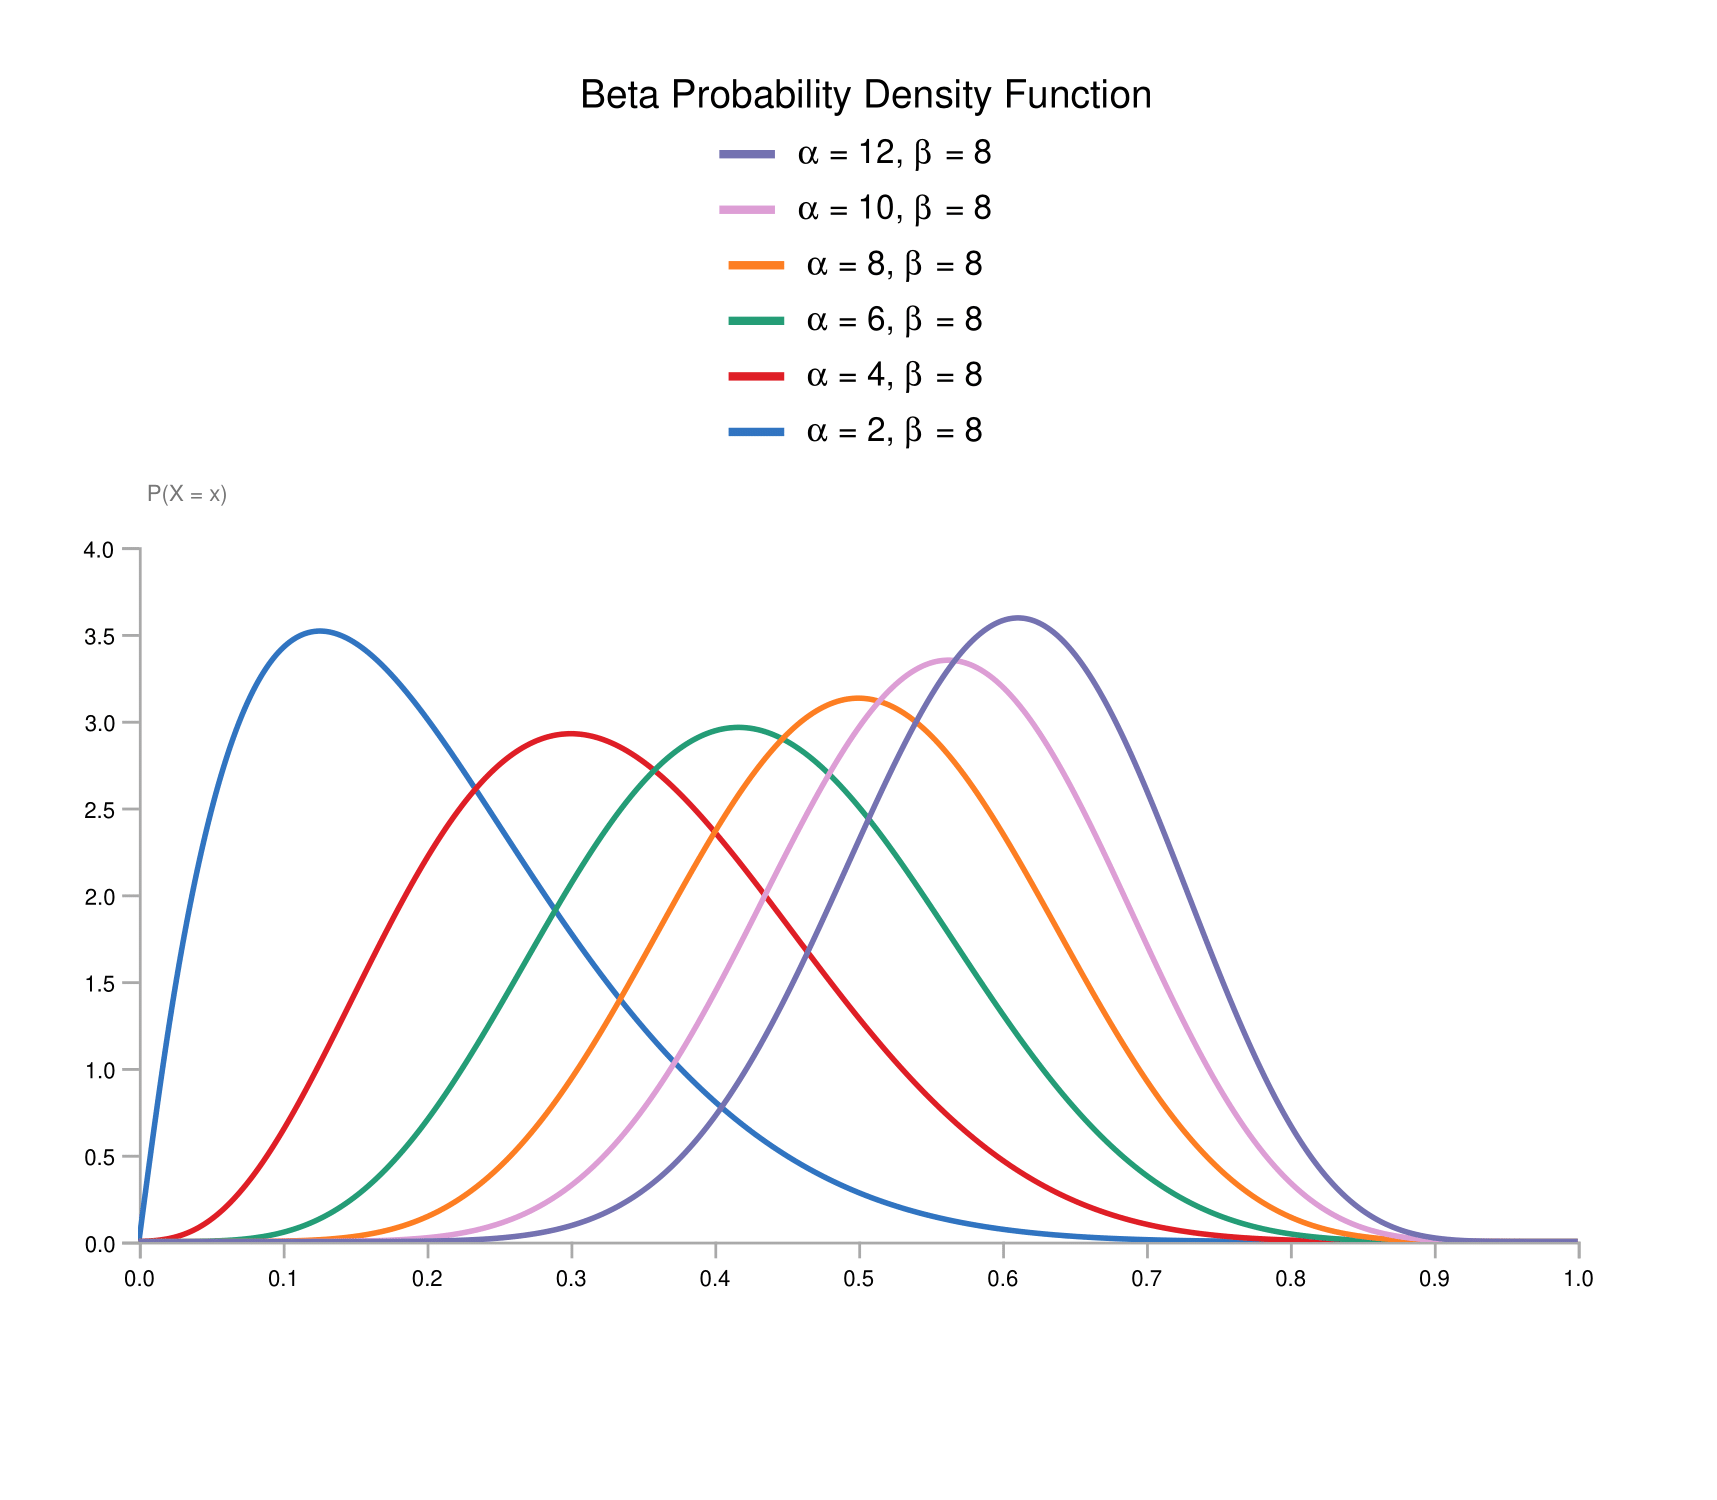
\includegraphics[width=6.26cm]{./images/chart (1)-1.png}\quad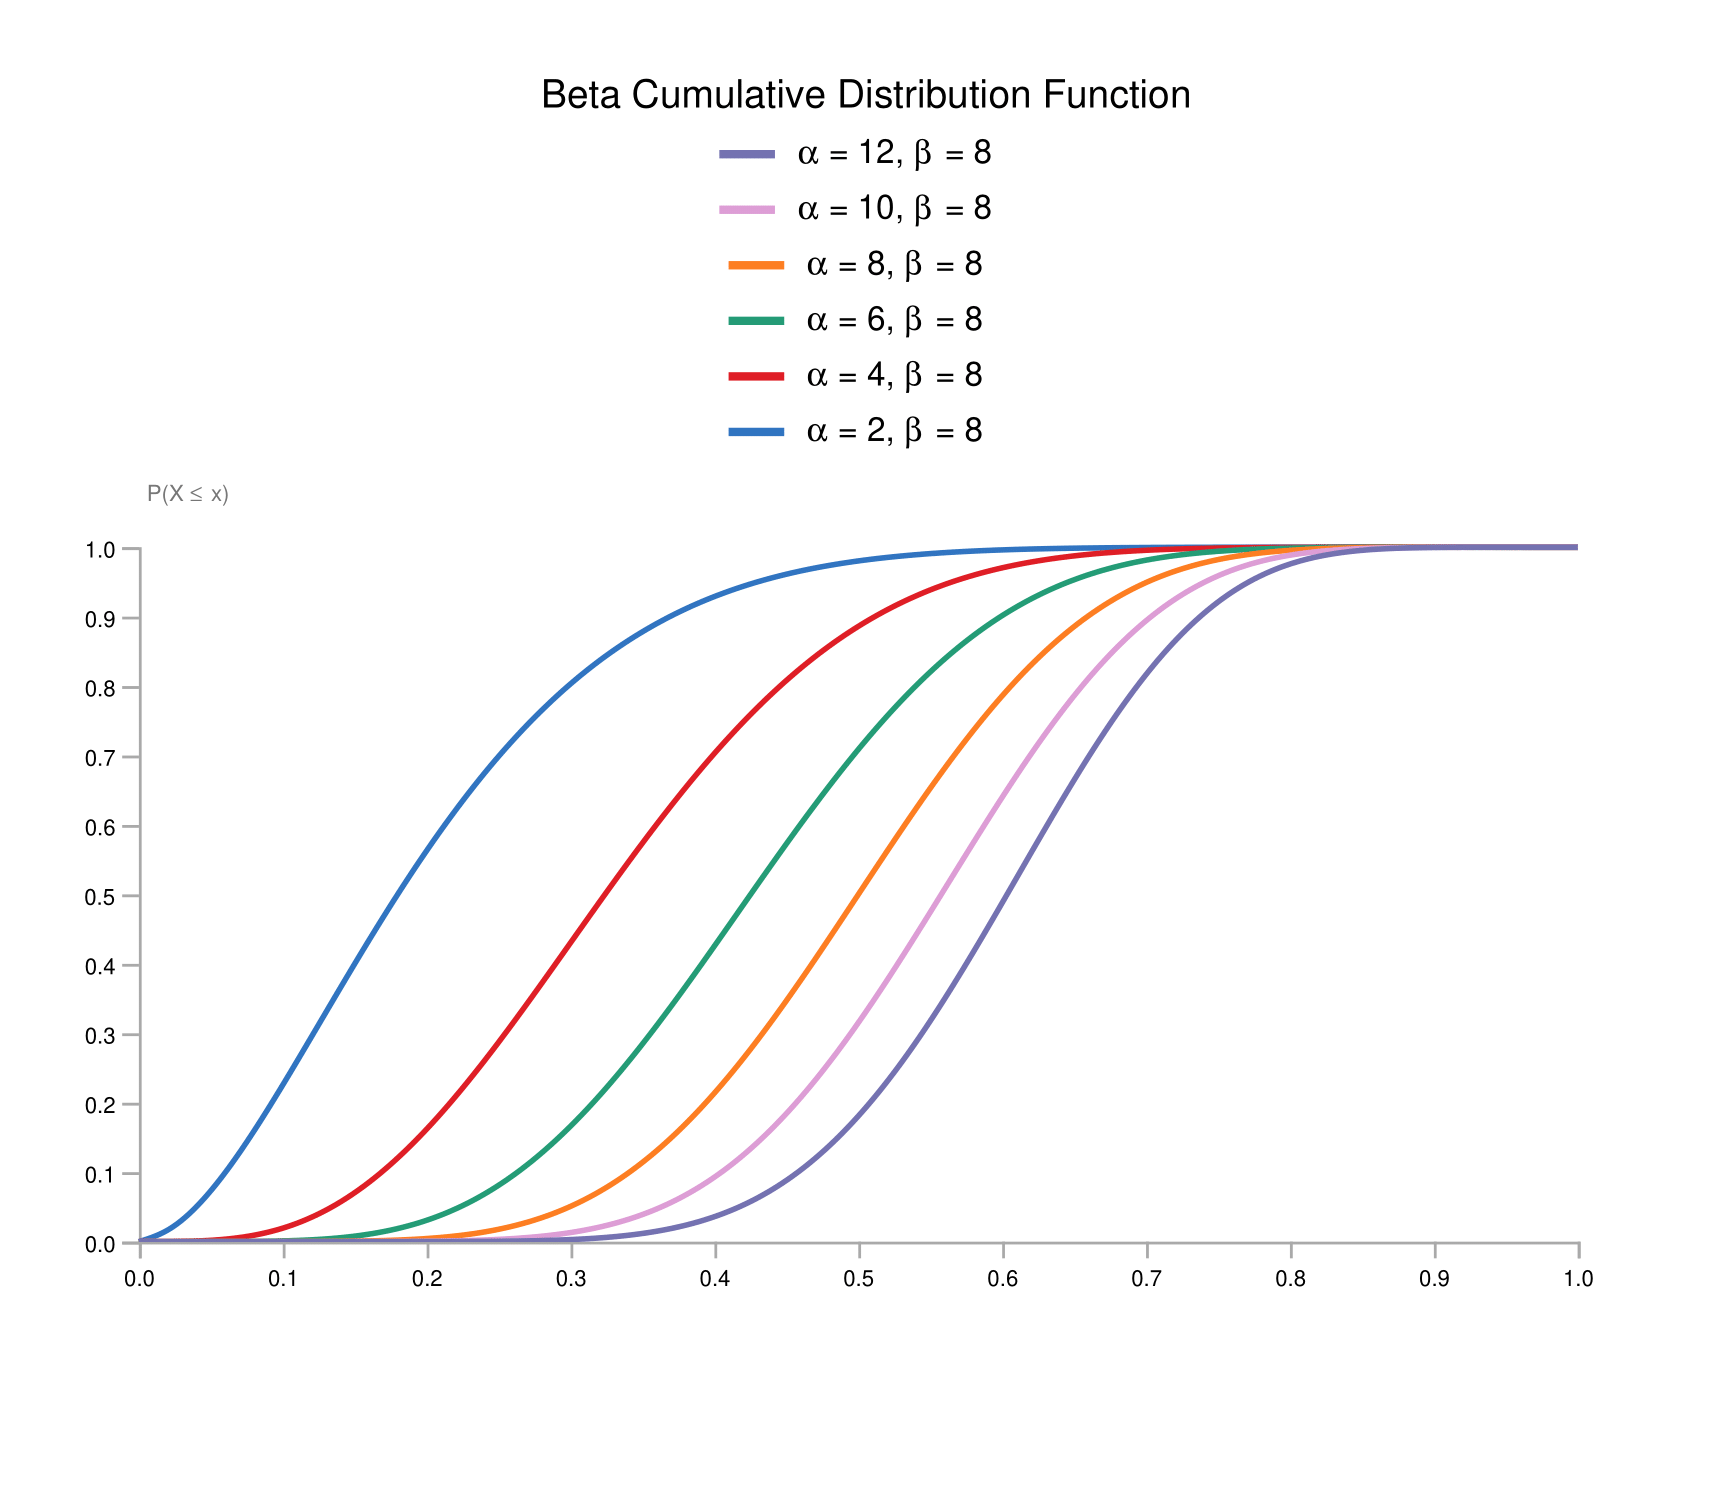
\includegraphics[width=6cm]{./images/chart (2)-1.png}
	\caption{Probability density function and cumulative distribution function of the Beta distributions considered in settings Synthetic B and Synthetic C.}
	\label{beta}
\end{figure}

\subsection{Synthetic C}

In this setting, we model the common situation where high feedback discourage long persistency, as previously discussed in Chapter \ref{CF}. At each time t, the true length $l_{j,t}$ is sampled from a Beta distribution depending on the pulled arm $a_j$. For each arm $a_j$, the feedback is $R_j$ is set such that to higher Beta mean corresponds lower feedback. We set $T_{max}=50,100,150,200$. For each $T_{max}$ adopted, the experiment is repeated for 50 independent runs. The full description of the arms is provided in Table \ref{tabSC} where with $\mu_{T_{max}}$ we indicate the expected pull reward in the configuration where $T_{max}$ is adopted.



\begin{table}[H]
	\centering
	\caption{Description of the arms in setting Synthetic C.}
	
	\begin{tabular}{|c|cccccc|}
		\hline
		\textbf{Arm}          & $a_0$ & $a_1$ & $a_2$ & $a_3$ & $a_4$ & $a_5$ \\ \hline
		\textbf{R}            & 6     & 5     & 4     & 3     & 2     & 1     \\
		$\boldsymbol{\alpha}$ & 2     & 4     & 6     & 8     & 10    & 12    \\
		$\boldsymbol{\beta}$  & 8     & 8     & 8     & 8     & 8     & 8     \\
		$\boldsymbol{\mu_{50}}$    & 10.50 & 17.17 & 21.93 & 25.50 & 28.28 & 30.3  \\ 
		$\boldsymbol{\mu_{100}}$    & 10.50 & 17.17 & 21.93 & 25.50 & 28.28 & 30.3  \\ 
		$\boldsymbol{\mu_{150}}$    & 10.50 & 17.17 & 21.93 & 25.50 & 28.28 & 30.3  \\ 
		$\boldsymbol{\mu_{200}}$    & 10.50 & 17.17 & 21.93 & 25.50 & 28.28 & 30.3  \\ \hline
	\end{tabular}
	
	\label{tabSC}
\end{table}

\section{Results}

\begin{figure}[H]
	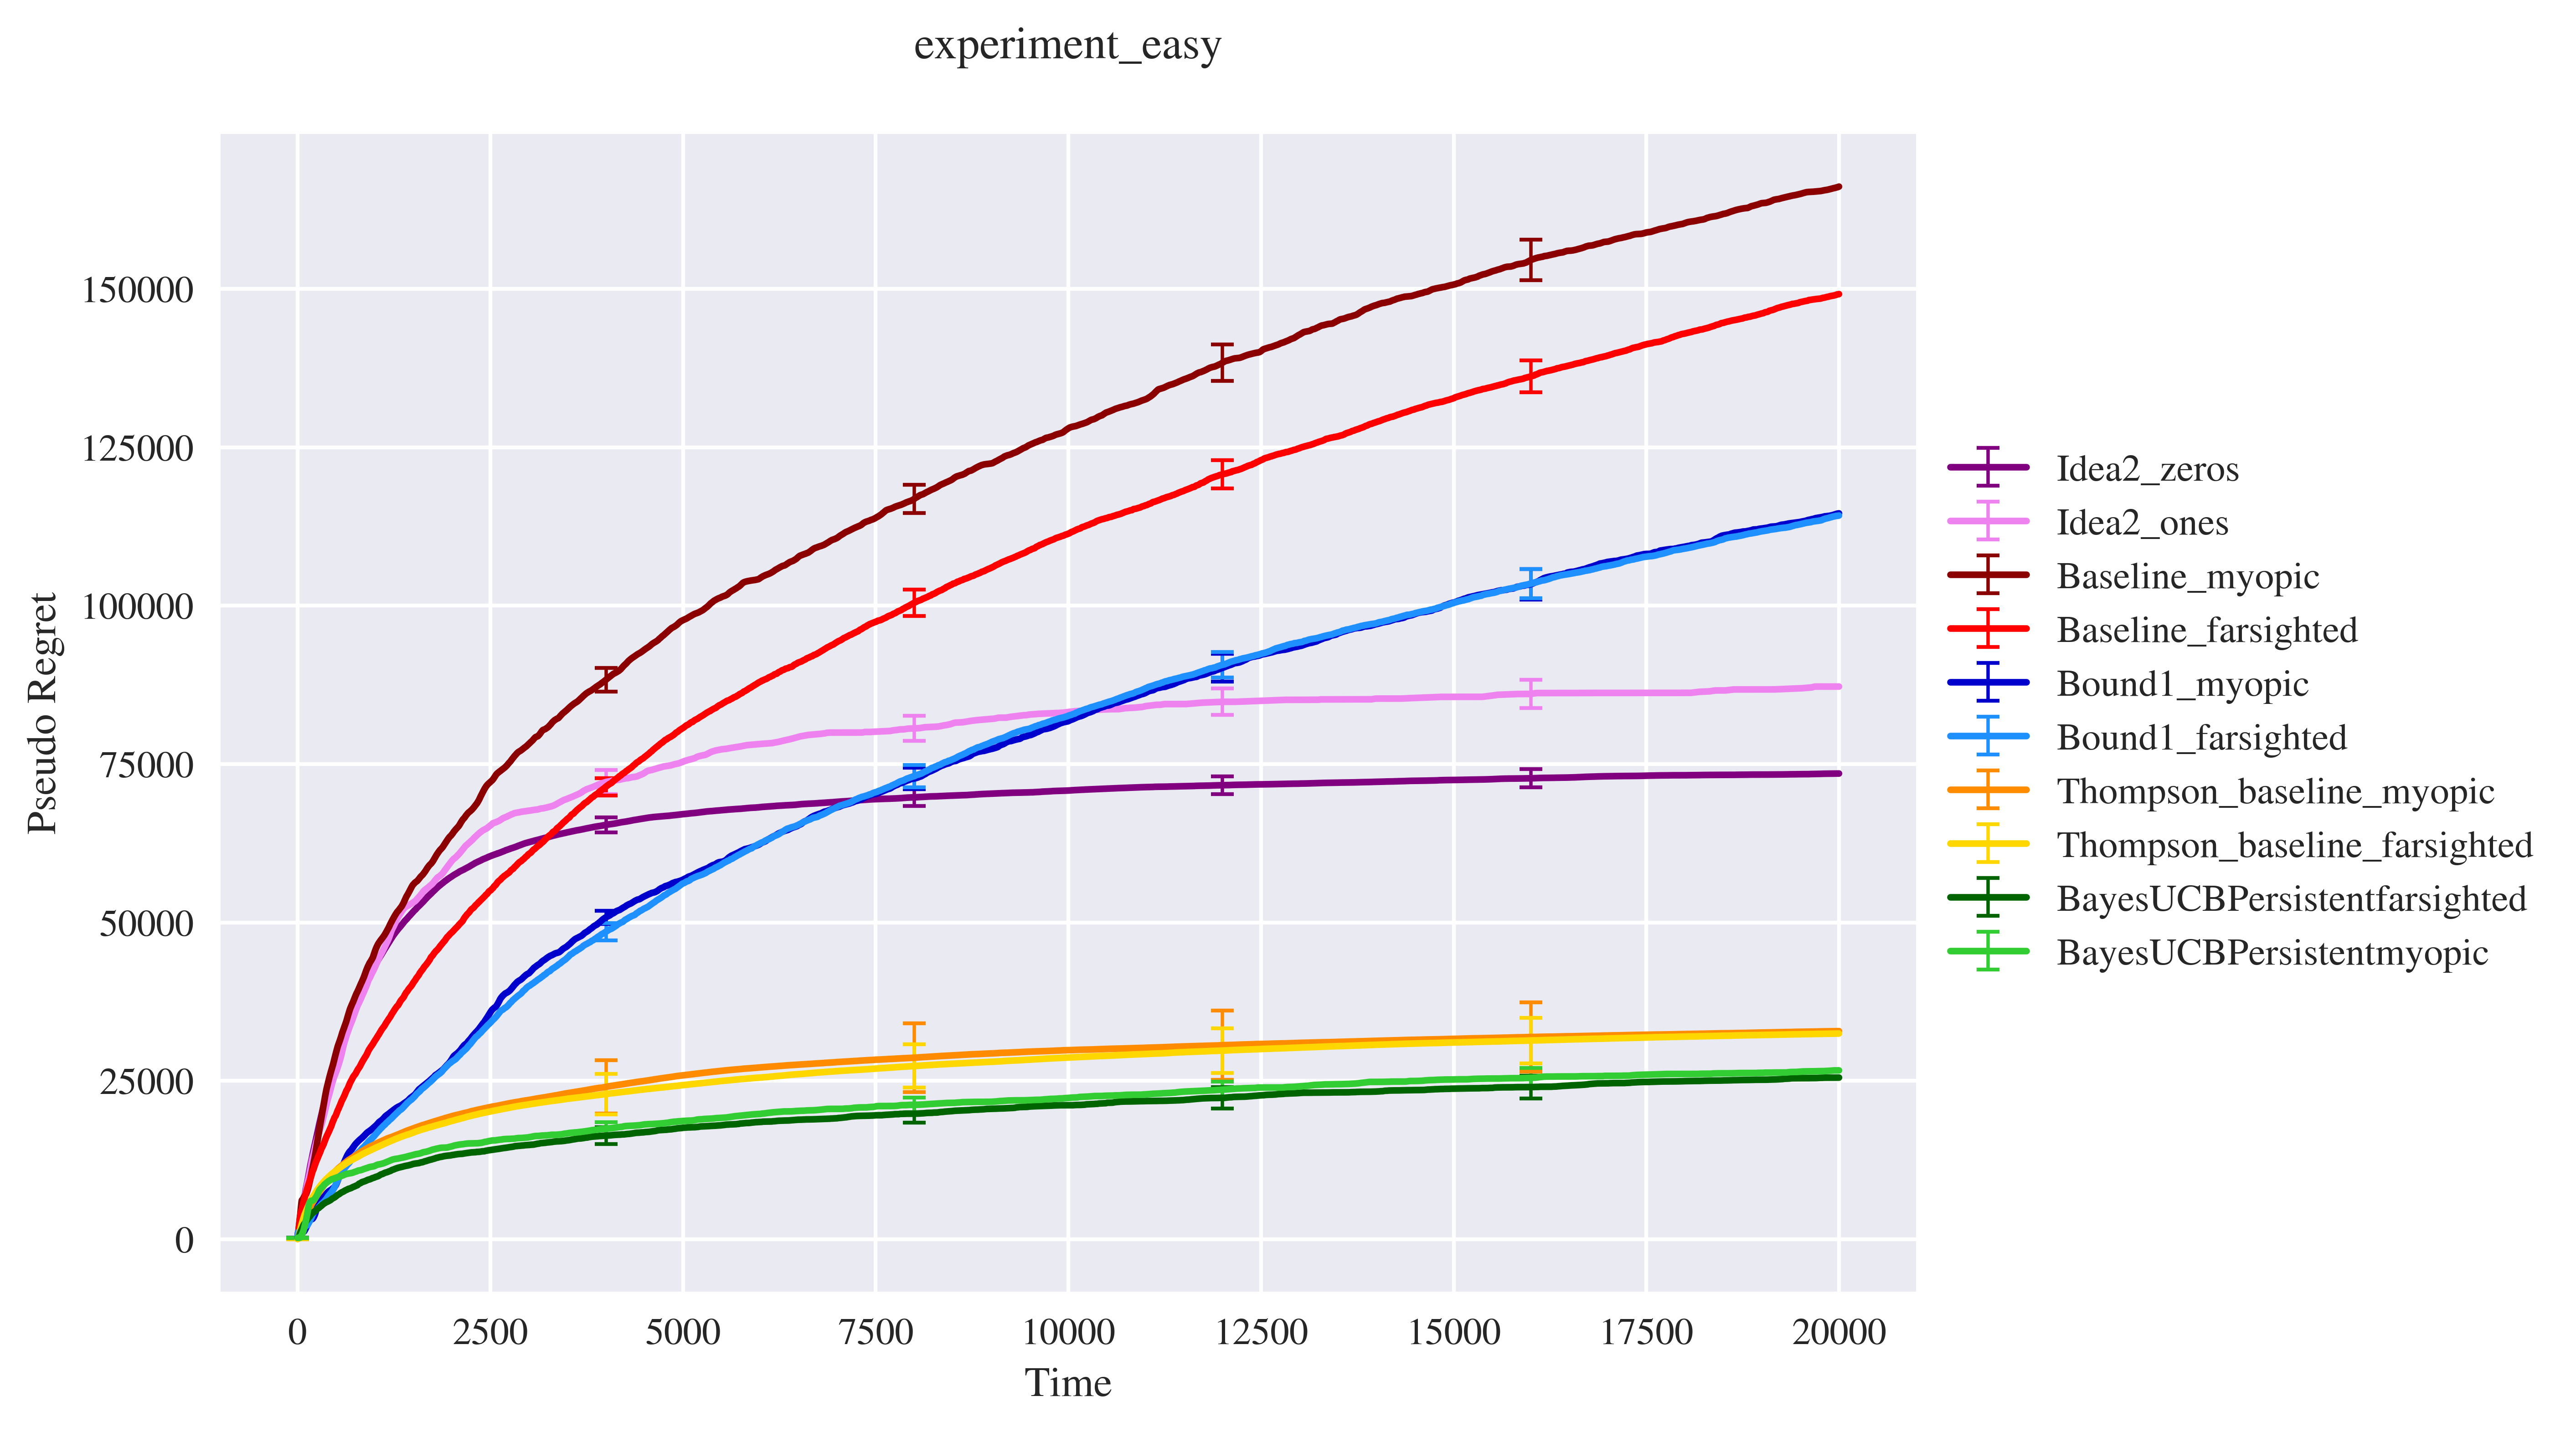
\includegraphics[width=16cm]{./images/experiment_easy ANALYTICS.png}
	\centering	
	\caption{Pseudo regret plot of the experiment Synthetic A.}
\end{figure}
\begin{figure}[H]
	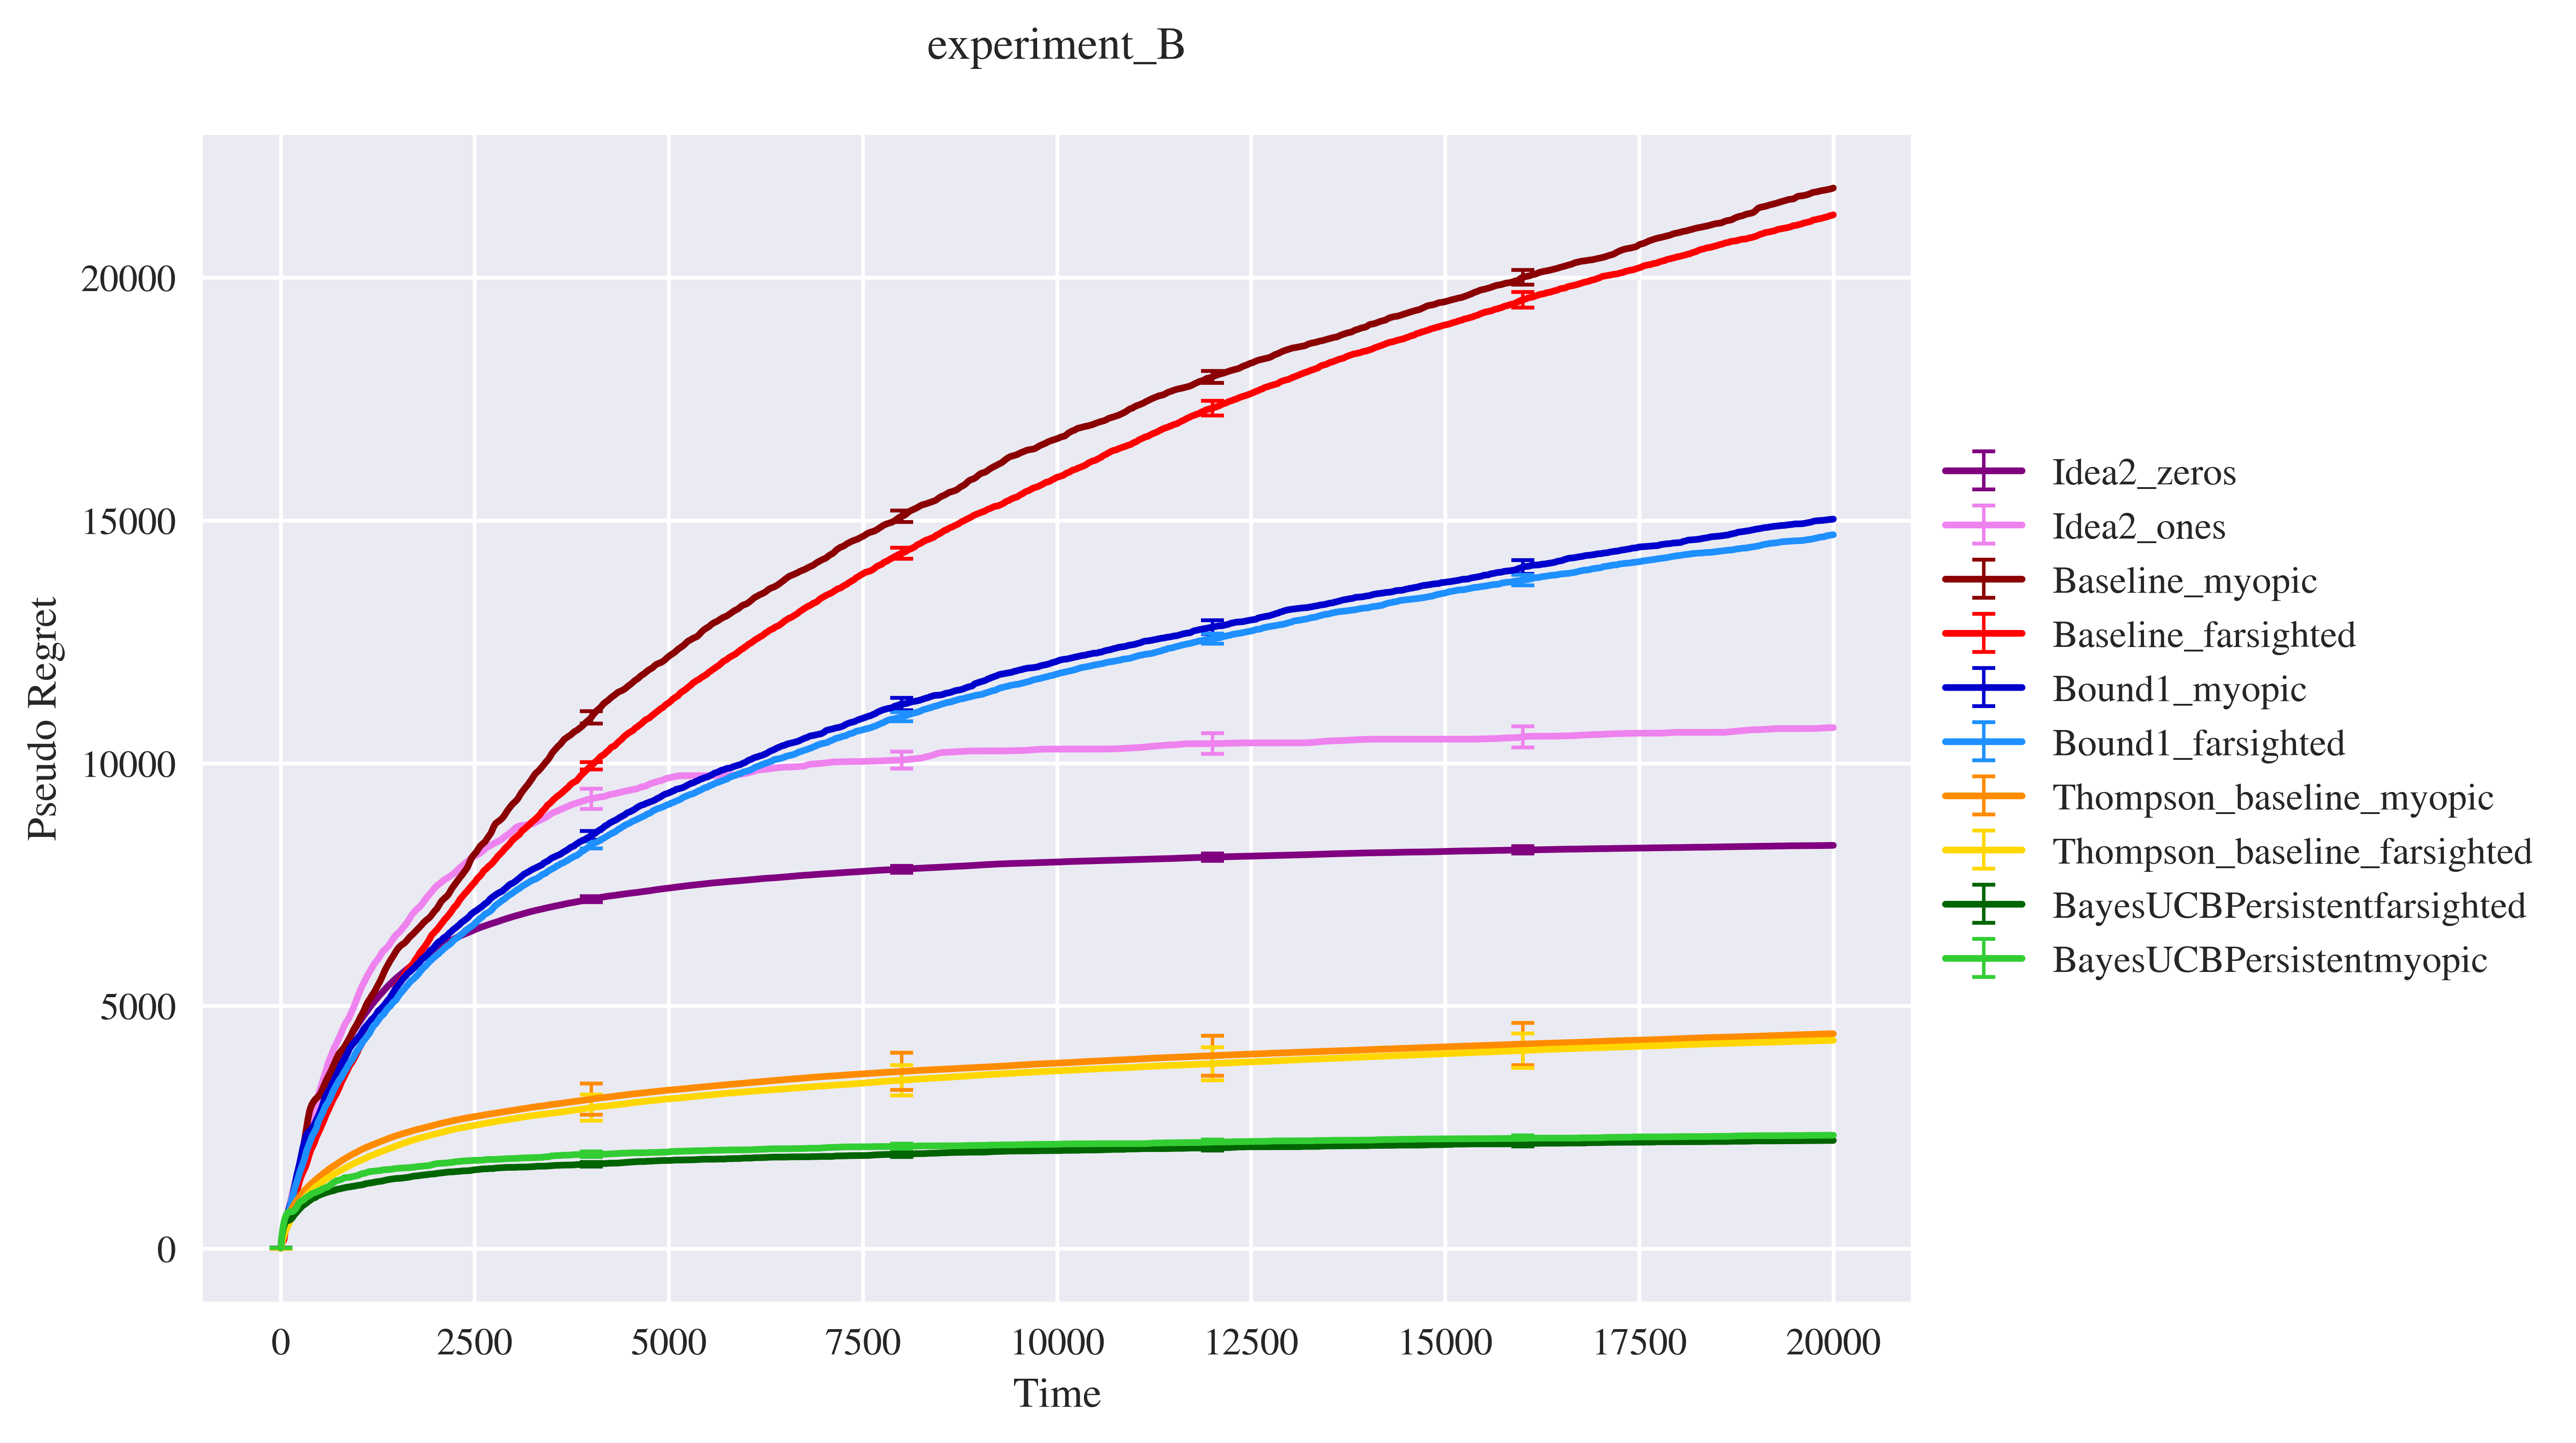
\includegraphics[width=16cm]{./images/experiment_B ANALYTICS.png}
	\centering	
	\caption{Pseudo regret plot of the experiment Synthetic B. }
\end{figure}

\begin{figure}[H]
	\centering
	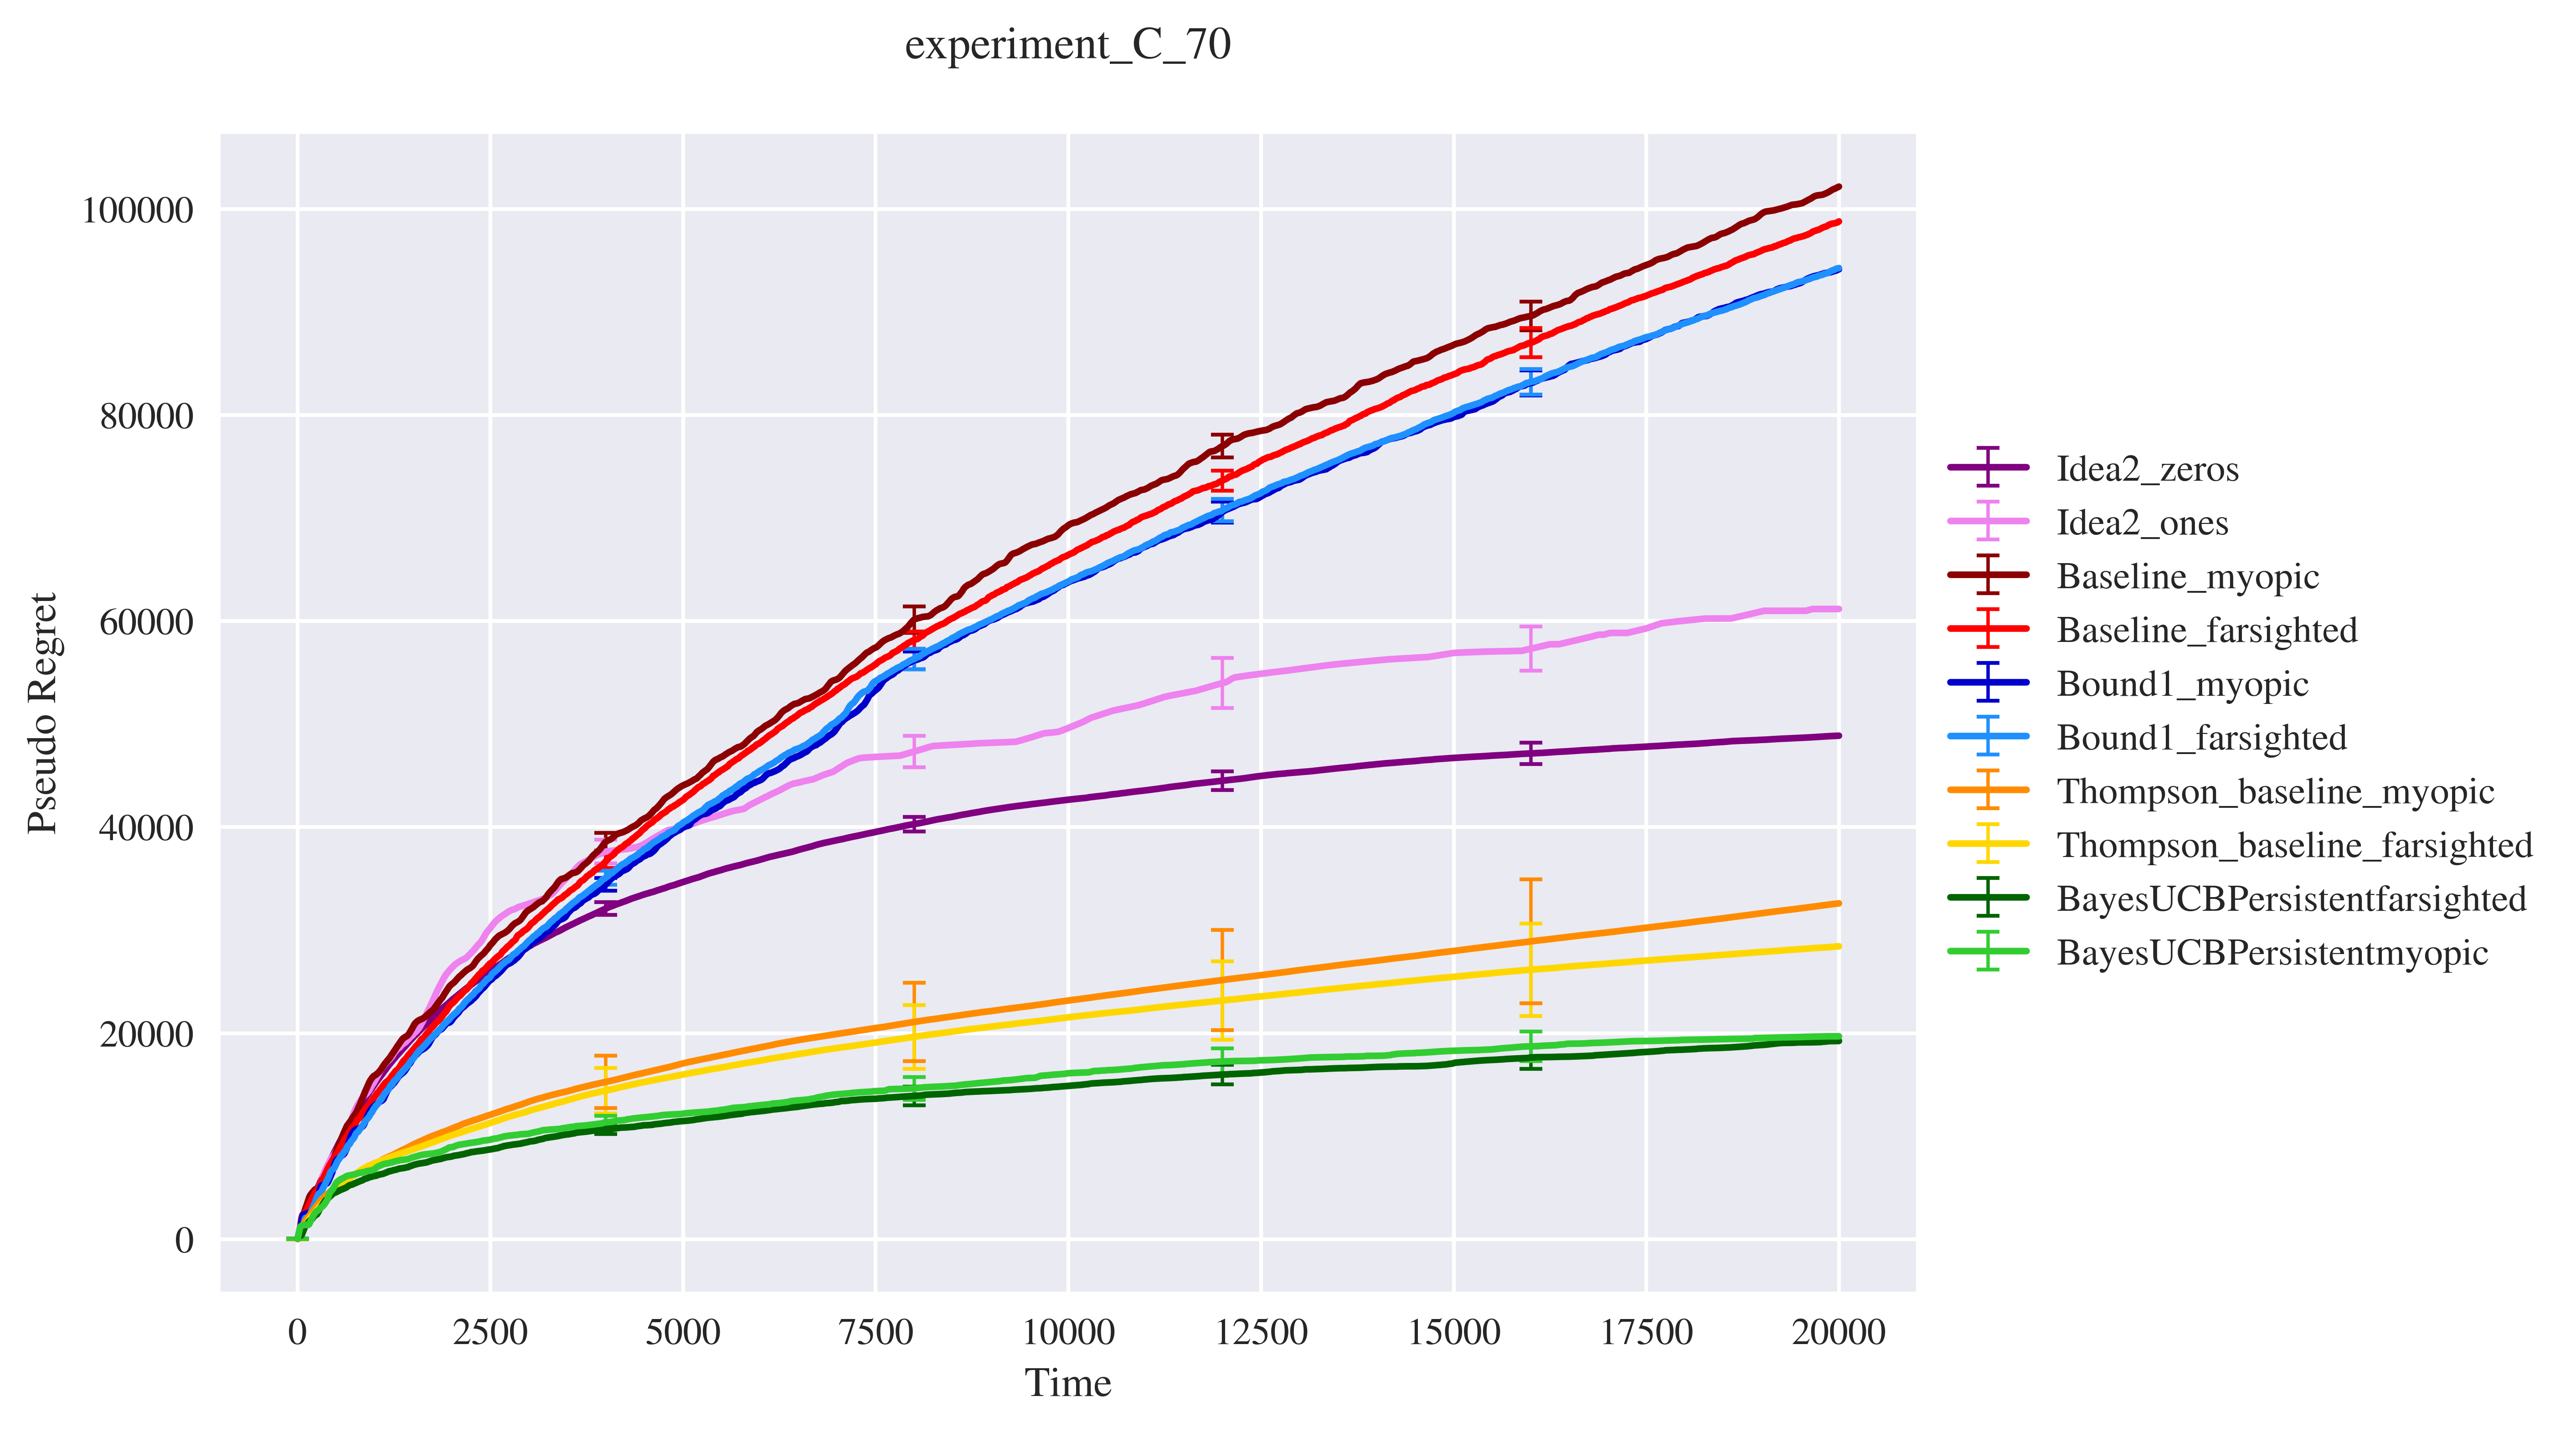
\includegraphics[width=9.5cm]{./images/C/experiment_C_70 ANALYTICS.png}\quad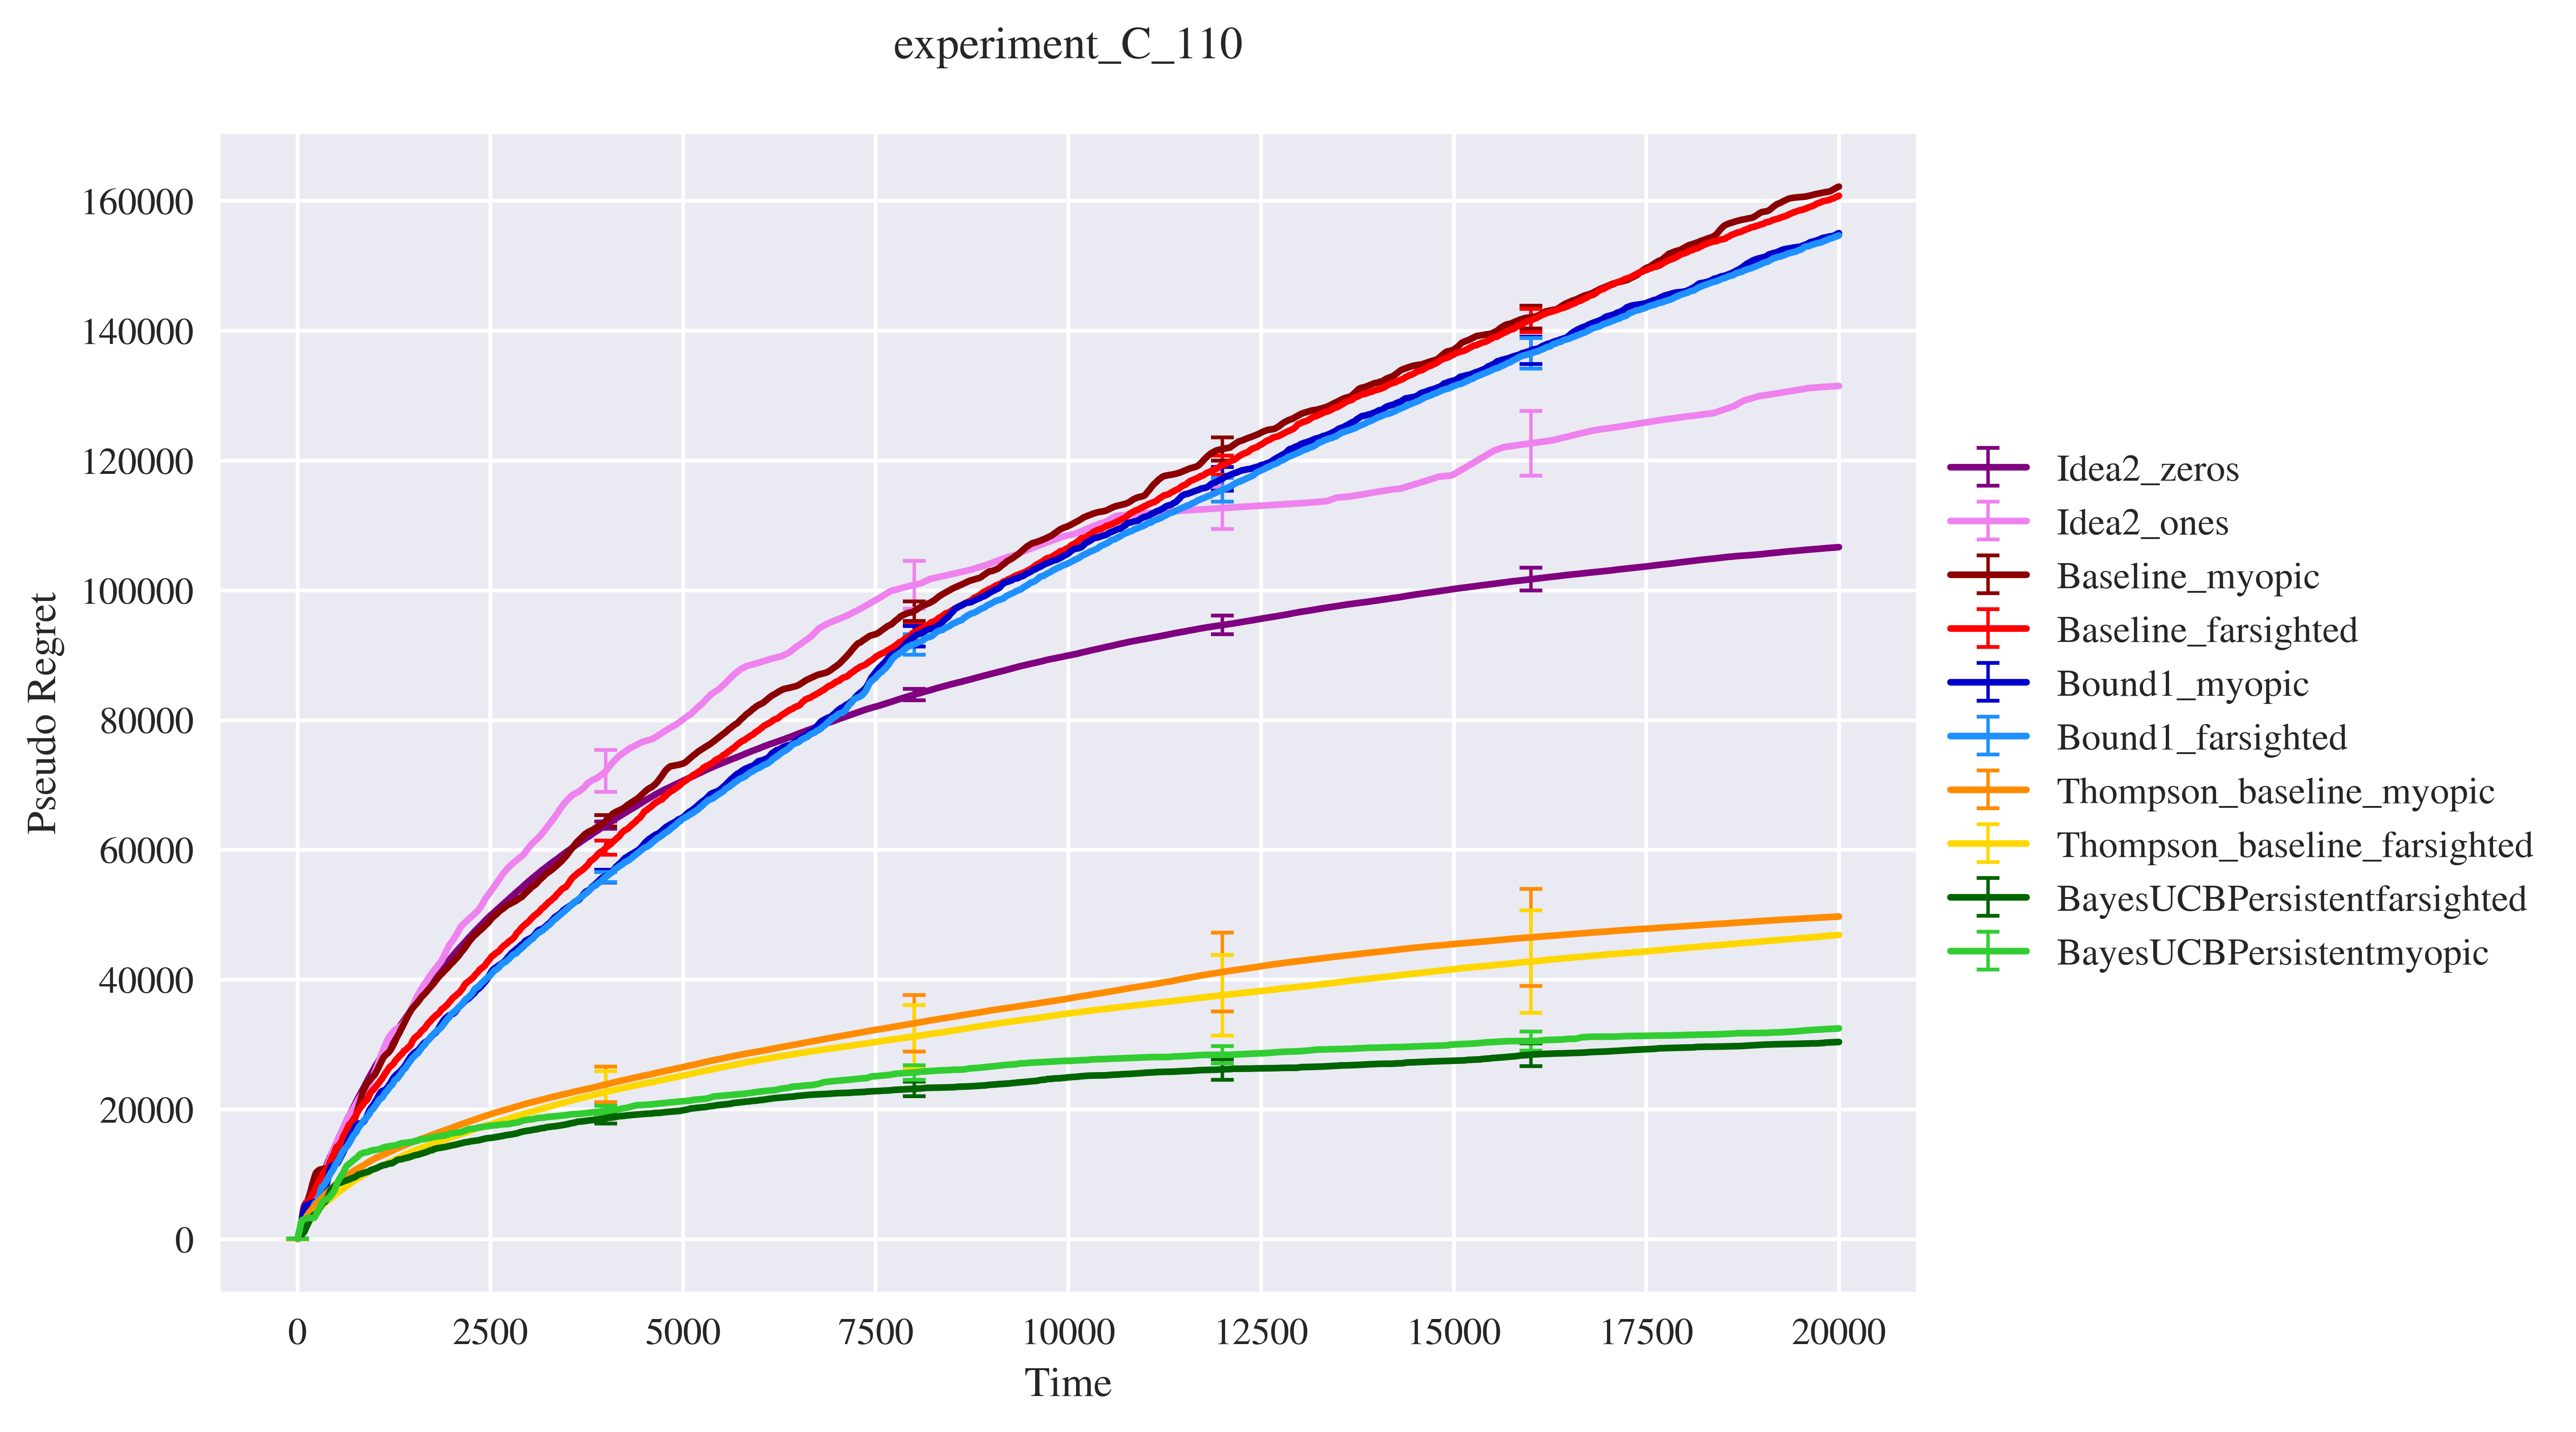
\includegraphics[width=9.5cm]{./images/C/experiment_C_110 ANALYTICS.png}
	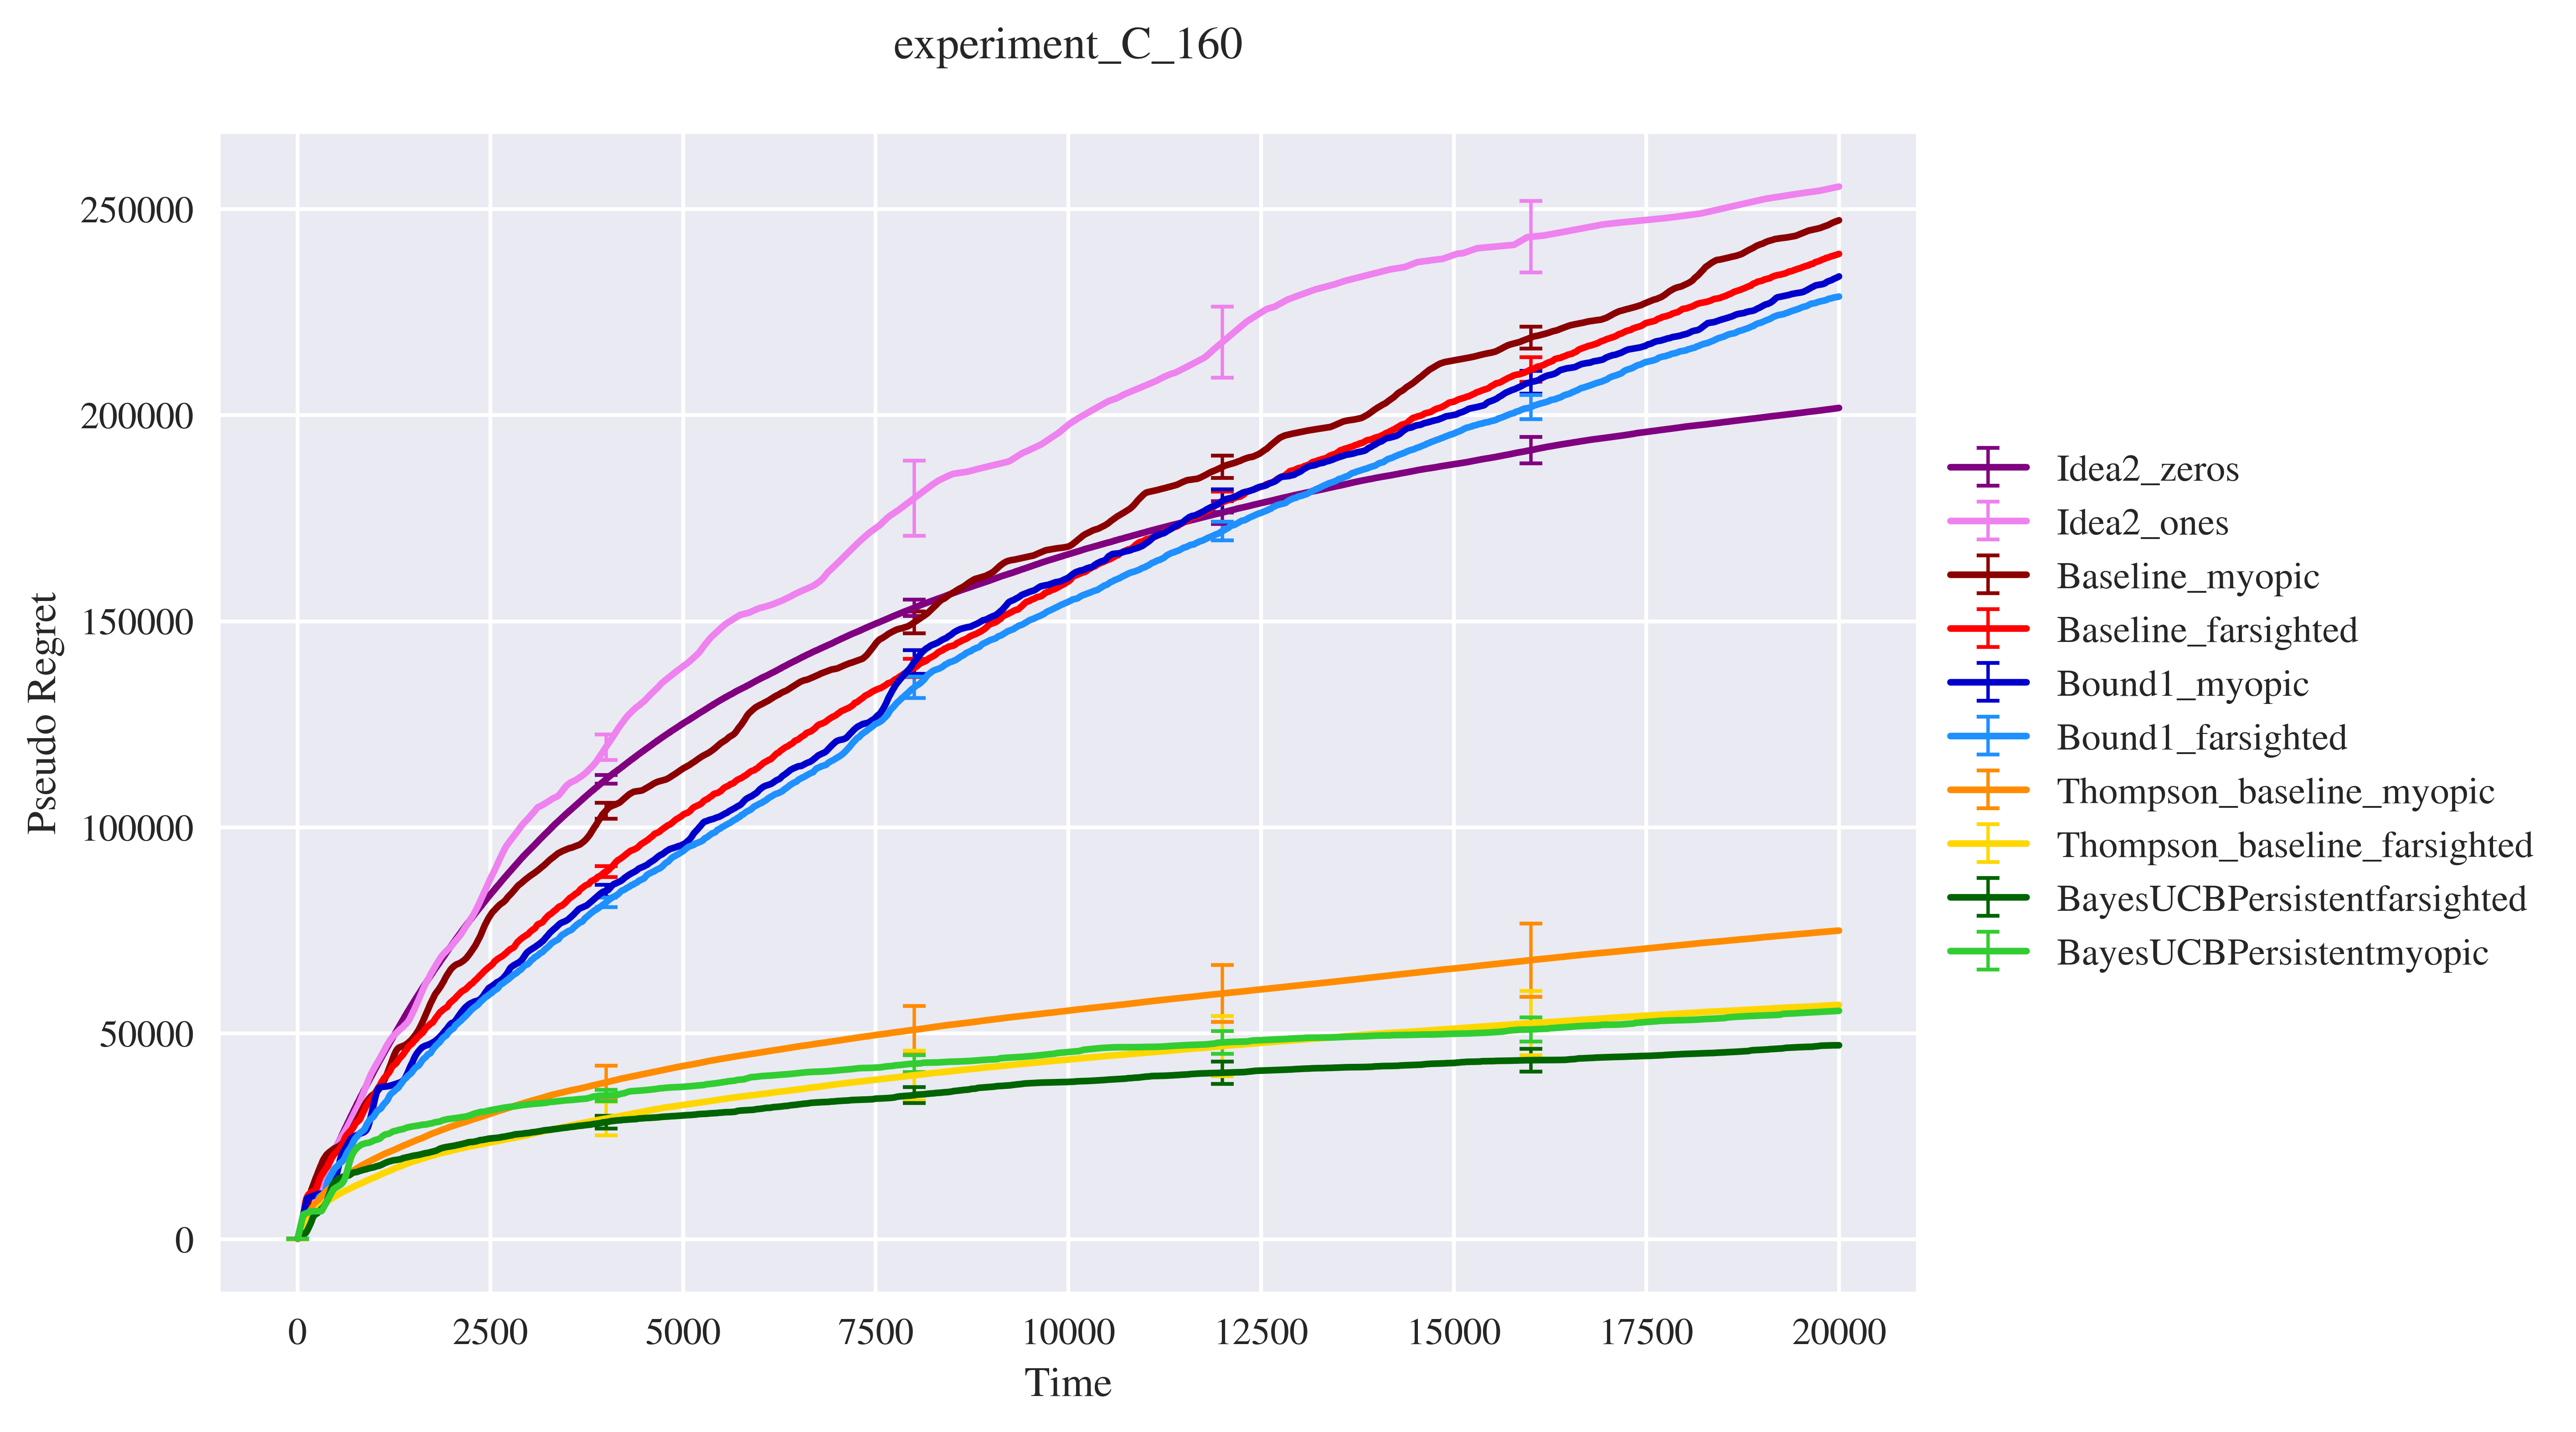
\includegraphics[width=9.5cm]{./images/C/experiment_C_160 ANALYTICS.png}\quad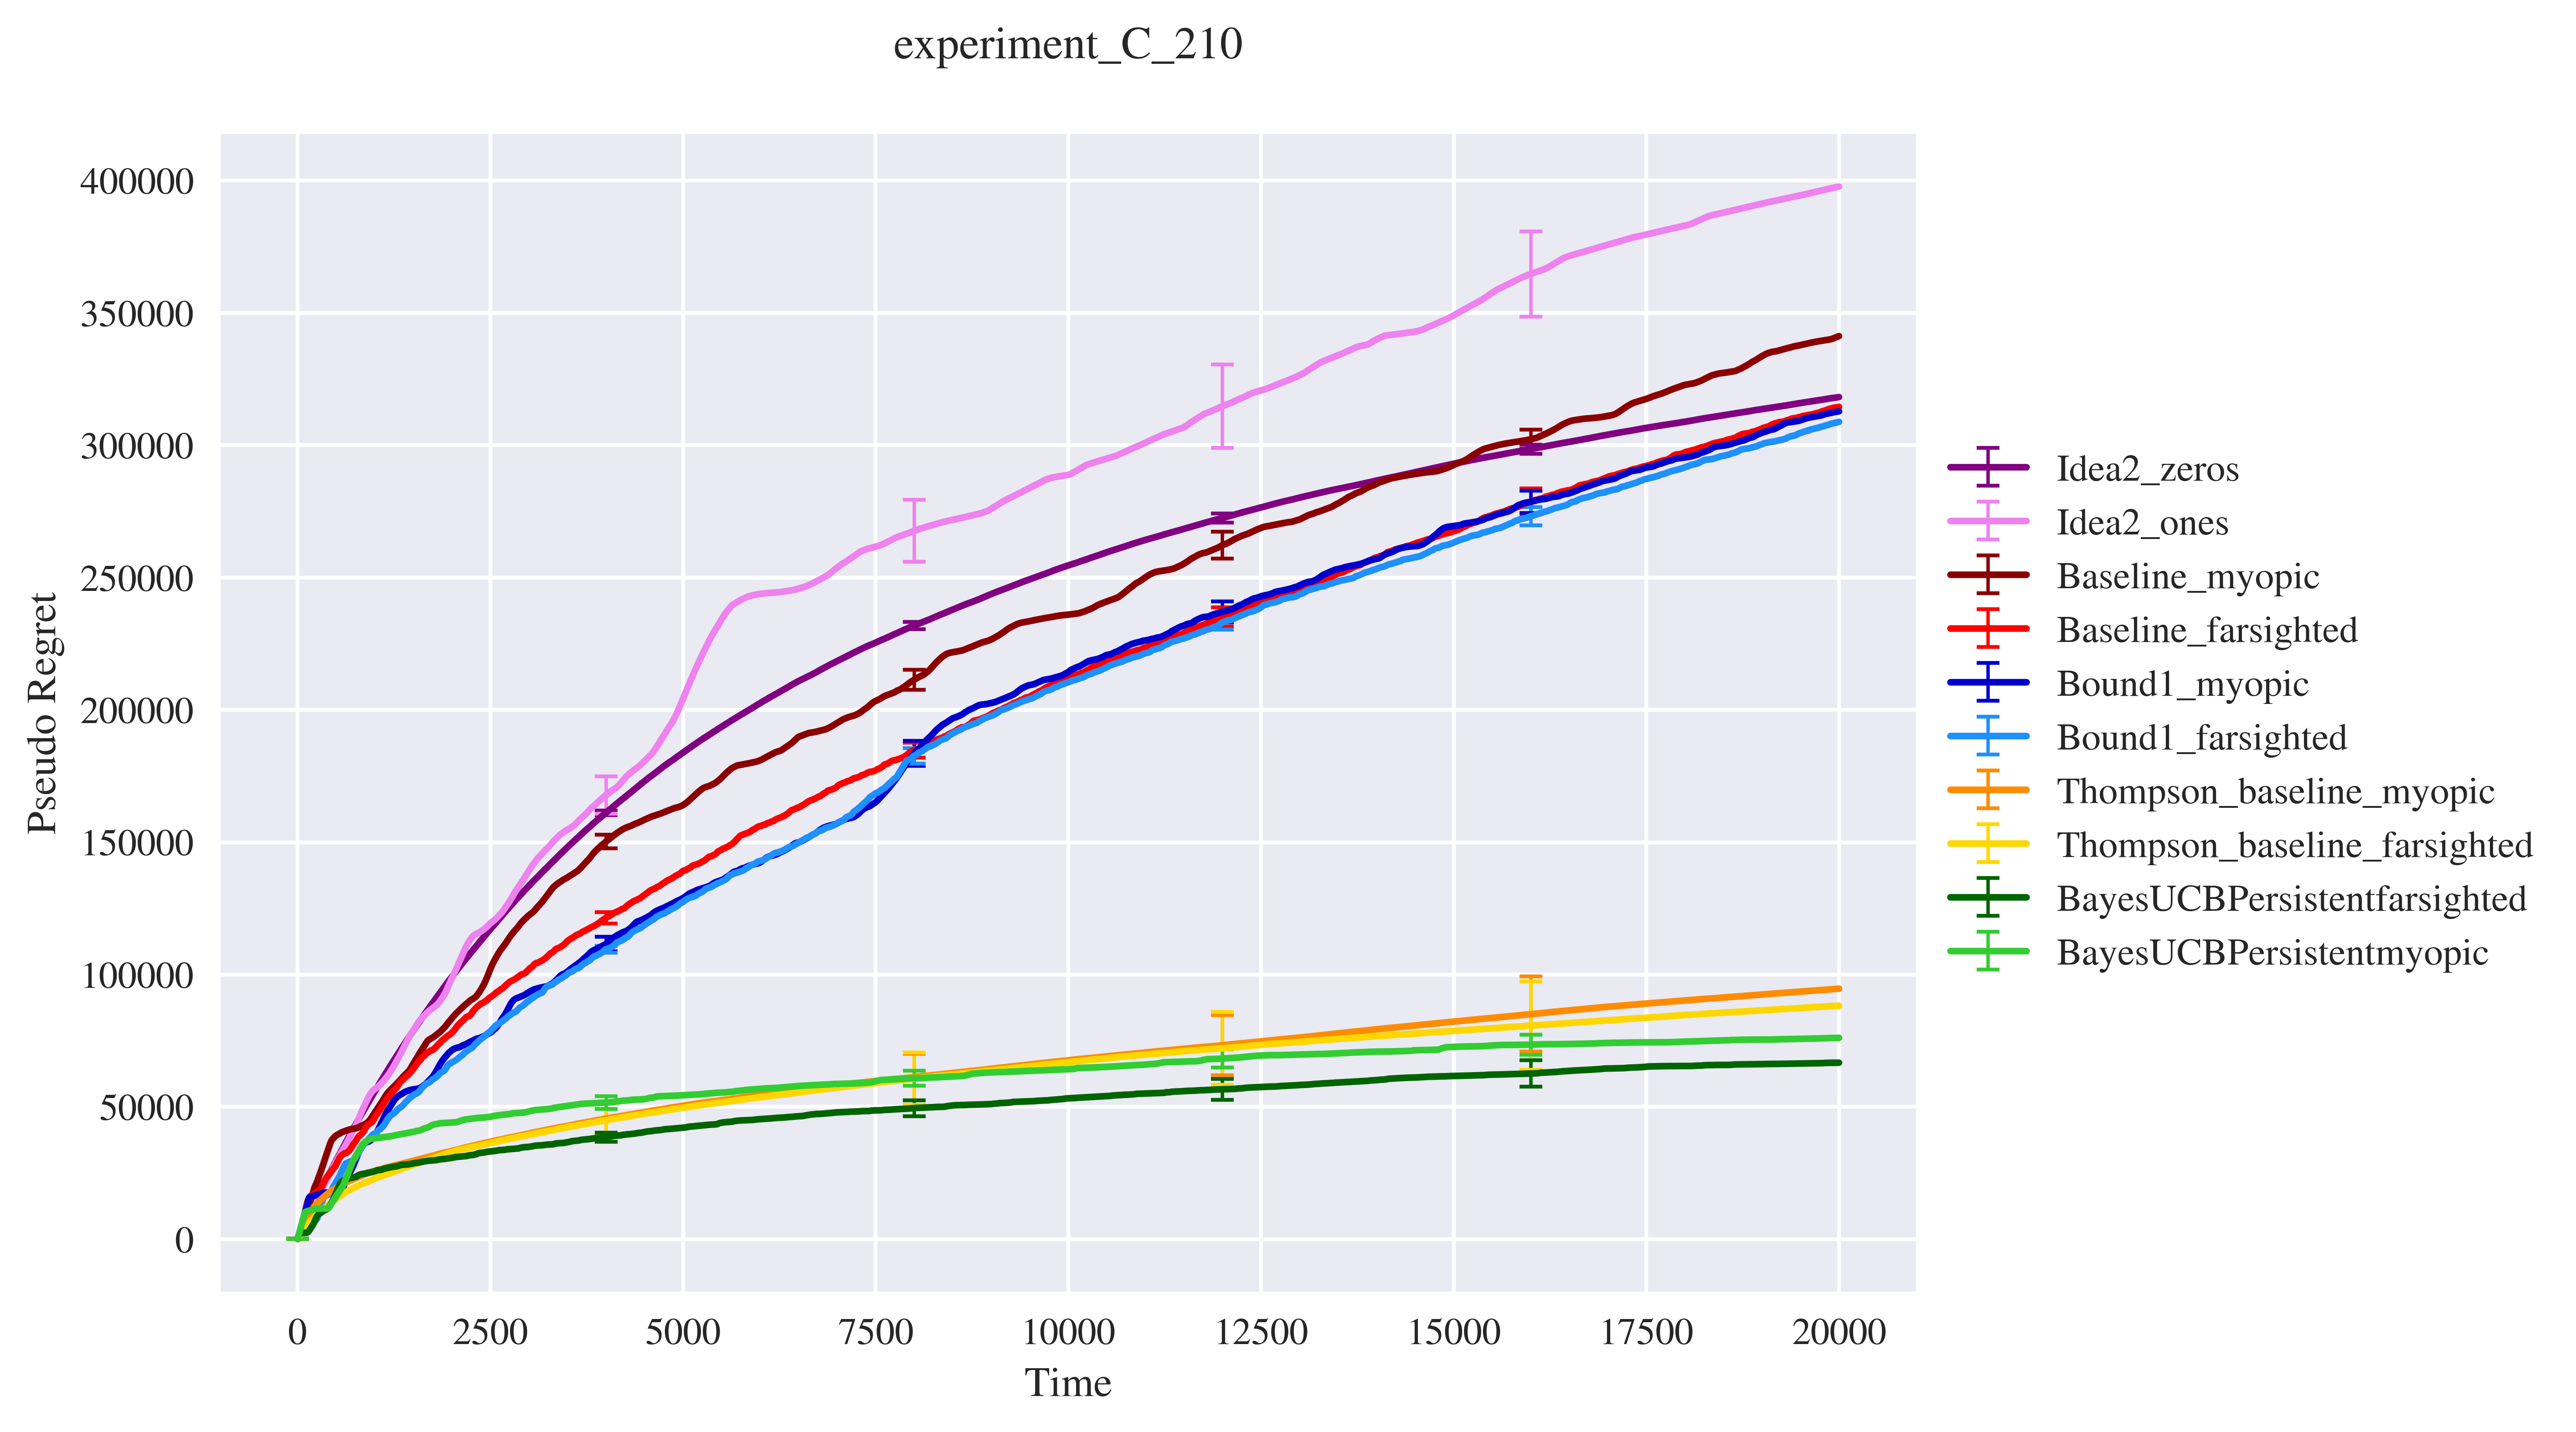
\includegraphics[width=9.5cm]{./images/C/experiment_C_210 ANALYTICS.png}
	\caption{Pseudo regret plot of the experiment Synthetic C.}
	
\end{figure}

%SPOTIFY

\begin{figure}[H]
	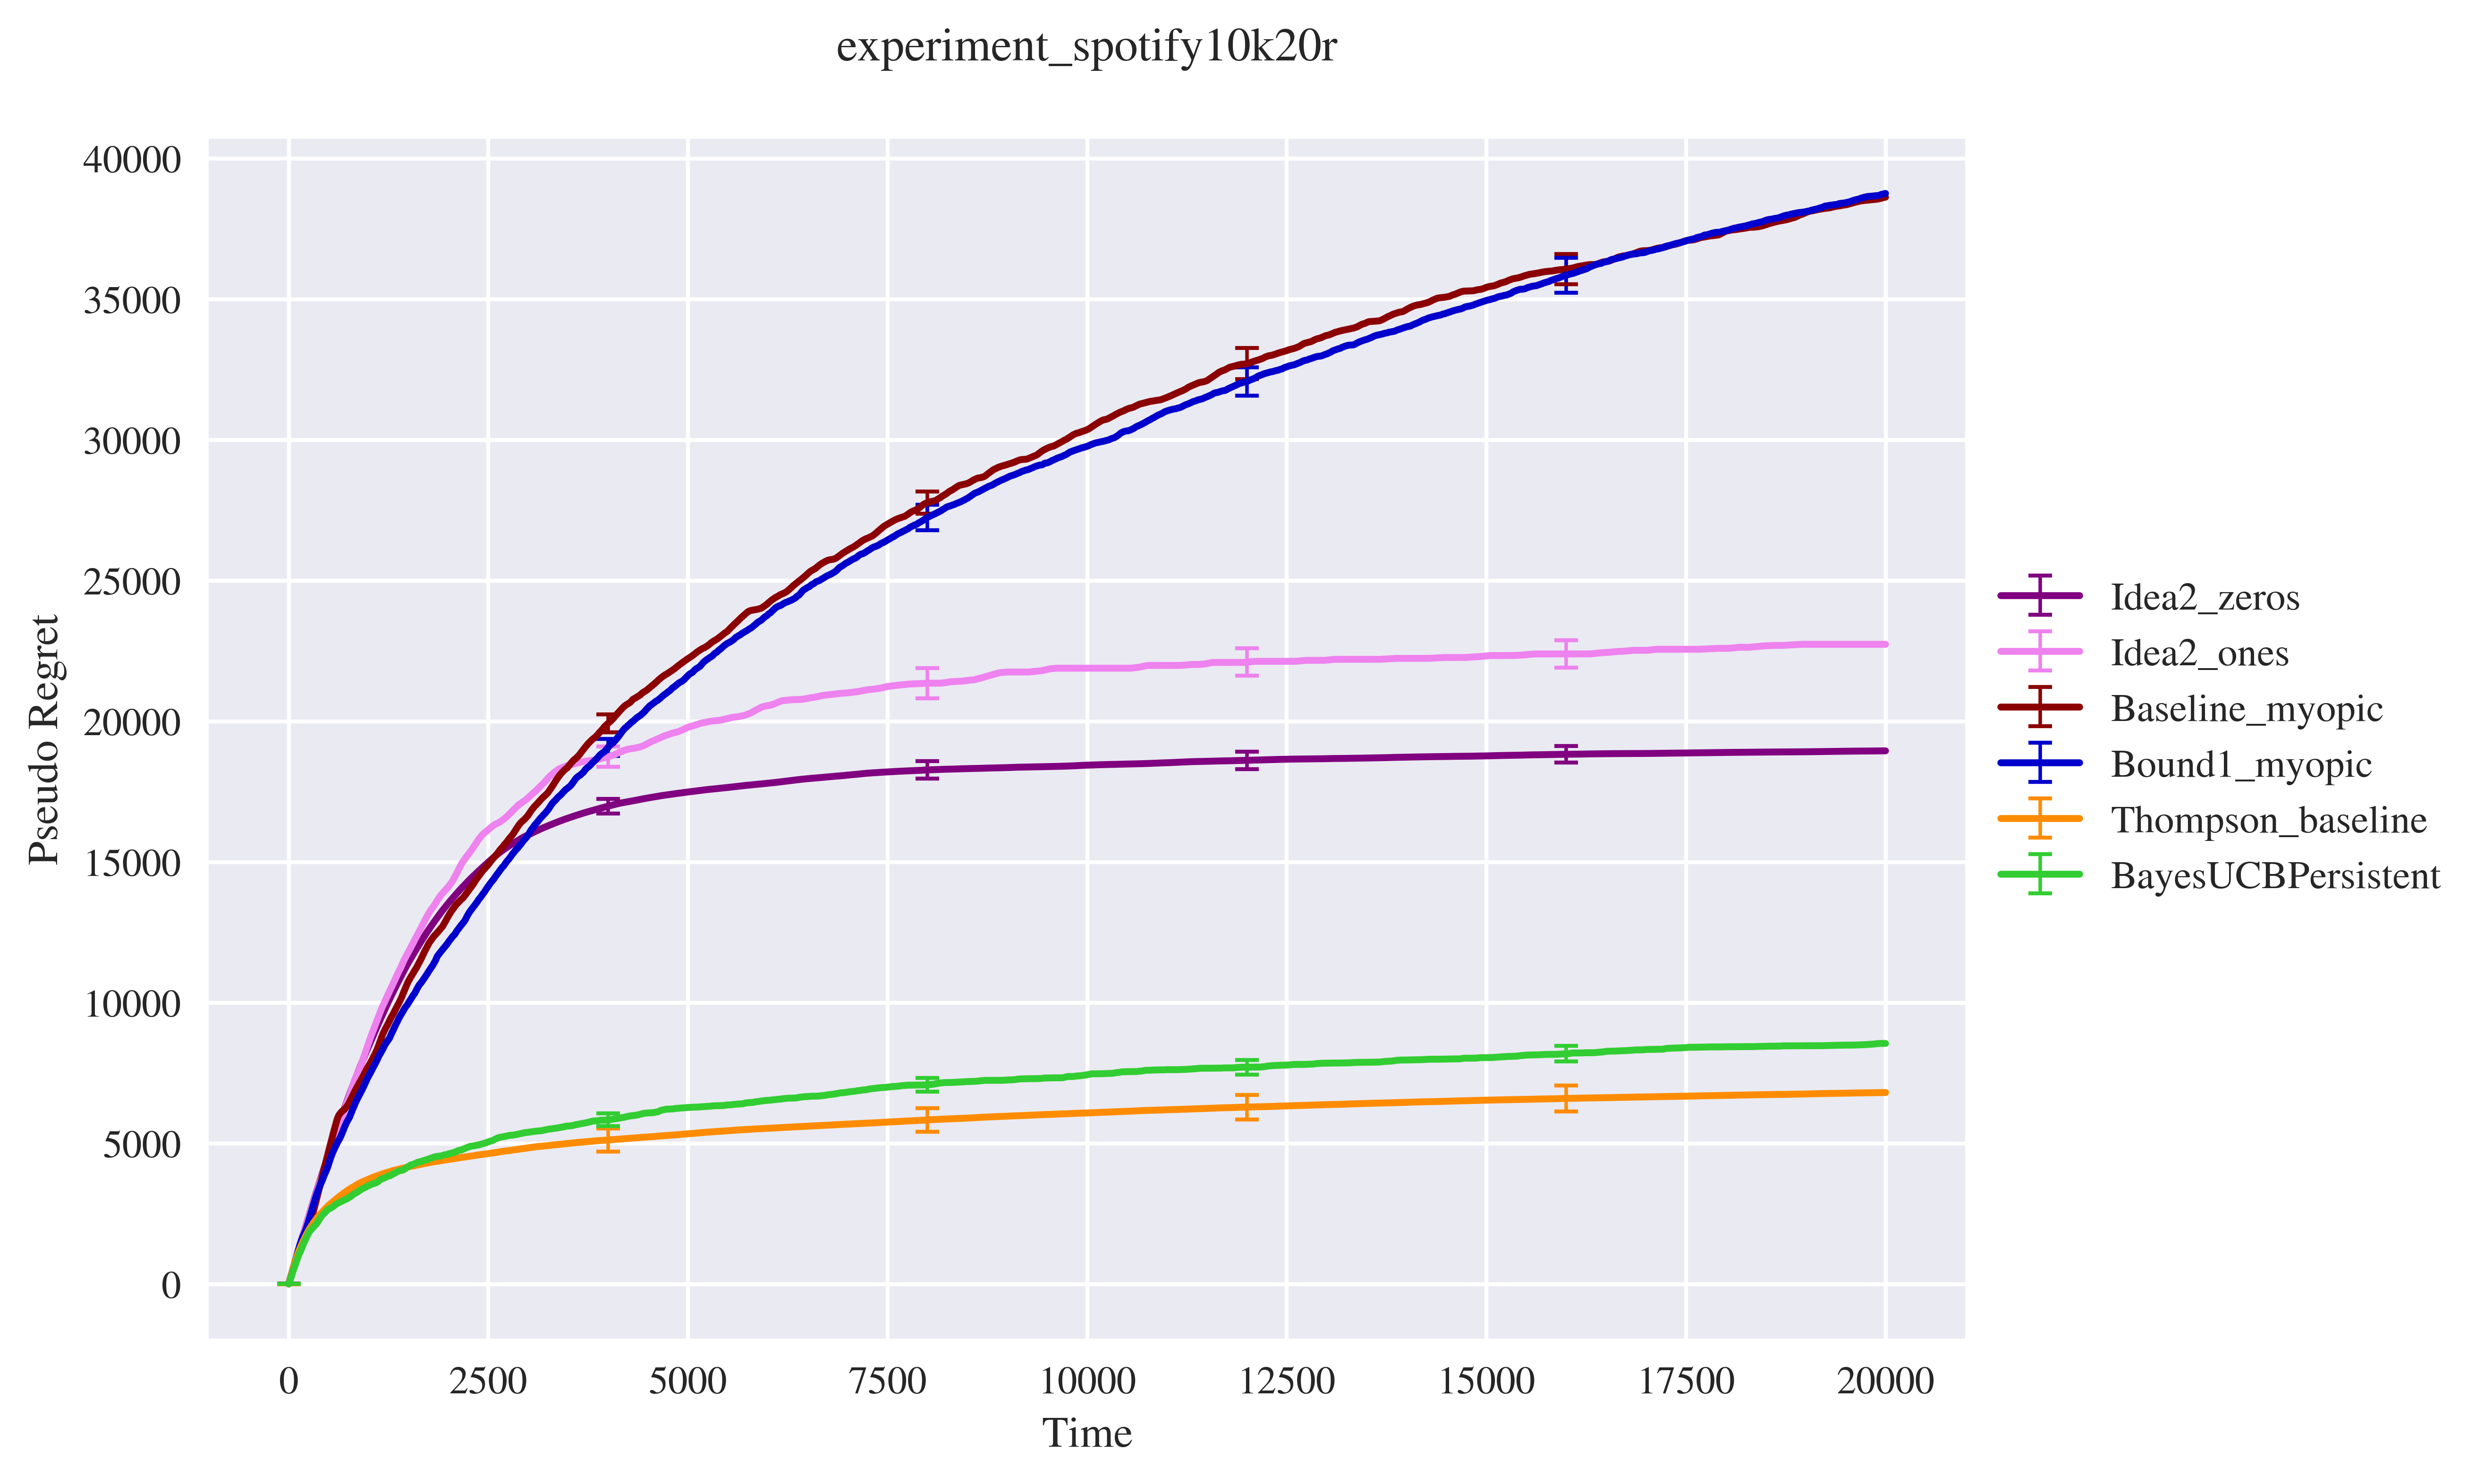
\includegraphics[width=16cm]{./images/experiment_spotify10k20r ANALYTICS.png}
	\centering	
	\caption{Pseudo regret plot of the experiment Spotify Playlist Problem.}
\end{figure}

\begin{figure}[H]
	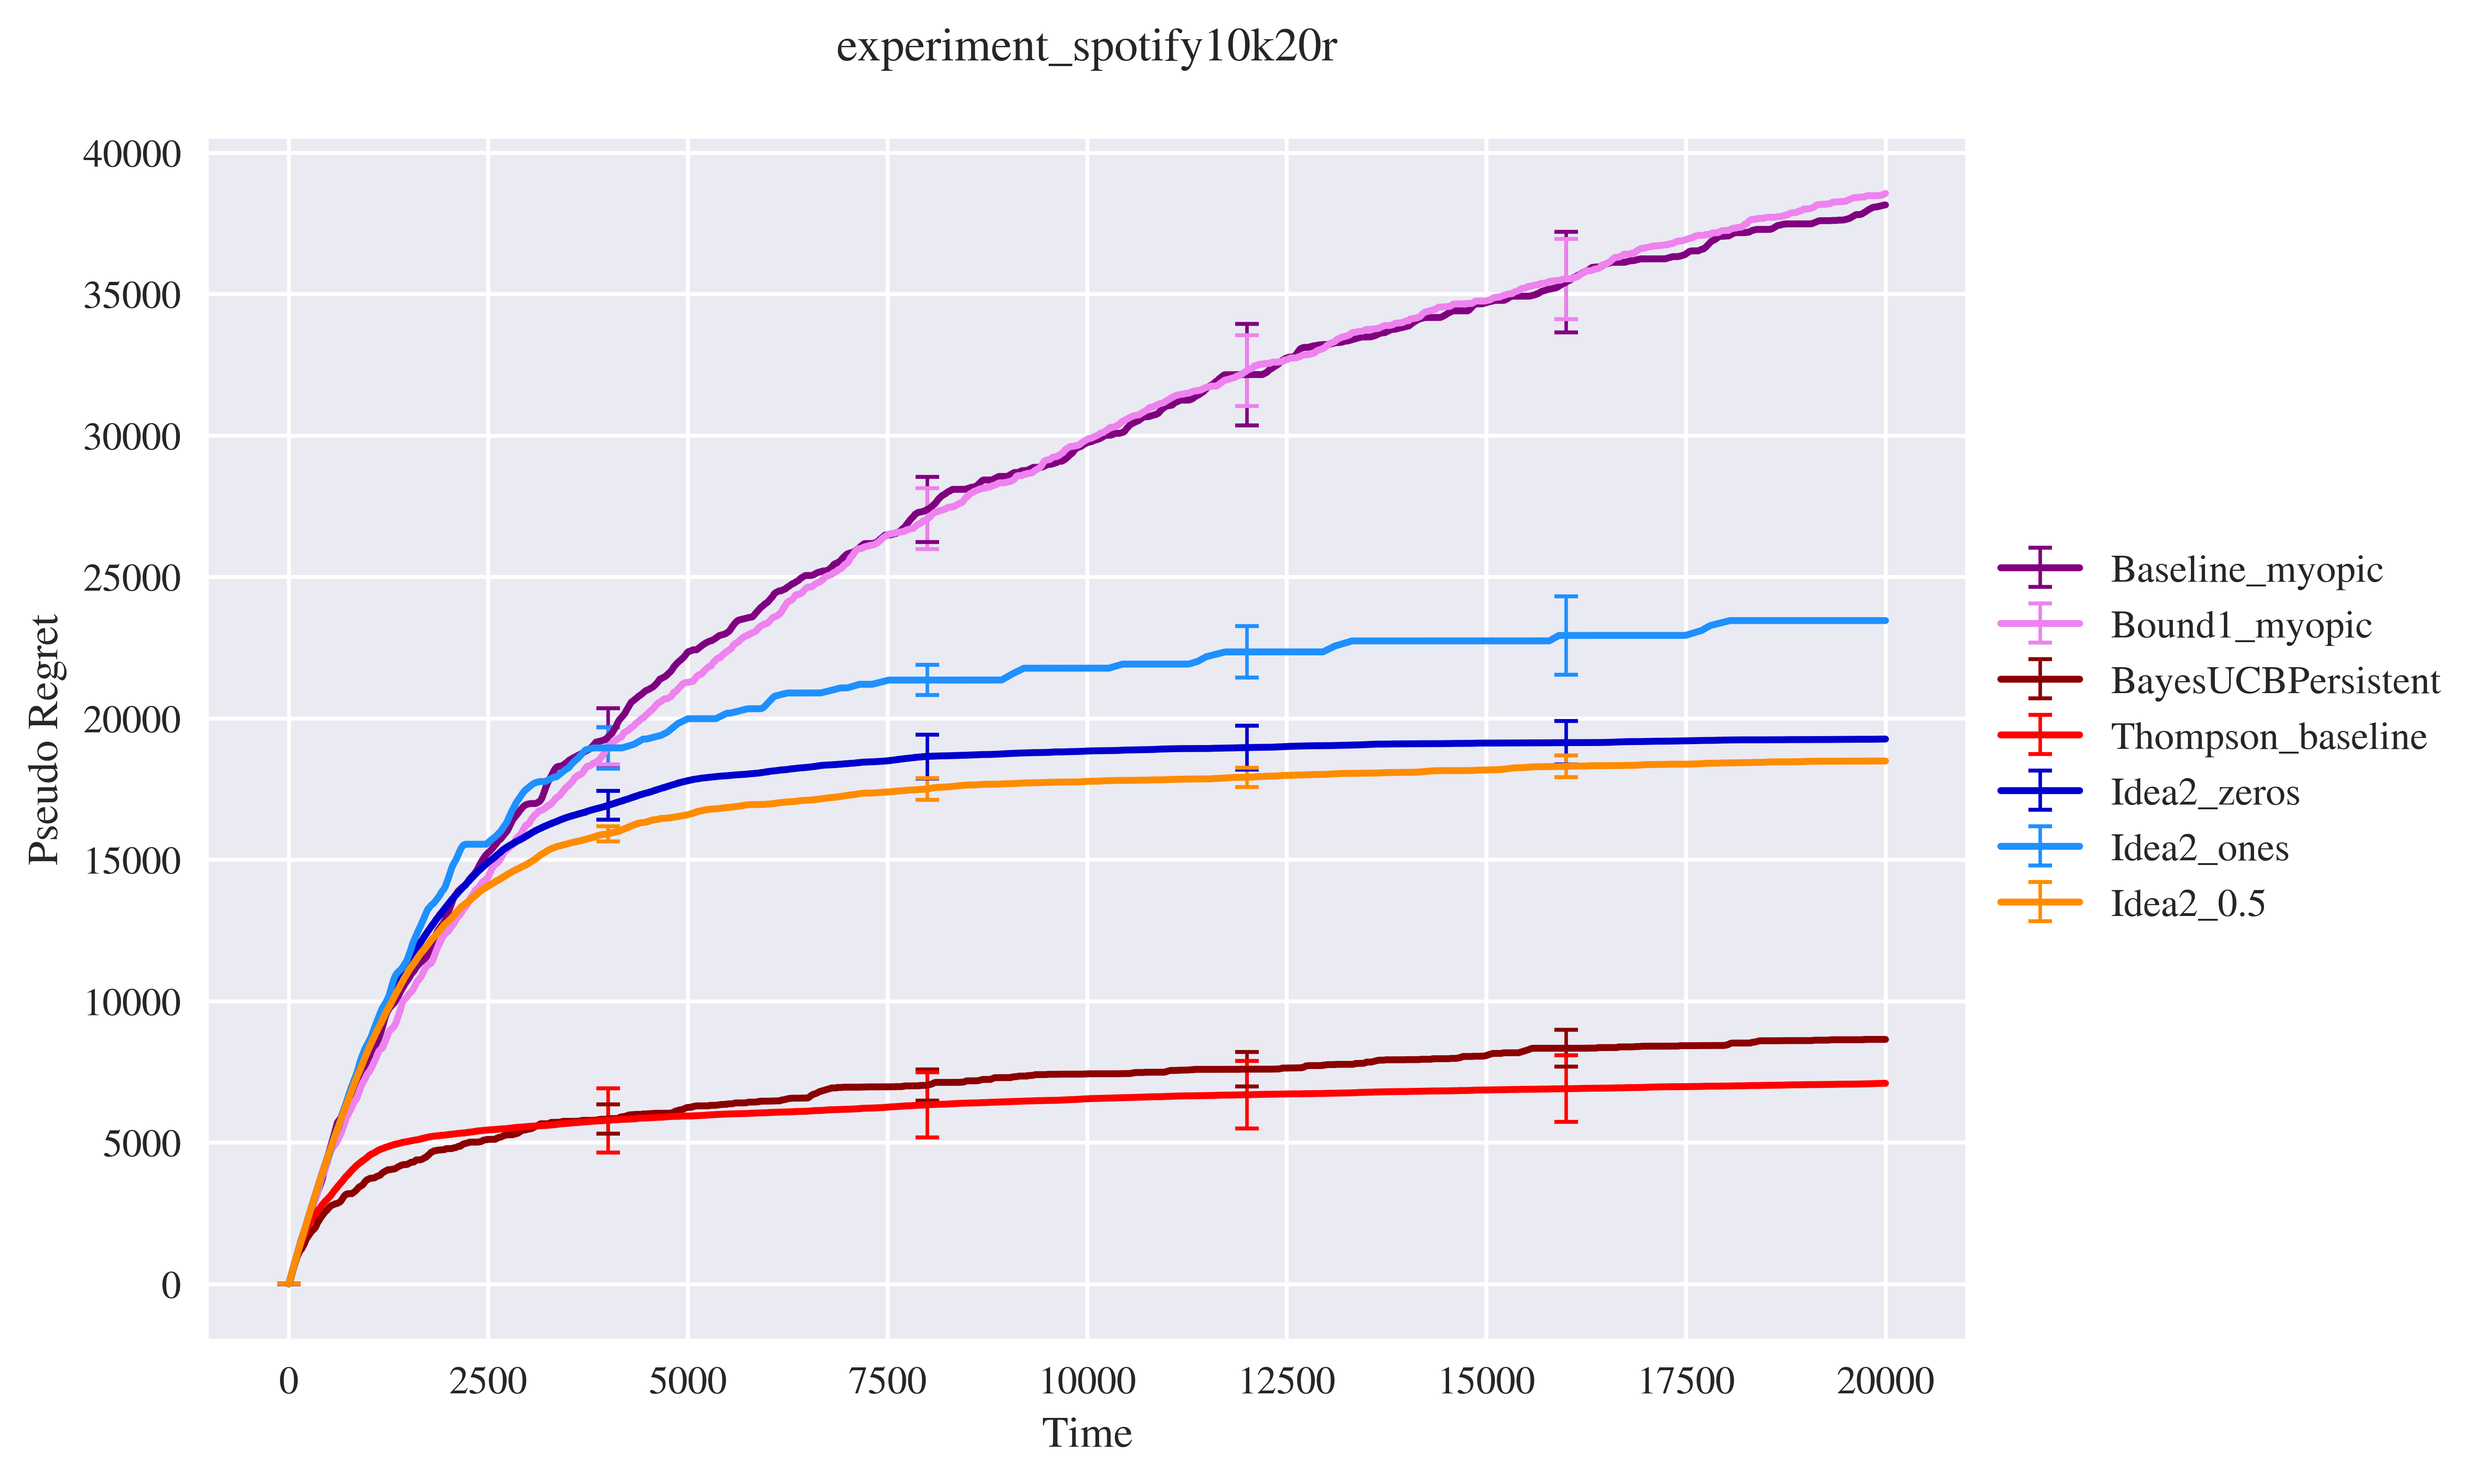
\includegraphics[width=16cm]{./images/provvisori/experiment_spotify10k20r ANALYTICS.png}
	\centering	
	\caption{PROVVISORIO Pseudo regret plot of the experiment Spotify Playlist Problem.}
\end{figure}


%RENT
\begin{figure}[H]
	\centering
	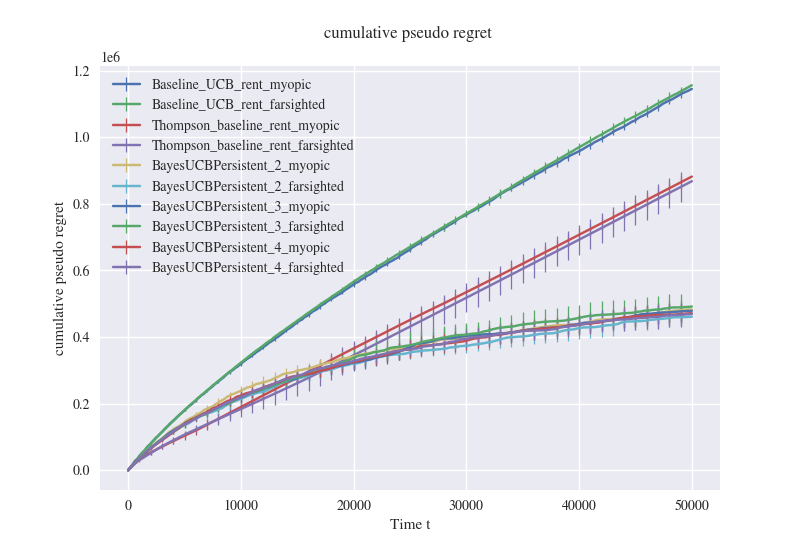
\includegraphics[width=16cm]{./images/provvisori/RENT_provvisorio.png}
		
	\caption{PROVVISORIO Normalized pseudo regret plot of the experiment Rental Pricing Problem.}
\end{figure}


\begin{figure}[H]
	\centering
	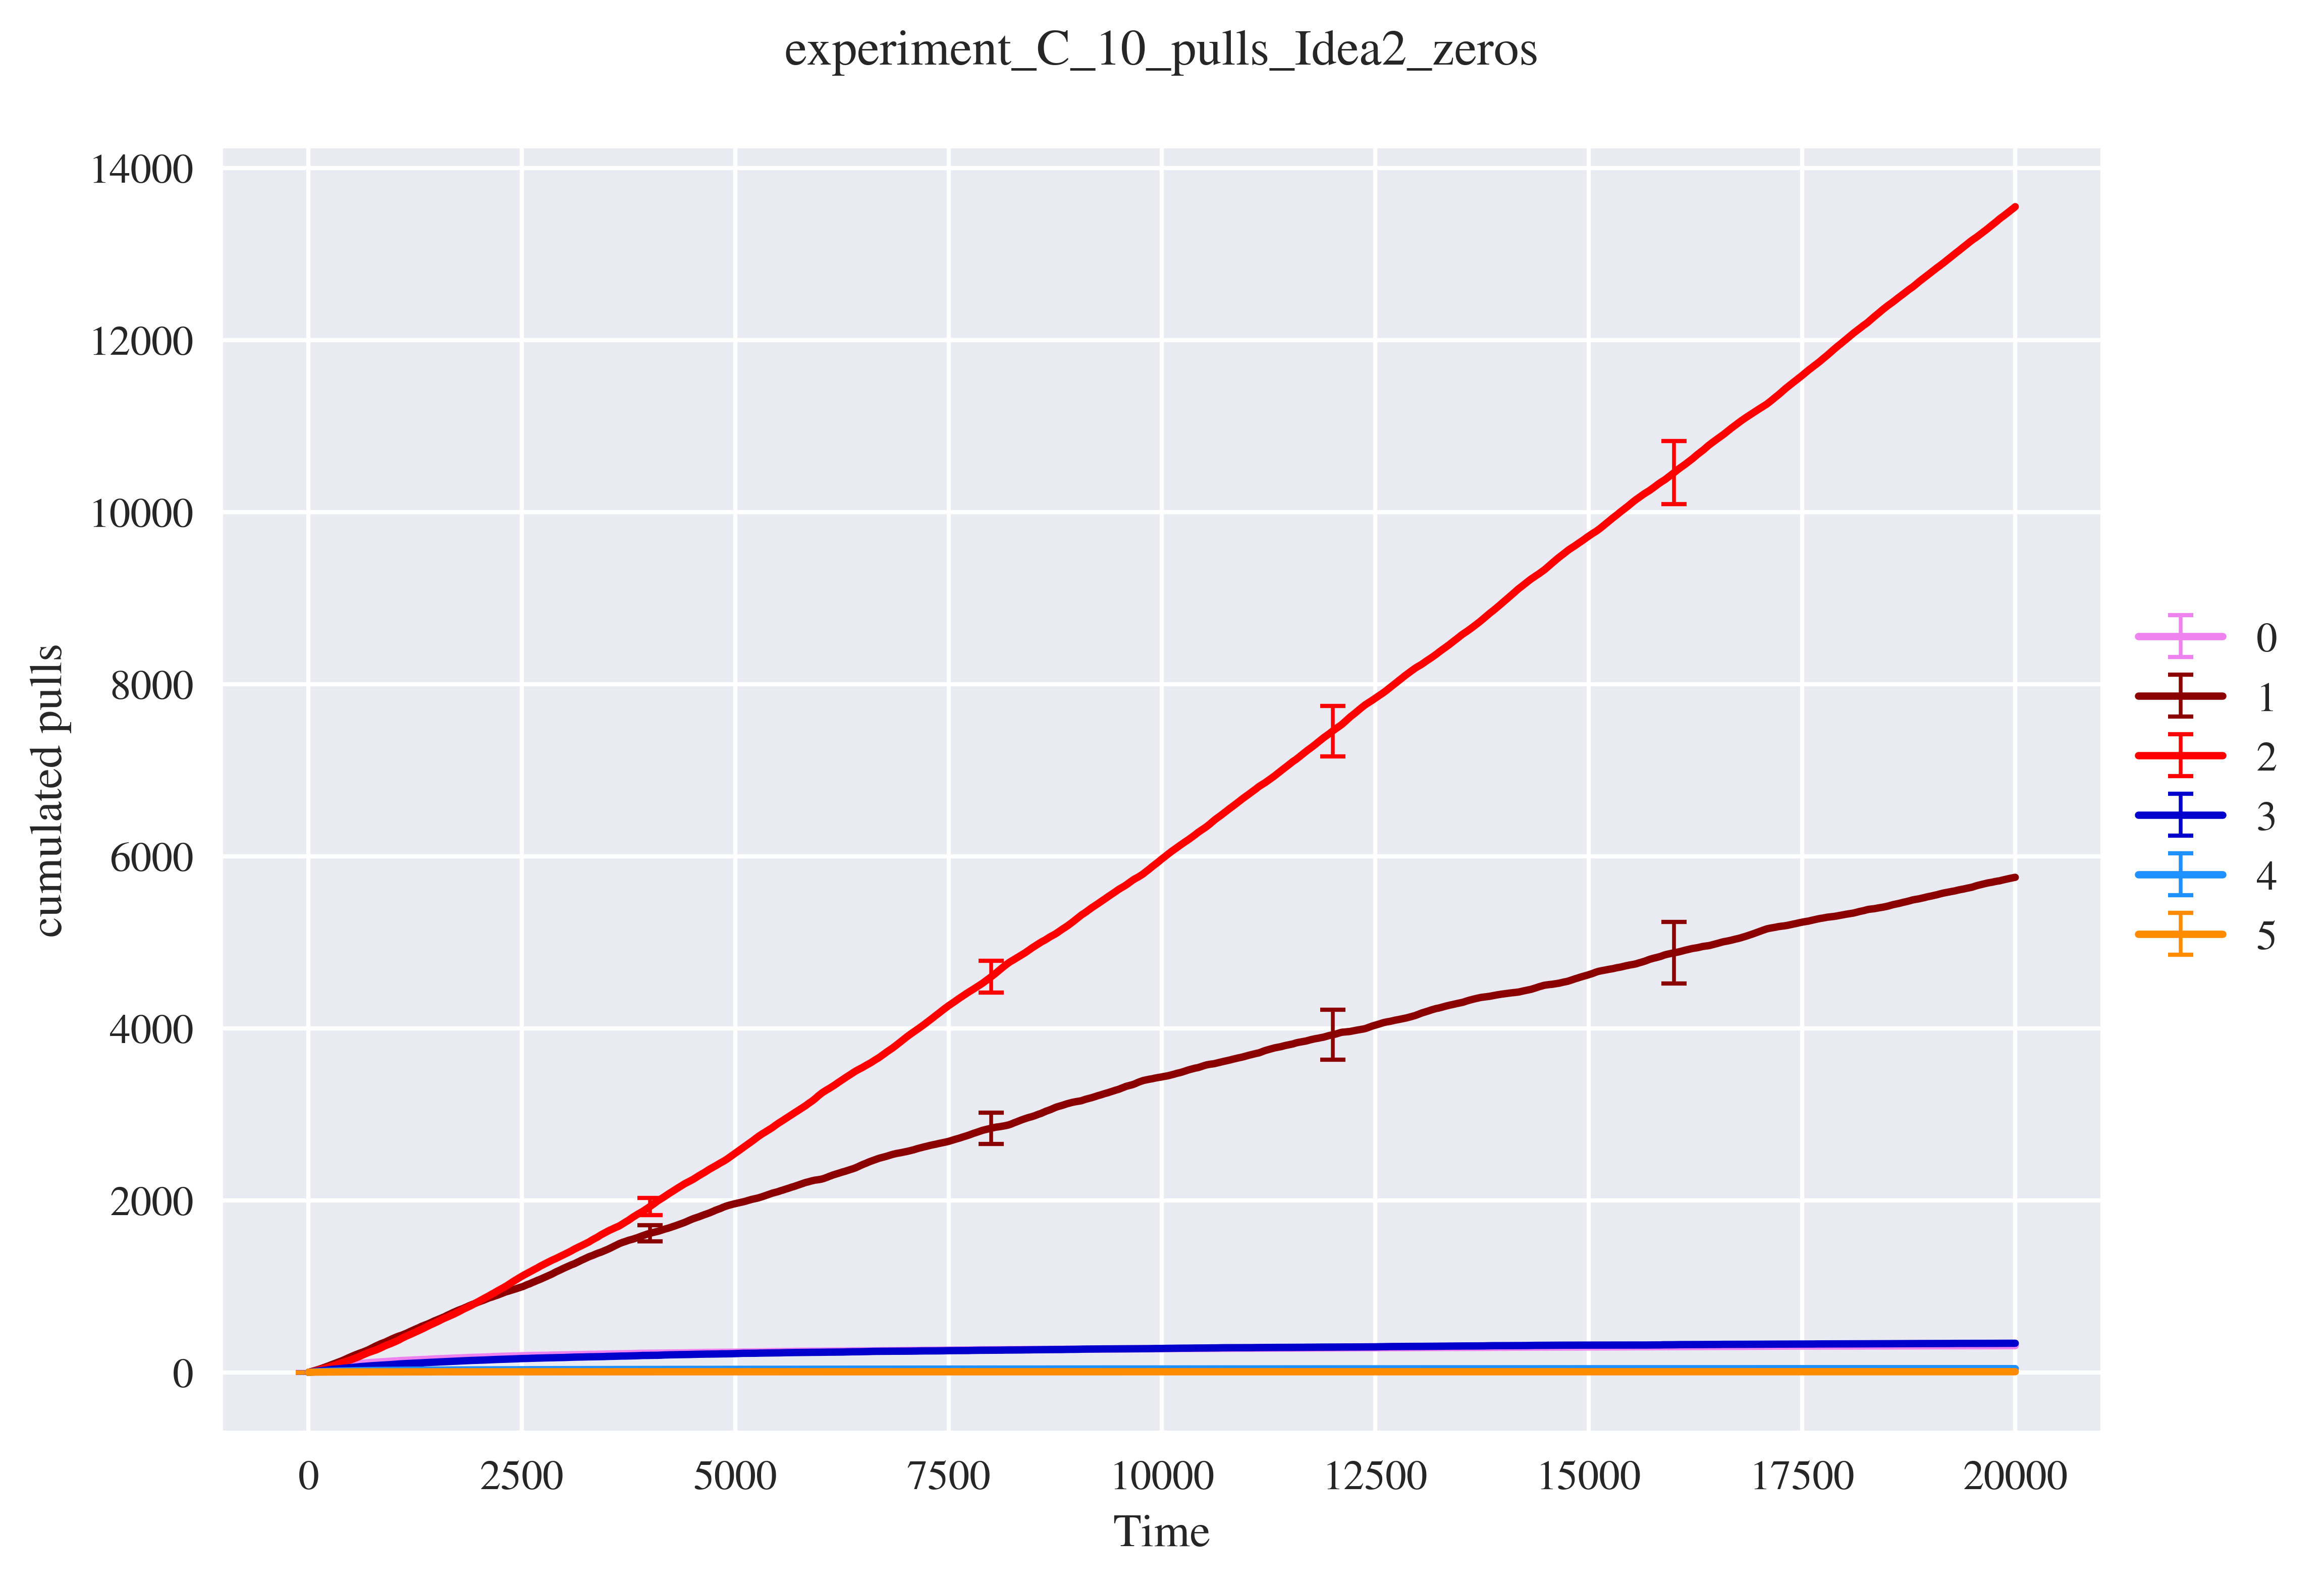
\includegraphics[width=6cm]{./images/PULLS/experiment_C_10Idea2_zeros cum_pulls.png }\quad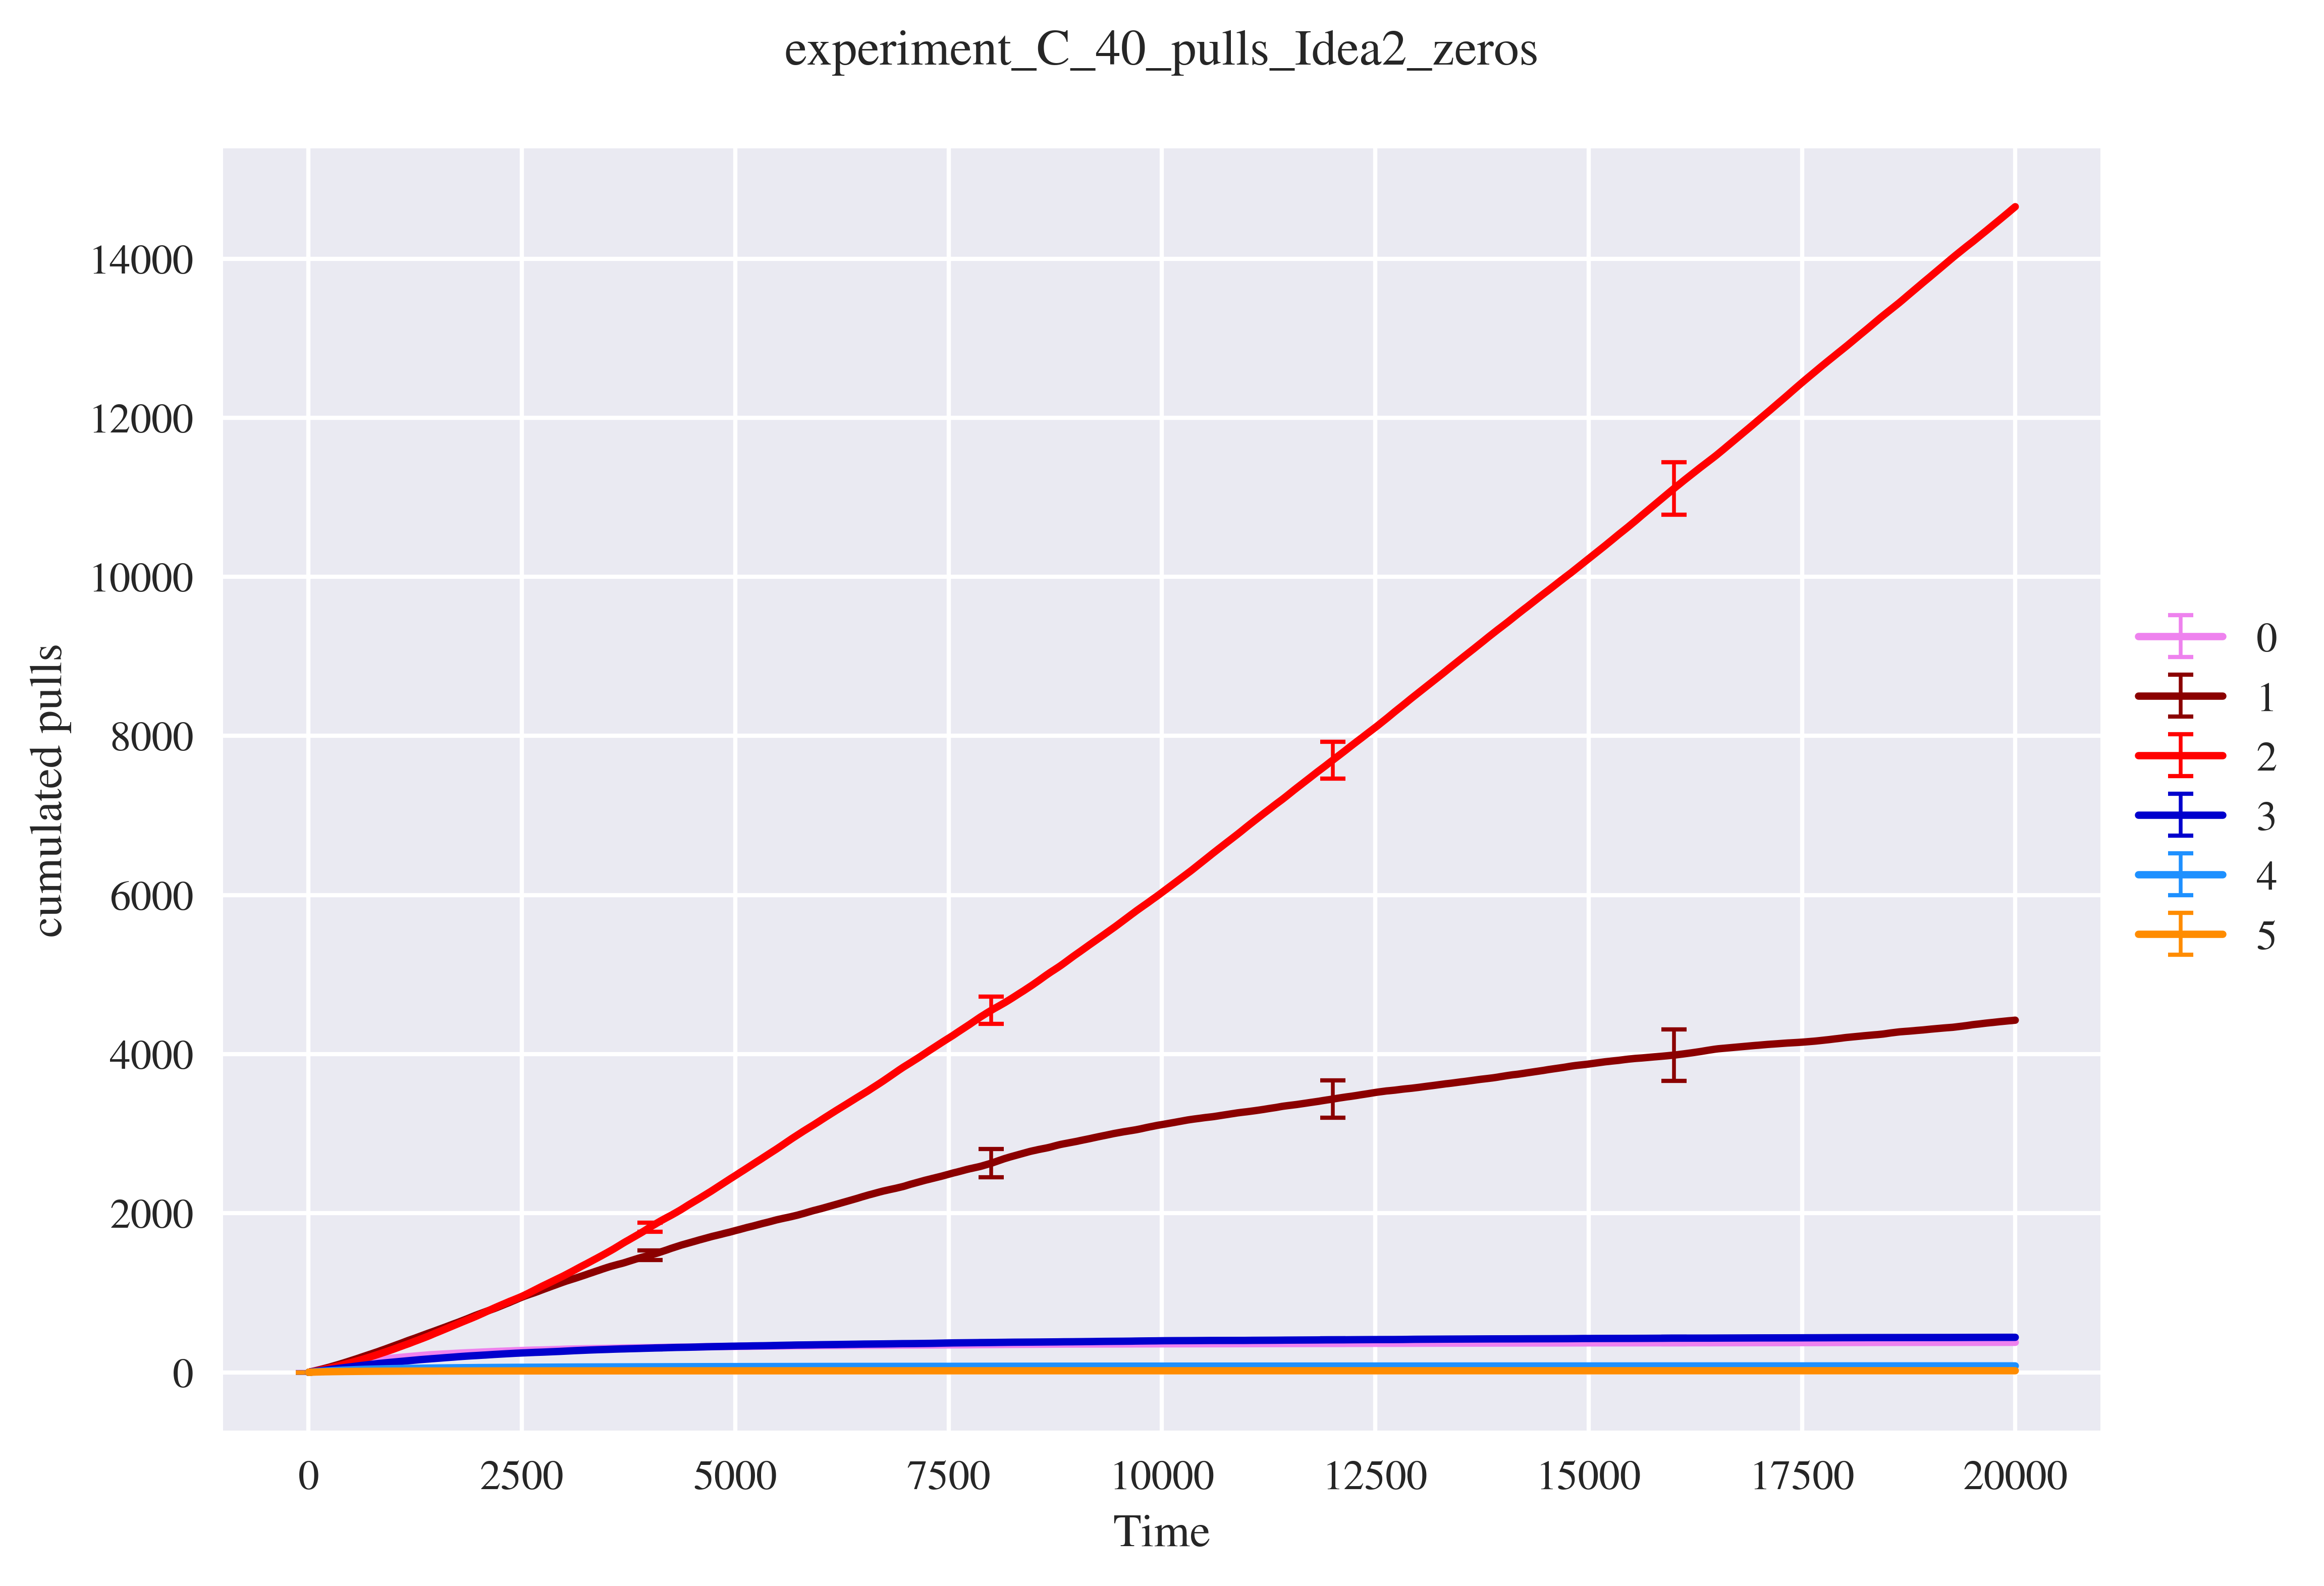
\includegraphics[width=6cm]{./images/PULLS/experiment_C_40Idea2_zeros cum_pulls.png
	} 
	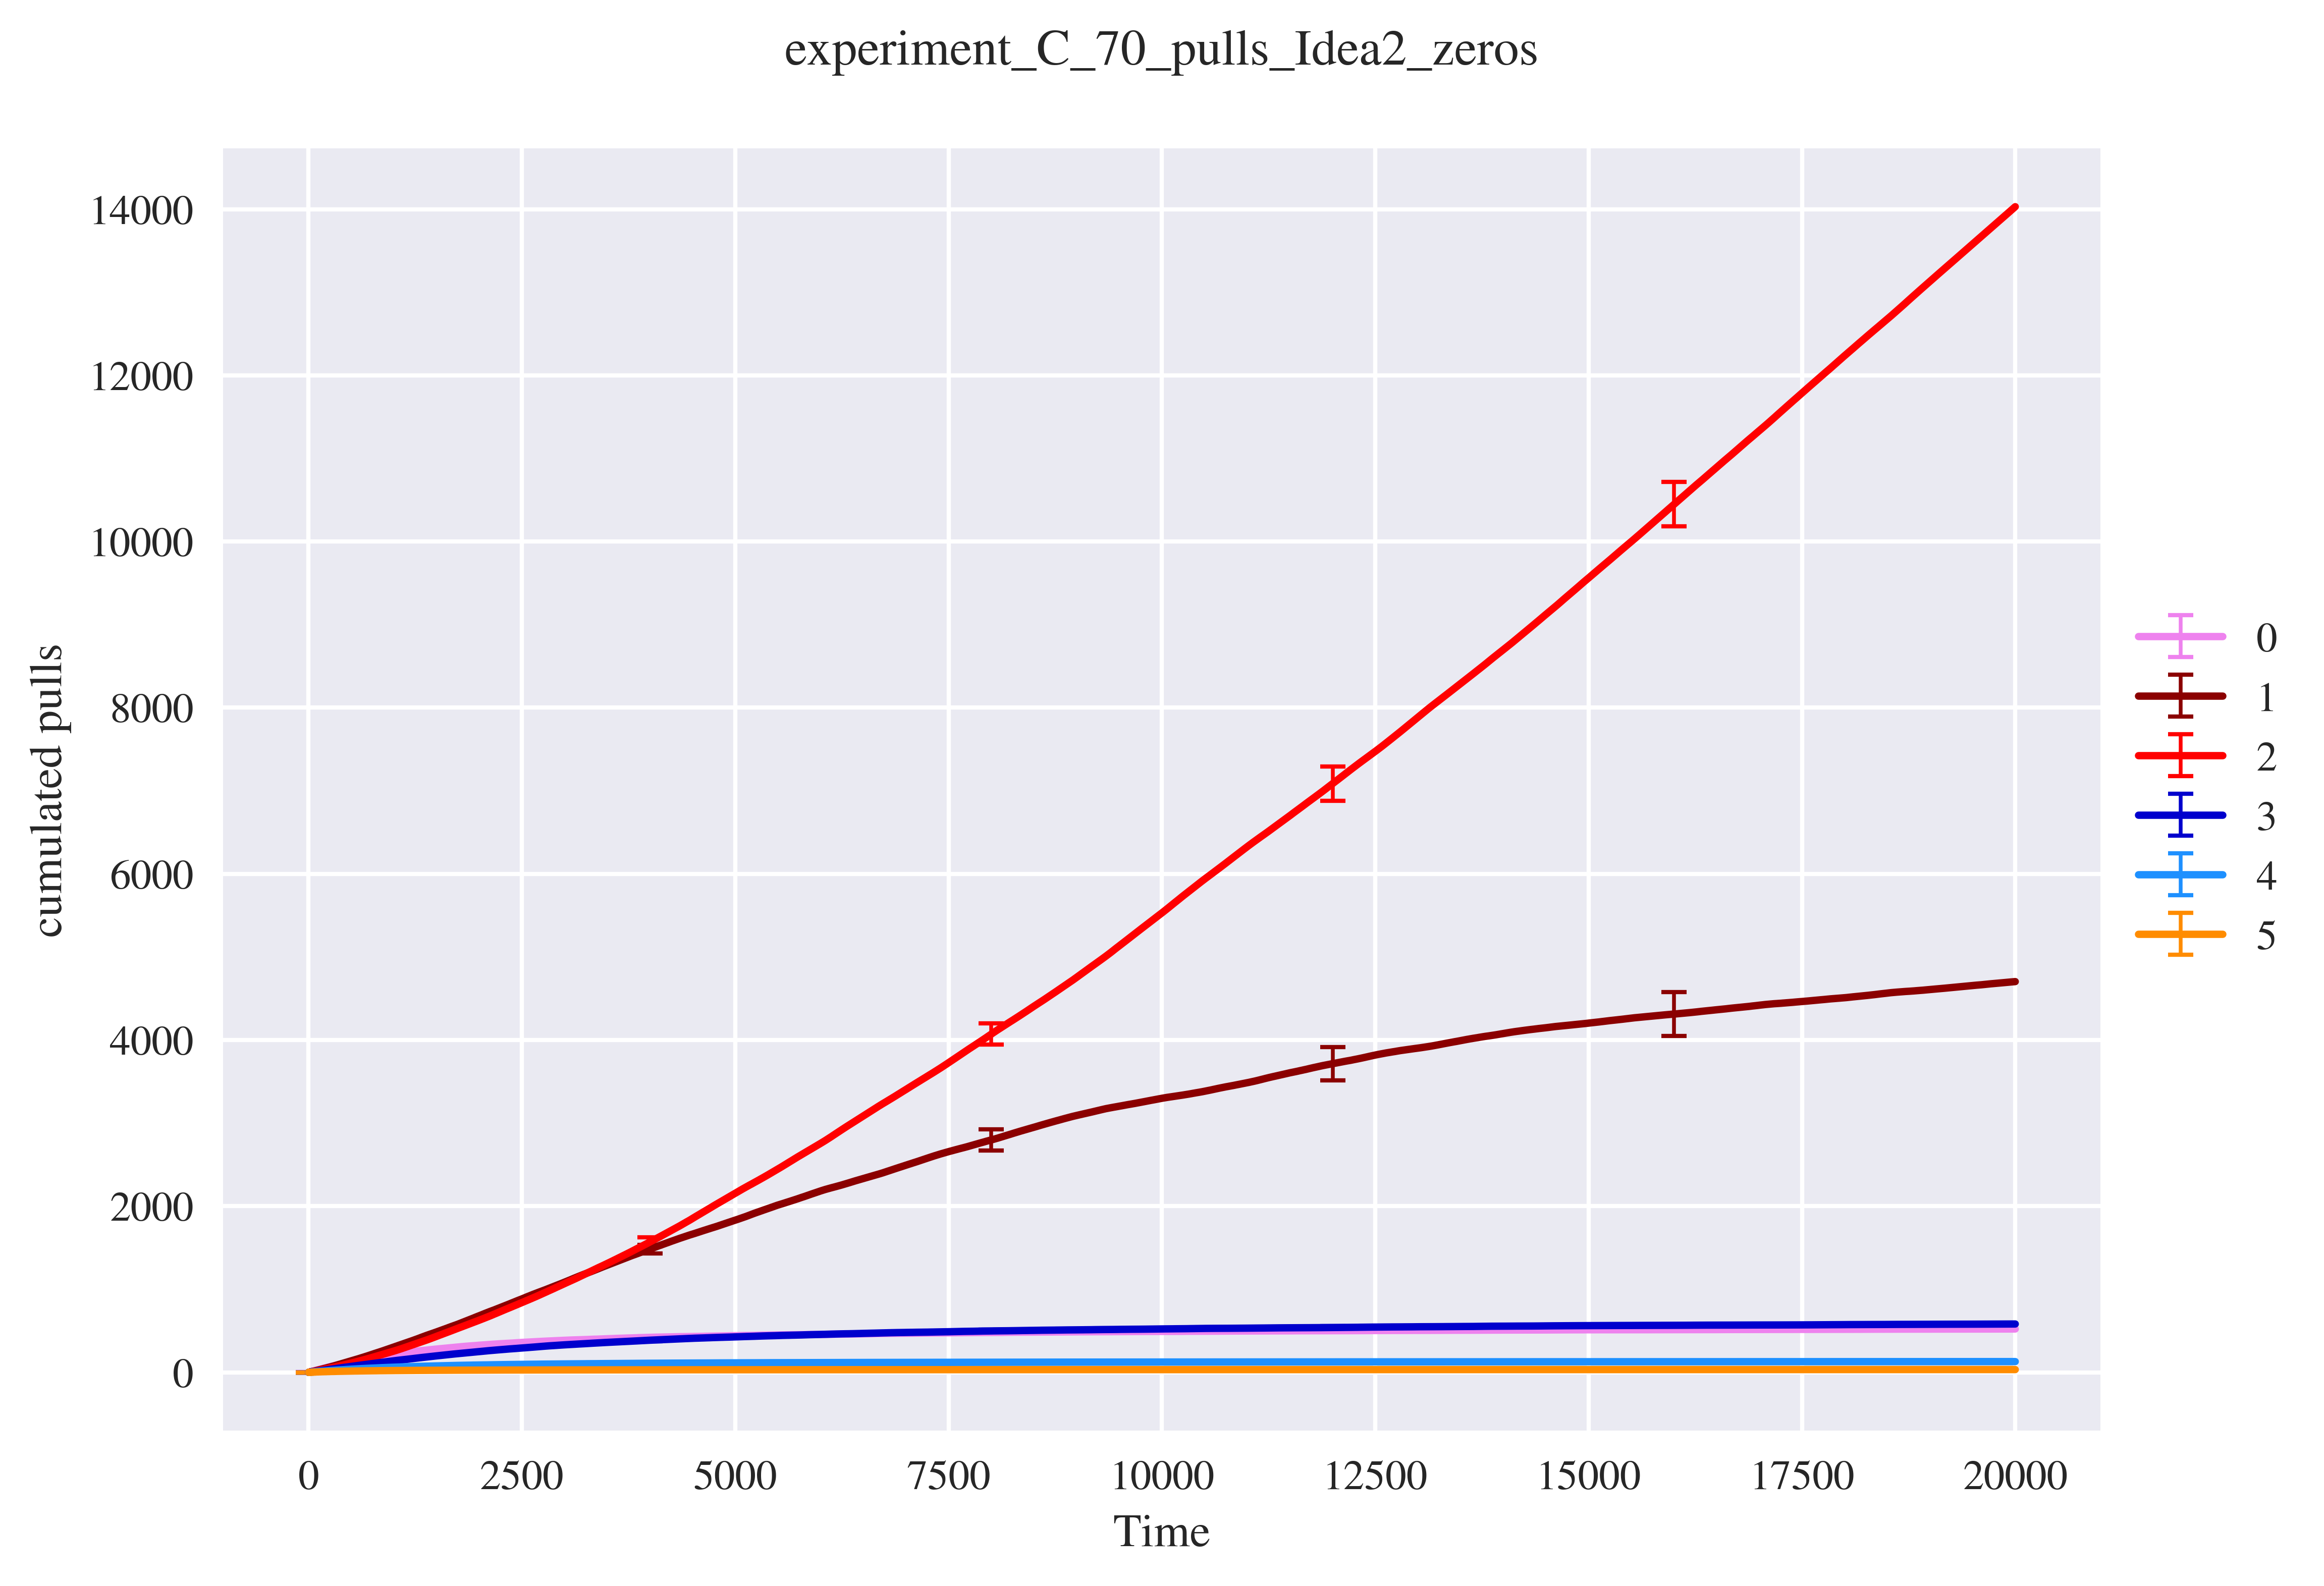
\includegraphics[width=6cm]{./images/PULLS/experiment_C_70Idea2_zeros cum_pulls.png}\quad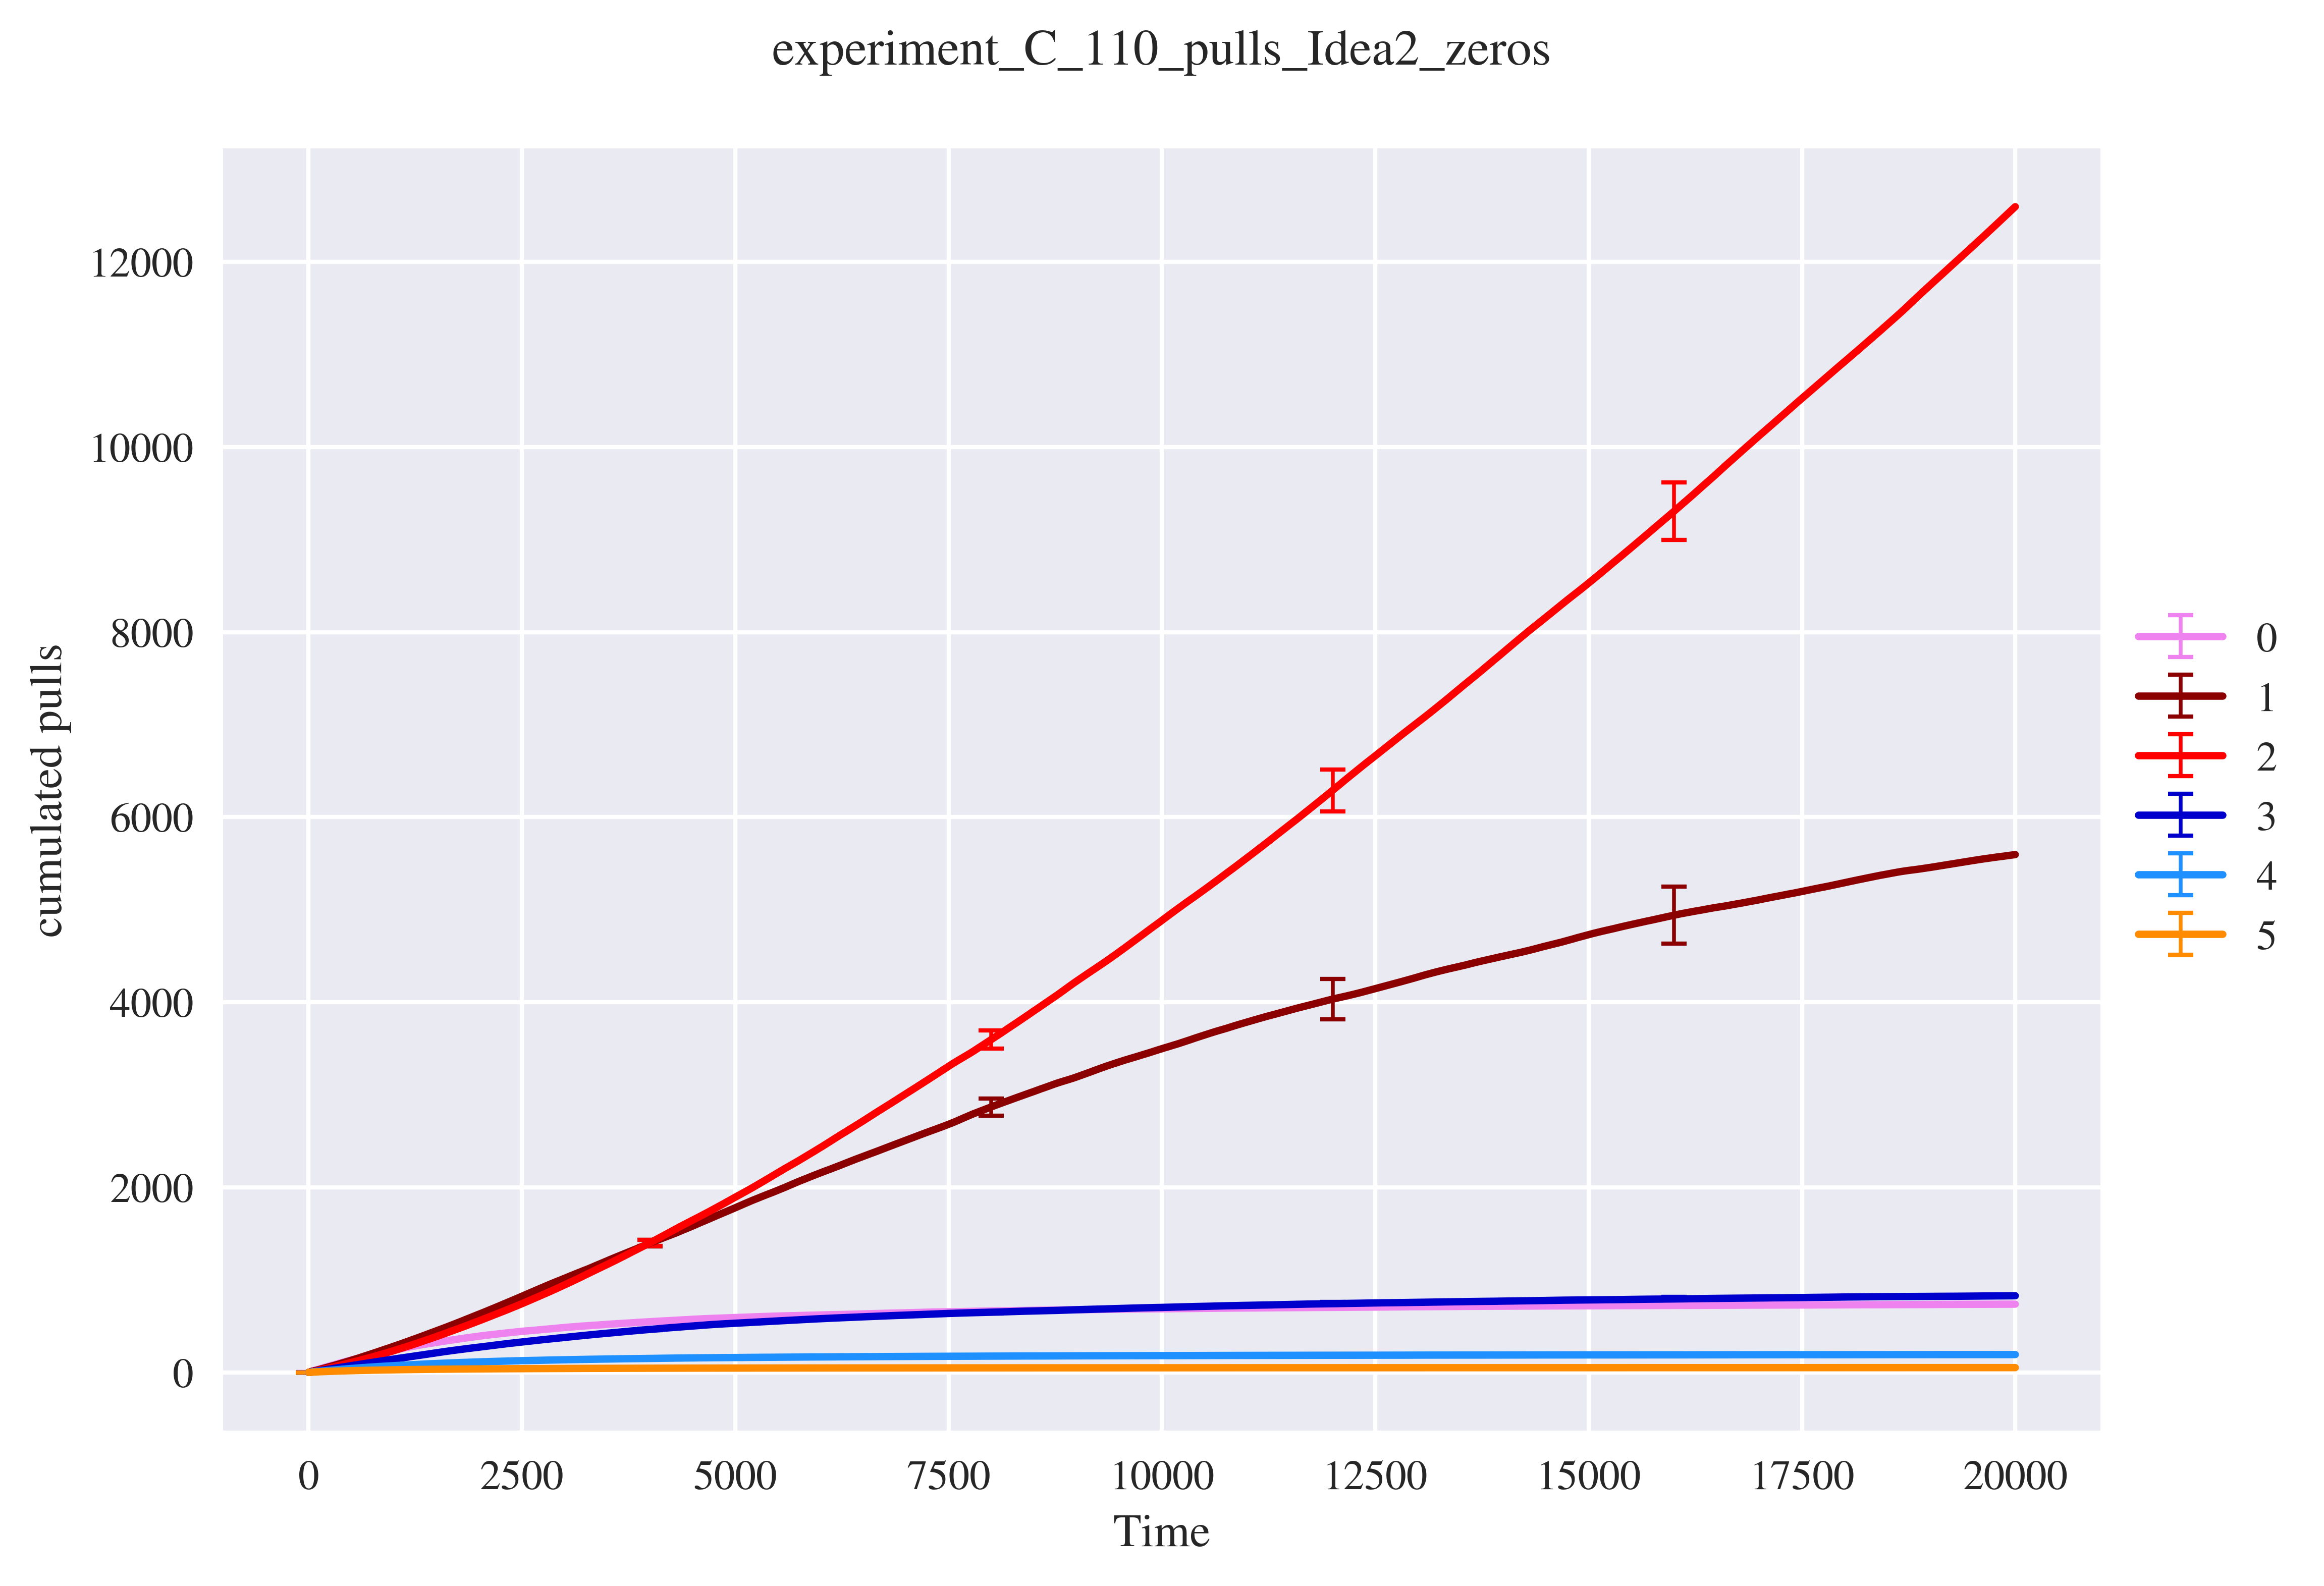
\includegraphics[width=6cm]{./images/PULLS/experiment_C_110Idea2_zeros cum_pulls.png}
	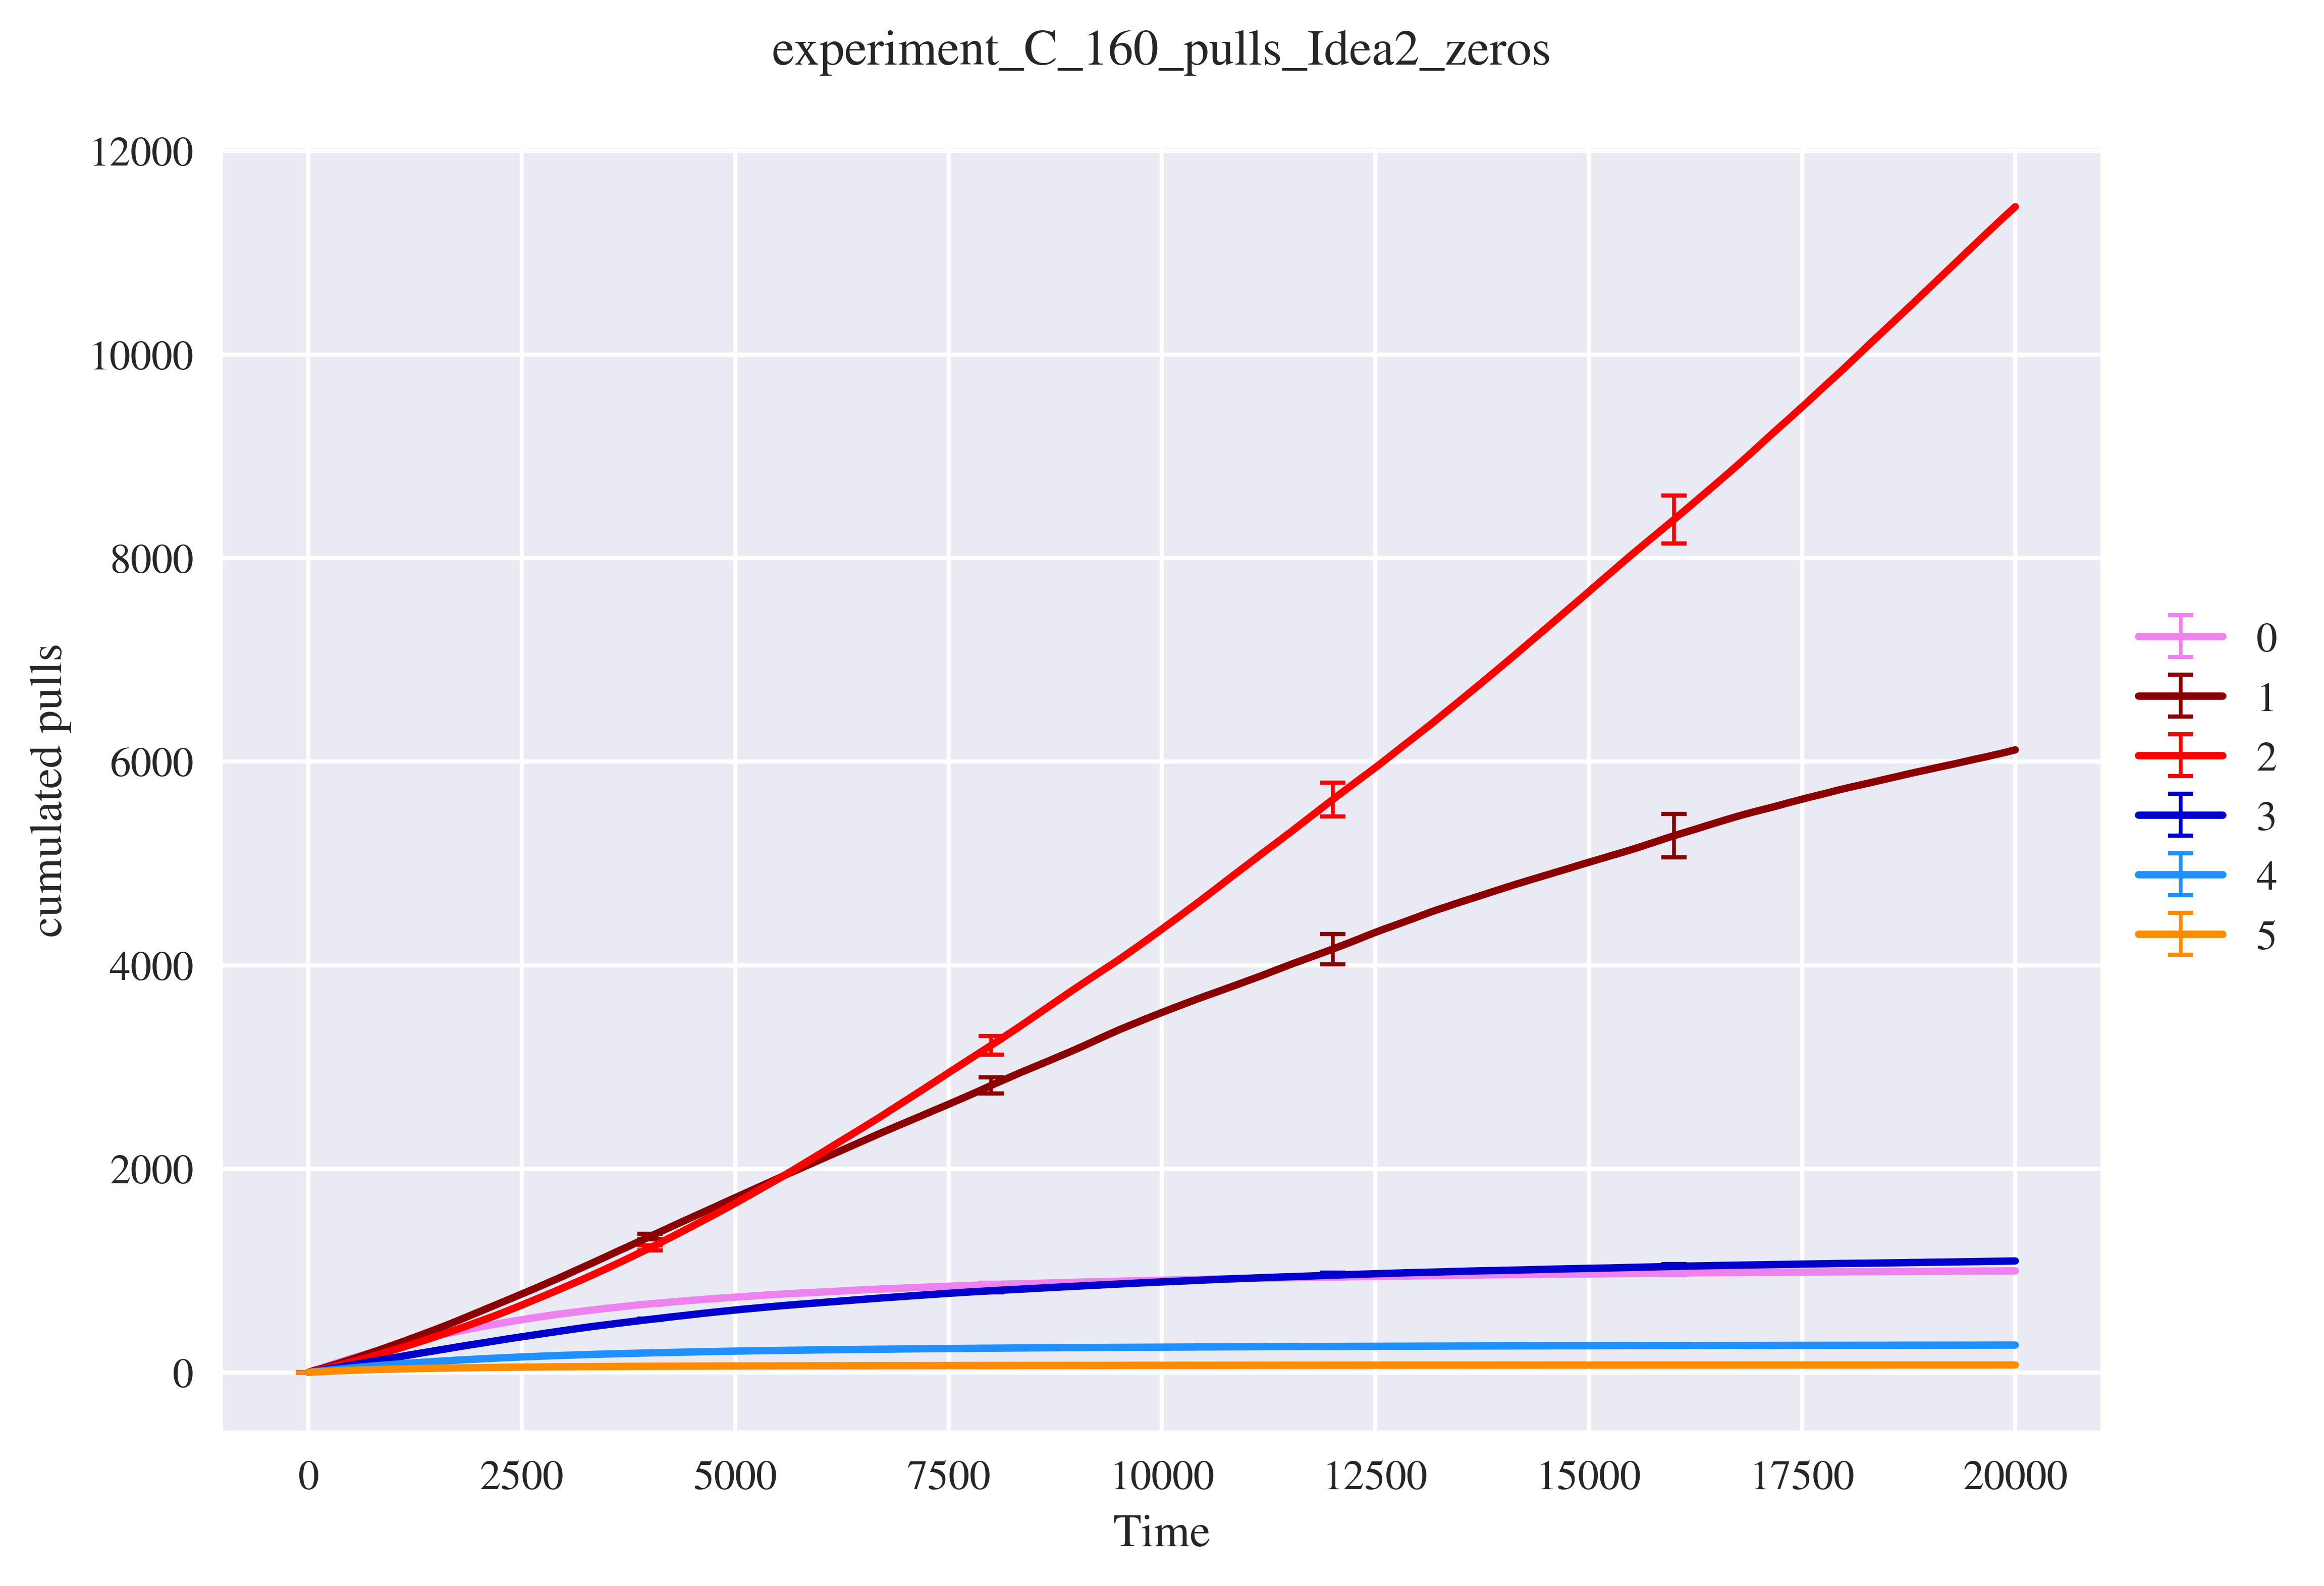
\includegraphics[width=6cm]{./images/PULLS/experiment_C_160Idea2_zeros cum_pulls.png}\quad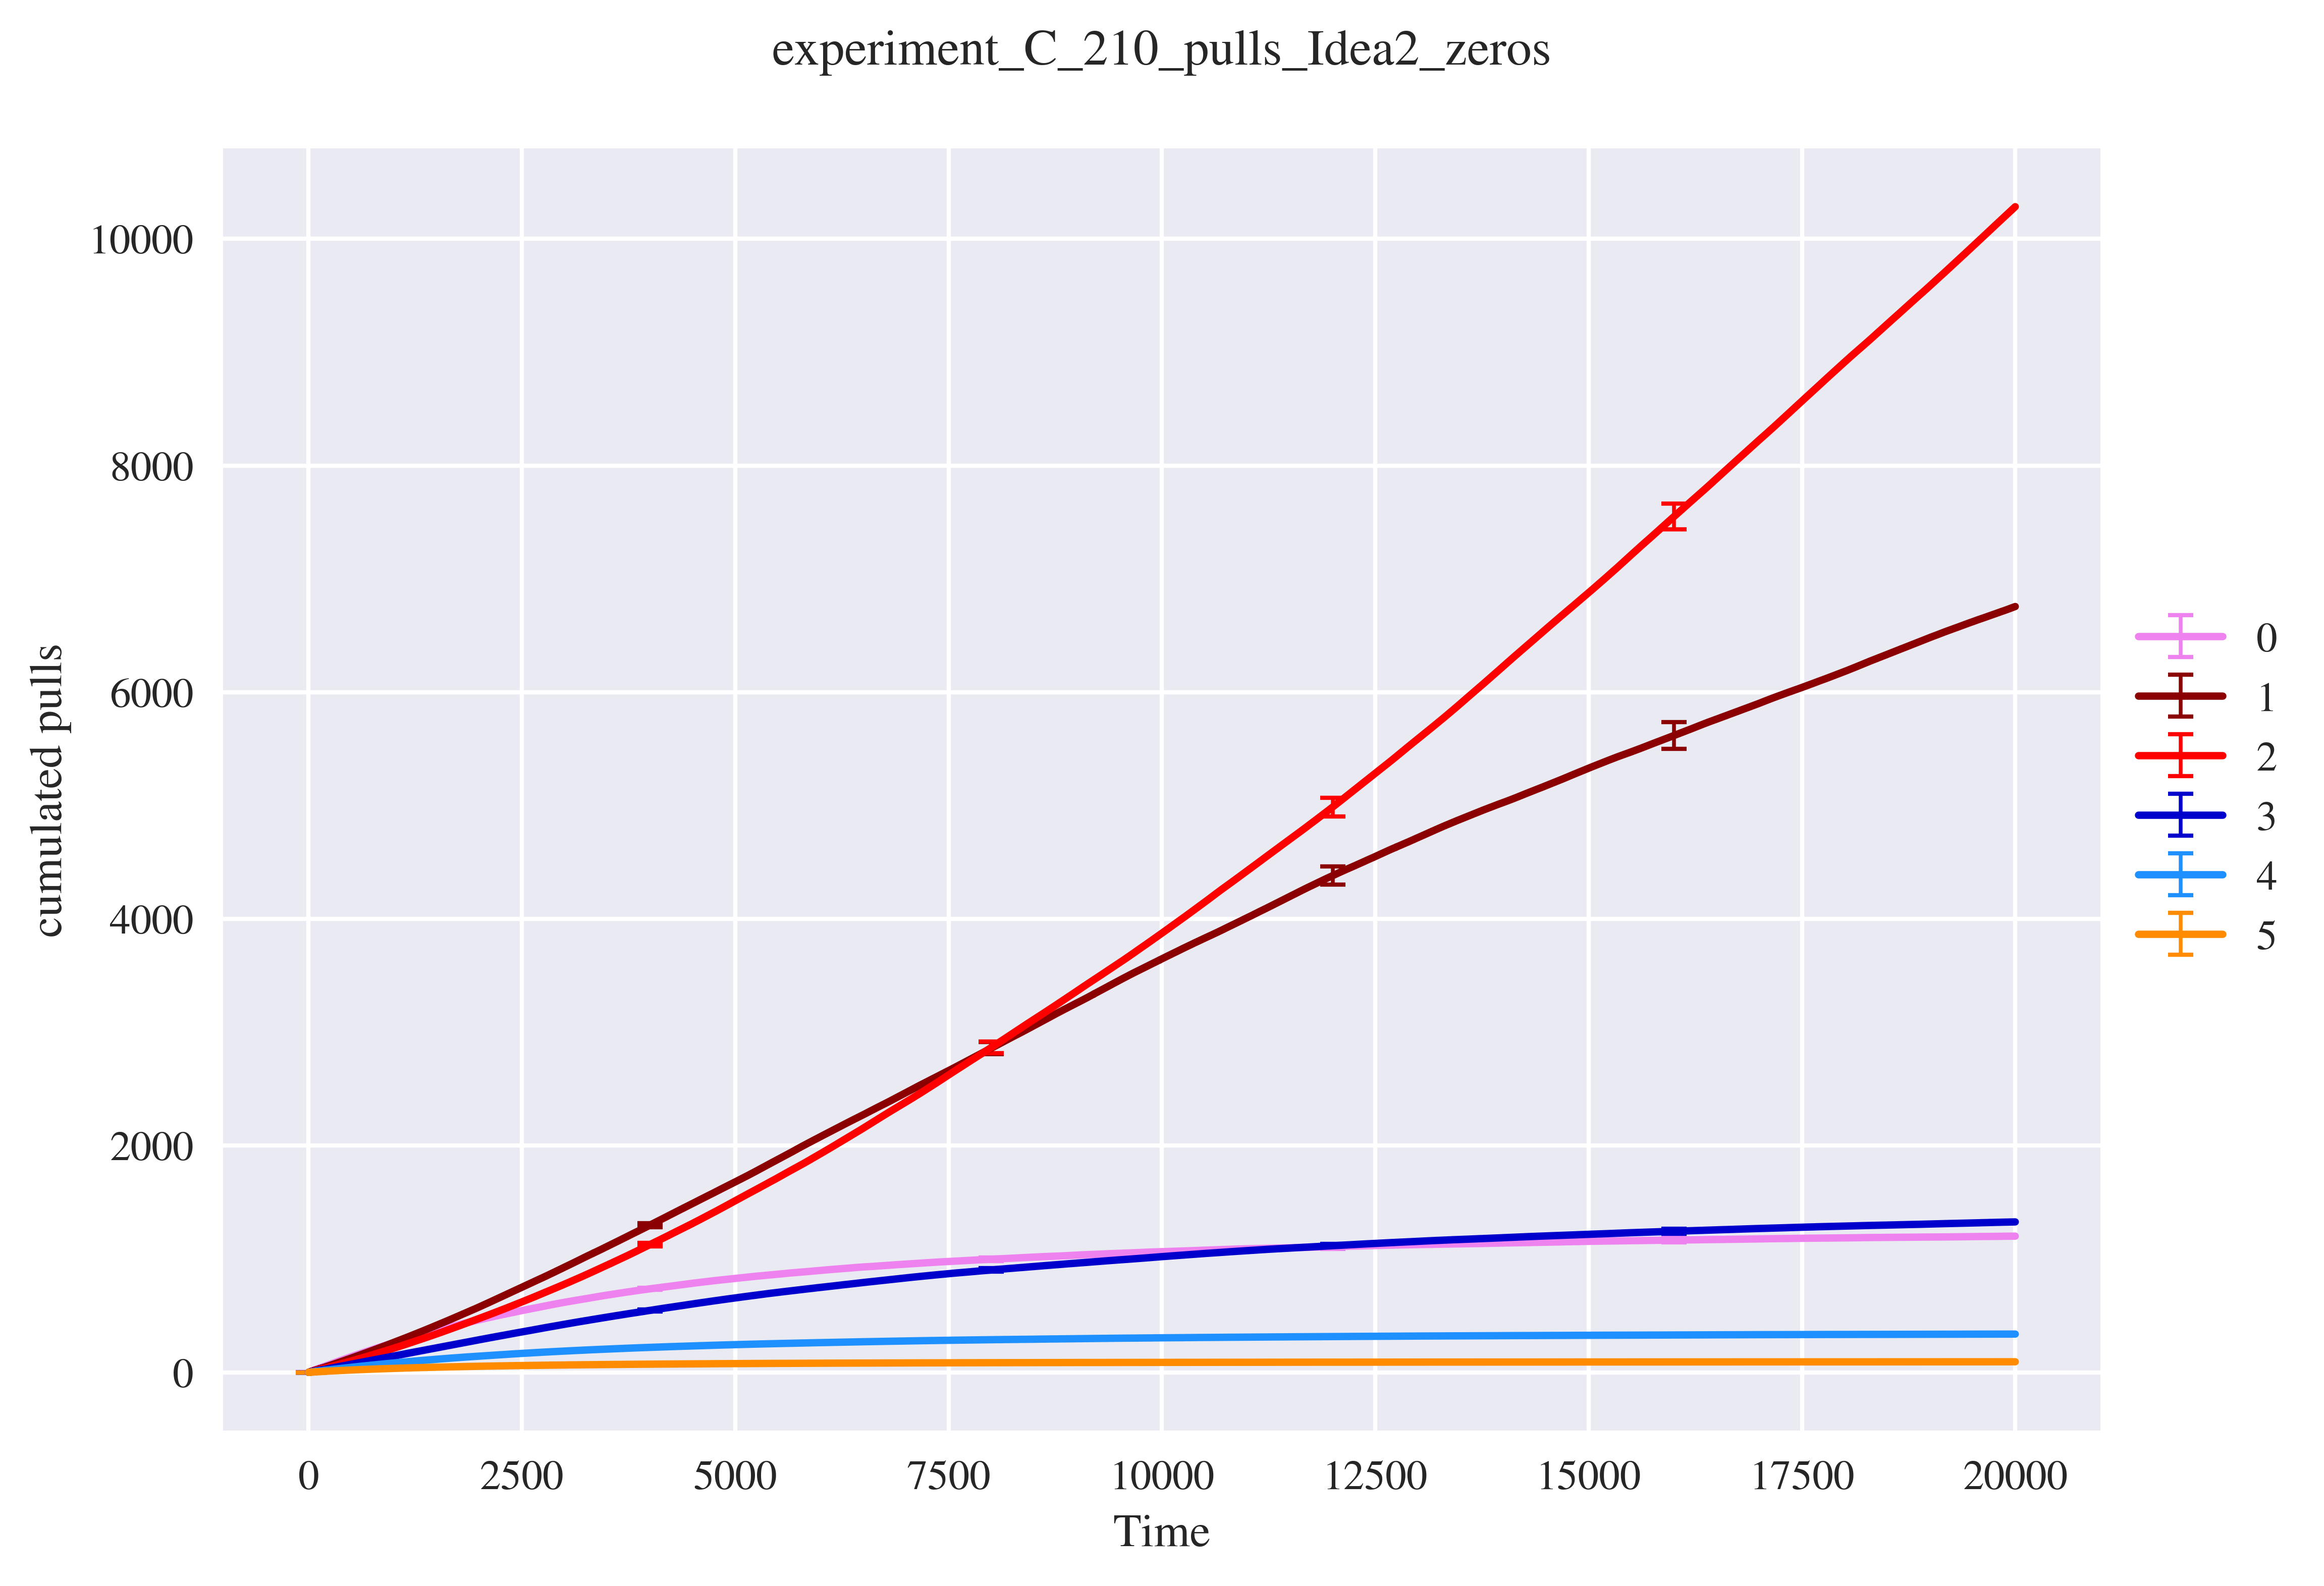
\includegraphics[width=6cm]{./images/PULLS/experiment_C_210Idea2_zeros cum_pulls.png}

	\caption{PULLS IDEA2 ZEROS C}
	
\end{figure}

\subsection{Observations}
\begin{itemize}
	
	\item in tutti gli scenari sintentici e reali, l' approccio baysiano è vincente sull'approccio frequentista.
	
	\item gli scenari sintetici sono rappresentativi di molti problemi pratici: B->Medical trial, C->Subscription.
	
	\item myopic non è mai meglio di farsighted per tutti gli algoritmi testati, in tutti gli scenari sintetici. Tuttavia solo in alcuni casi farsighted si distingue in modo evidente da myopic: Baseline in SA, Baseline in SB, Bound1 in SB, BayesUcb in C a Tmax 200. Negli scenari analizzati la configurazione non discrimina se un algoritmo è meglio di dell'altro.
	
	\item idea2 sempre peggio di idea1... capire come fare fars/myopic O idea 0.5
	
	
	\item i primi due scenari sintetici ( A e B) pur avendo una diversa concenzione, presentano lo stesso ranking disegnando una situazione molto simile. BayesUcb vince su tutti. A seguire TS -I2 - B1-Baseline.
	
	\item mentre bound1 e baseline hanno un andamento simile nel piegare, idea 2 ha una forte esplorazione nella fase iniziale per poi piegare bruscamente. (piegare= imparare arm migliore) . Potrebbe essere la costante che moltiplica $\ln t$ nel bound?
	
	\item lo scenario c evidenzia una situazione interessante, ci fa vedere come idea 2 soffra maggiormente l'aumento di tmax a parità di scenario. bound1 in questo scenario è quasi indistinguibile alla baseline.
	
	\subsubsection{spotify}
	
	\item bound1 e baseline non sono distinguibili -> ragionevole, siamo in general peristency e il reward è distribuito con stessa probabilità dall'inizio alla fine il vantaggio di anticipare è ridotto (non c'è).
	\item anche sui bayesiani si riflette in quanto TS si scambia con ByesUCB
	
	\item in generale gli algoritmi imparano e dopo 2500 iterazione TS smette di crescere, ovvero riesce a consigliare quasi sempre la playlist migliore. Promettente per implementazioni più approfondite.
	
	\subsubsection{rent}
	\item il problema appare molto più difficile, in quanto ne la baseline ne TS riescono ad imparare nell'orizzonte prefissato. BayesUCB performa molto meglio superando entrambi.
	
	\item nel caso degli affitti risulta inappropriato l'utilizzo di mab persistent con questi valori. la simulazione affitta ad ogni mese una nuova casa, e dopo 50000 mesi il prezzo ottimo ""non è stato ancora trovato"". Tuttavia semplificando il problema alterando i dati...
	
	
	
		
	
\end{itemize}

\chapter{Conclusions}\label{C6}
The Multi-Armed Bandit model is an important framework for decision making under uncertainty, as it presents one of the clearest examples of the trade-off between exploration and exploitation. In problems of this type, an agent, at each time instant, is required to choose an action among a given set of actions. Each action, when chosen, generates a reward for the agent. The goal of the agent is to maximize the cumulative reward over a finite time horizon. Although the standard bandit model assumes that the reward is a real number immediately available after an action has been taken, this assumption is inappropriate for a variety of scenarios. In this thesis, motivated by real-world application needs, we studied the specific case in which the reward deriving from an action is spread over the time following the taking of the action, naming this setting persistent reward. Applications that fall under persistent reward include, for example, dynamic pricing, web content optimization, recommender systems and adaptive clinical trials.

We firstly formalized a new bandit model, namely Multi-Armed Bandit with Persistent Reward (MAB-PR), suitable to handle persistent reward scenarios. Then, we designed a wide family of algorithms, which includes both Bayesian and Frequentist algorithms, tailored to tackle this bandit model. Our major interest was to develop and analyze novel algorithms able to exploit the partial information obtained during the reward acquistion process. At this purpose, we introduced two different approaches: the bin-wise approach and the non-terminated approach. The former takes advantage of the fact that the total reward deriving from an action can be seen as a sum of smaller rewards (bins) acquired at each time instants after the take of the action. On the other hand, the latter, exploits the not yet terminated reward acquisition processes considering them terminated by faking the part of the process not yet occurred with fictitious information. The algorithms that base their operating criteria behind these approaches have been compared with those that evaluate the reward as a unique variable available only at the end of the acquisition process that, for this reason, we considered as baselines. The baselines algorithms, which do not exploit partial information, come from the Delayed MAB literature. Indeed, to consider the reward as a number available after that the acquisition process is terminated, reduces the persistent reward problem to a delayed reward problem.

For the Frequentist algorithms we provided theoretical guarantees which, under certain conditions, state that both the baseline and the bin-wise algorithm PR-BW-UCB-P achieve a regret bound of the order of $O(\Tmax^2\ln t)$. Furthermore, we proved that the algorithm PR-NT-UCB-P, which relies on the non-terminated approach, achieves a regret bound of the order of $O(\Tmax\ln t)$.

We performed a thorough experimental analysis of the developed algorithms which includes both synthetic-data settings and real-data settings. The experimental results show that, in the large majority of the settings analyzed, the novel algorithms that exploit partial information achieved better results compared to the baselines pertaining to the same group (Bayesian and Frequentist). This is satisfactory since the baseline algorithms represent the state-of-the-art to tackle the addressed problems. Furthermore, the theoretical results are perfectly reflected in the outcome of the experimental analysis, where, for each addressed scenario, the algorithm PR-NT-UCB-P outperforms all the other Frequentist algorithms when a sufficient time horizon is provided. Experimental evidence shows that the way the reward is distributed over the time severely affects the performance of the algorithms. This is actually not surprising. Indeed, it is reasonable to think that if a large portion of the total reward generated by an action is concentrated immediately after that the action has taken place, the advantage of capturing this information without waiting is remarkable. On the contrary, if the reward is uniformly distributed over the timespan following the take of an action, the advantage gathered from an early evaluation is limited. In the worst case, it can even be misleading to exploit partial information if, in an initial phase, these are not representative of the total reward deriving from the take of an action. In our analysis, the Bayesian algorithms always achieve better performance compared to the Frequentist ones. We show experimentally that the Bayesian way to manage the exploration exploitation trade-off is the best in the persistent reward scenario. This confirms what we expected since previous works shows that Thompson Sampling, which inspired our Bayesian algorithms, is more robust under delayed feedback thanks to its randomness \citep{Chapelle2011Thompson}.


The main future directive of this work is to prove theoretical bounds for all the algorithms which have not been sufficiently theoretically analyzed, in particular the ones pertaining to the Bayesian family. Our experimental results emphasised how the persistent reward settings is sensible to the the way in which the reward is distributed along its acquisition process. An interesting research line could be to theoretically formalize this aspect and to devise new strategies which consider it. Alternatively, could be also interesting to prove criteria that, based on the reward distribution along its acquisition process, determine when it is convenient to approach a specific persistent reward scenario with an algorithm that exploits partial information. Other possible extensions can be achieved by combining other MAB variants with the MAB-PR model. In particular, we believe that the two most limiting assumption are: (i) the absence of side information; and (ii) the stationarity of the reward. Indeed, these two assumptions are very significant in a lot of real problems that could be modelled as MAB-PR problem. For example, in a recommendation task, the absence of side information means that the algorithm considers that all the users to be served are identical, or, in a dynamic pricing problem, the stationarity of the reward implies that the algorithm is not able to react to the market variations. Indeed, could be interesting to mix our MAB-PR model with Contextual Bandits \citep{contextual} or Seasonal Bandits \citep{di2020linear} to cope with (i) and (ii) respectively.





\bibliographystyle{abbrvnat}
%\bibliographystyle{apacite}
\bibliography{bibliografia}

\end{document}